%%%%%%%%%%%%%%%%%%%%%%%%%%%%%%%%%%%%%%%%%%%%%%%%%%%%%%%%%%%%%%%%%%%%%%
%%  disstemplate.tex, to be compiled with latex.                     %
%%  08 April 112002     Version 4                                    %
%%%%%%%%%%%%%%%%%%%%%%%%%%%%%%%%%%%%%%%%%%%%%%%%%%%%%%%%%%%%%%%%%%%%%%
%%                                                                   %
%%  Writing a Doctoral Dissertation with LaTeX at                    %
%%      the University of Texas at Austin                            %
%%                                                                   %
%%  (Modify this ``template'' for your own dissertation.)            %
%%                                                                   %
%%%%%%%%%%%%%%%%%%%%%%%%%%%%%%%%%%%%%%%%%%%%%%%%%%%%%%%%%%%%%%%%%%%%%%

\PassOptionsToPackage{pagebackref=true}{hyperref} % Ensure pagebackref used

% rhys'
%\documentclass[final,letterpaper,12pt]{report}    % Must be 'report' class

% me
% https://www.sharelatex.com/learn/Font_typefaces
%
%\documentclass[final,lmodern,12pt]{report}    % Must be 'report' class
\documentclass[draft,utopia,12pt]{report}    % Must be 'report' class

\usepackage{utdiss2}               % Dissertation package style file


%%%%%%%%%%%%%%%%%%%%%%%%%%%%%%%%%%%%%%%%%%%%%%%%%%%%%%%%%%%%%%%%%%%%%%
% Optional packages used for this sample dissertation. If you don't  %
% need a capability in your dissertation, feel free to comment out   %
% the package usage command.                                         %
%%%%%%%%%%%%%%%%%%%%%%%%%%%%%%%%%%%%%%%%%%%%%%%%%%%%%%%%%%%%%%%%%%%%%%
% Fonts per http://www.khirevich.com/latex/font/
% Can drop charter/mathdesign and use amsfonts,amssymb if problematic
% Will likely need to add package mathrsfs if that is done
\usepackage[T1]{fontenc}
\usepackage[charter]{mathdesign}
\usepackage{amsmath,amsthm}
\usepackage[usenames,dvipsnames,svgnames,table]{xcolor}
\usepackage{color}

\usepackage{accents}
\usepackage{afterpage}
\usepackage{array}
\usepackage{bookmark}
\usepackage{booktabs}
\usepackage[english]{babel}
\usepackage{blindtext}
\usepackage{bm}
\usepackage{calc}
\usepackage{caption}
\usepackage{enumitem}
\usepackage{floatpag}
\usepackage{helvet}
\usepackage[final]{graphicx} % "final" causes images to appear in draft mode
\usepackage{ifdraft}
\usepackage{ifthen}
\usepackage[final]{listings}
\usepackage{longtable}
\usepackage{makecell}
\usepackage[warn]{makecmds}
\usepackage{mathtools}
\usepackage{multirow}
\usepackage{multicol}
\usepackage[numbers,sort&compress]{natbib}
\usepackage{nicefrac}
\usepackage{pgfplotstable}\pgfplotsset{compat=1.8}
\usepackage{siunitx}
\usepackage{rotating}
\usepackage{tabularx}
\usepackage{textcomp}
\usepackage{tikz}
\usepackage{url}
\usepackage{varioref}
\usepackage{yhmath}
\usepackage{xkeyval}
\usepackage{xspace}

%
%
%

%\usepackage{subfigure}
%\usepackage{capt-of}
\usepackage{subcaption}
% \usepackage{mathrsfs}
% \usepackage{setspace}
% \usepackage{paralist}
% \usepackage{fullpage}

%\usepackage{comment}
%\usepackage{soul}
%\usepackage{gensymb}
%\usepackage{todonotes}
%\usepackage[utf8]{inputenc}

\usepackage{bigints}
\usepackage{etoolbox}
\AtBeginEnvironment{pmatrix}{\setlength{\arraycolsep}{15pt}}

\usepackage{pifont}
%\usepackage{algpseudocode}

\newcommand{\overbar}[1]{\mkern 1.5mu\overline{\mkern-1.5mu#1\mkern-1.5mu}\mkern 1.5mu}

\newcommand\ytl[2]{
\parbox[b]{8em}{\hfill{\color{black}\bfseries\sffamily
#1}~$\cdots\cdots$~}\makebox[0pt][c]{$\bullet$}\vrule\quad
\parbox[c]{4.5cm}{\vspace{7pt}\color{black}\raggedright\sffamily
#2.\\[7pt]}\\[-3pt]} 

\newcommand\ytb[2]{
\parbox[b]{8em}{\hfill{\color{blue}\bfseries\sffamily
#1}~$\cdots\cdots$~}\makebox[0pt][c]{$\bullet$}\vrule\quad
\parbox[c]{4.5cm}{\vspace{7pt}\color{blue}\raggedright\sffamily
#2.\\[7pt]}\\[-3pt]} 

\newcommand\myworries[1]{\textcolor{red}{#1}}
\newcommand{\abs}[1]{\ensuremath{ \left|#1\right|}}
\newcommand{\norm}[1]{\ensuremath{ \left|\left|#1\right|\right|}}
\newcommand{\orderof}[1]{\ensuremath{ {\cal O}\left(#1\right)}}
\newcommand{\pdv}[2]{\frac{\partial #1}{\partial #2}}
\newcommand{\grad}[1]{\bv{\nabla} {#1}}
\newcommand{\bv}[1]{{\ensuremath{\boldsymbol{#1}}}}
\newcommand{\bt}[1]{{\ensuremath{\boldsymbol{#1}}}}
\newcommand{\Res}{{\ensuremath{\mathcal R}}}
\newcommand{\Unknowns}{{\ensuremath{\bf{U}}}}
\newcommand{\UnknownsR}{{\ensuremath{\bf{U^R}}}}
\newcommand{\unknown}{{\ensuremath{\bv{u}}}}
\newcommand{\primalsol}{{\ensuremath{\bv{\tilde{u}}}}}
\newcommand{\primalsolh}{{\ensuremath{\bv{\tilde{u}^h}}}}
\newcommand{\adjointsol}{{\ensuremath{\bv{\tilde{z}}}}}
\newcommand{\adjointsolh}{{\ensuremath{\bv{\tilde{z}^h}}}}
\newcommand{\adjointsolH}{{\ensuremath{\bv{\tilde{z}^H}}}}
\newcommand{\Testfuncs}{{\ensuremath{\bf{V}}}}
\newcommand{\testfunc}{{\ensuremath{\bv{v}}}}
\newcommand{\intO}{\ensuremath{\int_\Omega}}
\newcommand{\elem}{\ensuremath{E}}
\newcommand{\qoi}{{\ensuremath{q}}}
\newcommand{\qoih}{\ensuremath{q^h}}
\newcommand{\Qoi}{{\ensuremath{Q}}}
\newcommand{\param}{{\ensuremath{\xi}}}
\newcommand{\params}{{\ensuremath{\bv{\param}}}}
\newcommand{\PDF}{\ensuremath{p}}
\newcommand{\Params}{{\ensuremath{\bf{\Xi}}}}
\newcommand{\ParamsR}{{\ensuremath{\bf{\Xi^R}}}}
\newcommand{\Reals}{{\ensuremath{\mathbb{R}}}}
\newcommand{\sa}{\nu_{\mathrm{sa}}}
%
\newcommand{\uveci}{{\bm{\hat{\textnormal{\bfseries\i}}}}}
\newcommand{\uvecj}{{\bm{\hat{\textnormal{\bfseries\j}}}}}
\newcommand{\uveck}{{\bm{\hat{\textnormal{\bfseries\k}}}}}


% http://tex.stackexchange.com/questions/110388
% I want 1e-2 not 1x10^{-2} from siunitx
\sisetup{output-exponent-marker=\ensuremath{\mathrm{e}}}

% See http://www.khirevich.com/latex/microtype/ for hints re: microtype
\usepackage[
    activate={true,nocompatibility},
    final,
    tracking=true,
    kerning=true,
    spacing=true,
    stretch=10,
    shrink=10
]{microtype}

\usepackage[obeyDraft]{todonotes}

% Hyperref must occur now otherwise the contents are jumbled
\usepackage[]{hyperref}
\hypersetup{%
    bookmarksdepth=3,
    linktoc=page,
    hypertexnames=false,
    pdfnewwindow=true
}
\ifdraft{%
    \hypersetup{%
        final,
        colorlinks=false
    }%
}{%
    \hypersetup{%
        hidelinks
    }%
}
% Per http://tex.stackexchange.com/questions/38149
\renewcommand*{\backreflastsep}{, }
\renewcommand*{\backreftwosep}{, }
\renewcommand*{\backref}[1]{}
\renewcommand*{\backrefalt}[4]{%
  \ifcase #1 %
    \relax
  \or
    (page #2).%
  \else
    (pages #2).%
  \fi%
}

% Change autoref names to be uppercase
% http://tex.stackexchange.com/questions/186946/
% I hate "Subsection" and "Subsubsection" so just use "Section"
\addto\extrasenglish{%
    \def\figureautorefname{Figure}%
    \def\tableautorefname{Table}%
    \def\partautorefname{Part}%
    \def\appendixautorefname{Appendix}%
    \def\equationautorefname{Equation}%
    \def\Itemautorefname{Item}%
    \def\chapterautorefname{Chapter}%
    \def\sectionautorefname{Section}%
    \def\subsectionautorefname{Section}%
    \def\subsubsectionautorefname{Section}%
    \def\paragraphautorefname{Paragraph}%
    \def\Hfootnoteautorefname{Footnote}%
    \def\AMSautorefname{Equation}%
    \def\theoremautorefname{Theorem}%
}

% Finally, some things play poorly with hyperref so they appear afterwards
% (http://j-node.homeip.net/tech_wiki/index.php/LaTeX#Bizarre_LaTeX_Stuff)
\usepackage{algorithm}
\usepackage{algorithmic}

% Hyperlink DOIs in bibliographies
\newcommand*{\doi}[1]{\href{http://dx.doi.org/\detokenize{#1}}{doi: #1}}

%%% \mathtoolsset{showonlyrefs,showmanualtags}
%%% \allowdisplaybreaks[1] % Allow grouped equations to be split across pages

% Inform LaTeX that figures are in figures/
\graphicspath{{figs/}}

% Environment sidewaysfigure from rotating plays poorly with amsart class
% Fix per http://www.latex-community.org/forum/viewtopic.php?f=4&t=1742
%\setlength\rotFPtop{0pt plus 1fil}

% Fix Todonotes wrongly placed in the margin
\setlength{\marginparwidth}{2cm}

% Convince amsart to stop adding colons after description labels
%\renewcommand{\descriptionlabel}[1]{\hspace\labelsep{}\upshape\bfseries #1}

% Configure inline code listings
\lstset{%
  basicstyle=\footnotesize\sffamily,
  columns=fixed,
  commentstyle=\color{blue},
  firstnumber=1,
  frame=single,
  keepspaces=true,
  numbersep=7pt,
  numbers=left,
  numberstyle=\tiny\color{darkgray},
  showstringspaces=false,
  showtabs=false,
  stepnumber=3
}

% Specify some hyphenation fixes
\hyphenation{aer-o-ther-mal}
\hyphenation{aer-o-ther-mo-dy-nam-ic}
\hyphenation{baro-tropic}
\hyphenation{di-ver-gence}
\hyphenation{ex-per-i-men-tal}
\hyphenation{ho-mog-e-nized}
\hyphenation{lay-er}
\hyphenation{lay-ers}
\hyphenation{side-stepped}
\hyphenation{span-wise}
\hyphenation{spa-tio-tem-po-ral}
\hyphenation{stream-wise}
\hyphenation{stream-wise}
\hyphenation{su-per-sonic}

% Finally, custom commands loaded from here
% Custom commands used for notational purposes
%%%%%%%%%%%%%%%%%%%%%%%%%%%%%%%%%%%%%%%%%%%%%%

% Things which should behave like operators re: spacing
\DeclareMathOperator{\covariance}{Cov}
\DeclareMathOperator{\trace}{tr}
\DeclareMathOperator{\variance}{Var}

% Requires the `ifdraft' package be defined
\newcommand{\draftonly}[1]{\ifdraft{#1}{}}

% Source term from integral constraints
\newcommand{\Cs}{\ensuremath{\mathcal{C}}}

% Imaginary unit
\newcommand{\ii}{\ensuremath{\mathrm{i}}}

% Knudsen number with optional subscript
\newcommand{\Knudsen}[1][]{\ensuremath{\mbox{Kn}_{#1}}}

% Mach number with optional subscript
\newcommand{\Mach}[1][]{\ensuremath{\mbox{Ma}_{#1}}}

% Partial-something-by-partial-something-else derivatives
% Negative thin spaces added because Charter has too much space here
\newcommand{\pp}[2]{\frac{\partial\!{#1}}{\partial\!{#2}}}

% Prandtl number with optional subscript
\newcommand{\Prandtl}[1][]{\ensuremath{\mbox{Pr}_{#1}}}

% A reference value; a quantity less a reference value
\newcommand{\reference}[1]{\ensuremath{\left\{#1\right\}_{0}}}
\newcommand{\lessreference}[1]{\ensuremath{\left({#1}-\reference{#1}\right)}}

% Reynolds number with optional subscript
\newcommand{\Reynolds}[1][]{\ensuremath{\mbox{Re}_{#1}}}

% Source term from slow derivative
\newcommand{\Ssd}{\ensuremath{\mathcal{S}}}

% The symmetric part of a tensor
\newcommand{\symmetricpart}[1]{\ensuremath{\operatorname{sym}\left(#1\right)}}

% Denote something as a tensor
\newcommand{\tensor}[1]{\ensuremath{\accentset{\leftrightarrow}{#1}}}

% Take the transpose
\newcommand{\trans}[1]{{#1}^{\mathsf{T}}}

% The expectation operator
\newcommand{\expect}[1]{\operatorname{\mathbb{E}}\left[#1\right]}

% Victor's macros for notation
\newcommand{\fav}  [1] {\ensuremath{\widetilde{#1}}}  % Favre average
\newcommand{\fluc} [1] {\ensuremath{#1'}}             % Reynolds fluctuations
\newcommand{\ffluc}[1] {\ensuremath{#1''}}            % Favre fluctuations
\newcommand{\func} [2] {\ensuremath{#1 \! \left(#2\right)}}  % Function, IV
\newcommand{\mean} [1] {\ensuremath{\overline{#1}}}     % mean



% Required
\author{Nicholas Penha Malaya}
\hypersetup{pdfauthor={Nicholas Malaya}}

% address is not required, and in fact is not recommended in the style guide
% Required
%\address{NULL}

\title{% Required
    \mbox{Numerical Simulation of Synthetic, }
    \mbox{Buoyancy-Induced Columnar Vortices}
}
\hypersetup{pdftitle={Numerical Simulation of Synthetic, Buoyancy-Induced Columnar Vortices}}
\hypersetup{pdfkeywords={Computational Fluid Dynamics} {Computational
    Aided Design} {Computational Optimization}}

%%%%%%%%%%%%%%%%%%%%%%%%%%%%%%%%%%%%%%%%%%%%%%%%%%%%%%%%%%%%%%%%%%%%%%
% NOTICE: The total number of supervisors and other members %%%%%%%%%%
%%%%%%%%%%%%%%% MUST be seven (7) or less! If you put in more, %%%%%%%
%%%%%%%%%%%%%%% they are put on the page after the Committee %%%%%%%%%
%%%%%%%%%%%%%%% Certification of Approved Version page. %%%%%%%%%%%%%%
%%%%%%%%%%%%%%%%%%%%%%%%%%%%%%%%%%%%%%%%%%%%%%%%%%%%%%%%%%%%%%%%%%%%%%

%%%%%%%%%%%%%%%%%%%%%%%%%%%%%%%%%%%%%%%%%%%%%%%%%%%%%%%%%%%%%%%%%%%%%%
%
% Enter names of the supervisor and co-supervisor(s), if any,
% of your dissertation committee. Put one name per line with
% the name in square brackets. The name on the last line, however,
% must be in curly braces.
%
% If you have only one supervisor, the entry below will read:
%
%       \supervisor
%               {Supervisor's Name}
%
% NOTE: Maximum three supervisors. Minimum one supervisor.
% NOTE: The Office of Graduate Studies will accept only two supervisors!
%
%
\supervisor{Robert D. Moser}  % CSEM areas ABC

%%%%%%%%%%%%%%%%%%%%%%%%%%%%%%%%%%%%%%%%%%%%%%%%%%%%%%%%%%%%%%%%%%%%%%
%
% Enter names of the other (non-supervisor) members(s) of your
% dissertation committee. Put one name per line with the name
% in square brackets. The name on the last line, however, must
% be in curly braces.
%
% NOTE: Maximum six other members. Minimum zero other members.
% NOTE: The Office of Graduate Studies may restrict you to a total
%       of six committee members.
%
%
\committeemembers[David G. Bogard] 
                 [Ofodike A. Ezekoye]          
                 [Charles S. Jackson]
                 {Todd A. Oliver}
 
%%%%%%%%%%%%%%%%%%%%%%%%%%%%%%%%%%%%%%%%%%%%%%%%%%%%%%%%%%%%%%%%%%%%%%

\previousdegrees{B.S.; M.S.E.}
     % The abbreviated form of your previous degree(s).
     % E.g., \previousdegrees{B.S., MBA}.
     %
     % The default value is `B.S., M.S.'

%\graduationmonth{...}
     % Graduation month, either May, August, or December, in the form
     % as `\graduationmonth{May}'. Do not abbreviate.
     %
     % The default value (either May, August, or December) is guessed
     % according to the time of running LaTeX.

%\graduationyear{...}
     % Graduation year, in the form as `\graduationyear{2001}'.
     % Use a 4 digit (not a 2 digit) number.
     %
     % The default value is guessed according to the time of
     % running LaTeX.

%\typist{...}
     % The name(s) of typist(s), put `the author' if you do it yourself.
     % E.g., `\typist{Maryann Hersey and the author}'.
     %
     % The default value is `the author'.


%%%%%%%%%%%%%%%%%%%%%%%%%%%%%%%%%%%%%%%%%%%%%%%%%%%%%%%%%%%%%%%%%%%%%%
% Commands for master's theses and reports.                          %
%%%%%%%%%%%%%%%%%%%%%%%%%%%%%%%%%%%%%%%%%%%%%%%%%%%%%%%%%%%%%%%%%%%%%%
%
% If the degree you're seeking is NOT Doctor of Philosophy, uncomment
% (remove the % in front of) the following two command lines (the ones
% that have the \ as their second character).
%
%\degree{MASTER OF ARTS}
%\degreeabbr{M.A.}

% Uncomment the line below that corresponds to the type of master's
% document you are writing.
%
%\masterreport
%\masterthesis


%%%%%%%%%%%%%%%%%%%%%%%%%%%%%%%%%%%%%%%%%%%%%%%%%%%%%%%%%%%%%%%%%%%%%%
% Some optional commands to change the document's defaults.          %
%%%%%%%%%%%%%%%%%%%%%%%%%%%%%%%%%%%%%%%%%%%%%%%%%%%%%%%%%%%%%%%%%%%%%%
%
%\singlespacing
%\oneandonehalfspacing

%\singlespacequote
\oneandonehalfspacequote{}

%%%
%%% Set page layout parameters, lifted from work by Bert Kay et al.
%%%
\setlength{\textheight}{8.5in}
\setlength{\oddsidemargin}{0.30in}
\setlength{\evensidemargin}{0.30in}
\setlength{\textwidth}{5.9in}
\setlength{\topmargin}{0.155in}
\setlength{\headheight}{12pt}
\setlength{\headsep}{0.155in}
\setlength{\parindent}{7ex}

%%%%%%%%%%%%%%%%%%%%%%%%%%%%%%%%%%%%%%%%%%%%%%%%%%%%%%%%%%%%%%%%%%%%%%
% Some optional commands to be tested.                               %
%%%%%%%%%%%%%%%%%%%%%%%%%%%%%%%%%%%%%%%%%%%%%%%%%%%%%%%%%%%%%%%%%%%%%%

% If there are 10 or more sections, 10 or more subsections for a section,
% etc., you need to make an adjustment to the Table of Contents with the
% command \longtocentry.
%
%\longtocentry


%%%%%%%%%%%%%%%%%%%%%%%%%%%%%%%%%%%%%%%%%%%%%%%%%%%%%%%%%%%%%%%%%%%%%%
%       Some math support.                                           %
%%%%%%%%%%%%%%%%%%%%%%%%%%%%%%%%%%%%%%%%%%%%%%%%%%%%%%%%%%%%%%%%%%%%%%
%
%       Theorem environments (these need the amsthm package)
%
%% \theoremstyle{plain} %% This is the default

\newtheorem{thm}{Theorem}[section]
\newtheorem{cor}[thm]{Corollary}
\newtheorem{lem}[thm]{Lemma}
\newtheorem{prop}[thm]{Proposition}
\newtheorem{ax}{Axiom}

\theoremstyle{definition}
\newtheorem{defn}{Definition}[section]

\theoremstyle{remark}
\newtheorem{rem}{Remark}[section]
\newtheorem*{notation}{Notation}

%\numberwithin{equation}{section}


%%%%%%%%%%%%%%%%%%%%%%%%%%%%%%%%%%%%%%%%%%%%%%%%%%%%%%%%%%%%%%%%%%%%%%
%       Macros.                                                      %
%%%%%%%%%%%%%%%%%%%%%%%%%%%%%%%%%%%%%%%%%%%%%%%%%%%%%%%%%%%%%%%%%%%%%%
%
%       Here some macros that are needed in this document:

%%%%%%%%%%%%%%%%%%%%%%%%%%%%%%%%%%%%%%%%%%%%%%%%%%%%%%%%%%%%%%%%%%%%%%
%               The document starts here.                            %
%%%%%%%%%%%%%%%%%%%%%%%%%%%%%%%%%%%%%%%%%%%%%%%%%%%%%%%%%%%%%%%%%%%%%%

\begin{document}

%\draftonly{\listoftodos\clearpage}  % So much time, so little to do.
\draftonly{\listoftodos}  % So much time, so little to do.

\copyrightpage{}                    % The copyright page.

%
% NOTE: In a doctoral dissertation, the Committee Certification page
%               (with signatures) is BEFORE the Title page.
%       In a masters thesis or report, the Signature page
%               (with signatures) is AFTER the Title page.
%
%       If you are writing a masters thesis or report, you MUST REVERSE
%       the order of the \commcertpage and \titlepage commands below.
%
\commcertpage{}         % Produces the Committee Certification
                        %   of Approved Version page (doctoral)
                        %   or Signature page (masters).
                        %               20 Mar 2002     cwm

\titlepage{}            % Produces the title page.

%%%%%%%%%%%%%%%%%%%%%%%%%%%%%%%%%%%%%%%%%%%%%%%%%%%%%%%%%%%%%%%%%%%%%%
% Dedication and/or epigraph are optional, but must occur here.      %
%%%%%%%%%%%%%%%%%%%%%%%%%%%%%%%%%%%%%%%%%%%%%%%%%%%%%%%%%%%%%%%%%%%%%%

\begin{dedication}
\input{dedication}
\end{dedication}

\begin{acknowledgments}
% ORDER per https://www.udemy.com/blog/acknowledgement-for-thesis/ ?
%

While only one author is listed, a document of this magnitude
necessarily builds and relies upon the assistance of others. 
%This is stated perhaps most eloquently by Sir Isaac Newton, FRS, ``If I
%have seen further than others, it is by standing upon the shoulders of
%giants.'' 
%
% admin
%
I am deeply indebted to Fatima Bridgewater, Amy Harding, and Tara
Upchurch for always conjuring ways to sneak me into Prof. Moser's
schedule, often on particularly short notice. 

%
% pecos
%
I wish to thank the entire PECOS center over the many years it has
existed. I've learned something from everyone in the group, as well as
many friendships I hope will last a lifetime. Chris, Karl, Marco, MK,
Paul, Rhys, Roy, Todd-- thank you. I'm particularly indebted to Damon and
David for graciously providing comments on chapters.   


%
% exp team
%
I would like to thank our colleagues, lead by Dr\@. Ari Glezer and his 
entire team at Georgia Institute for Technology, as well as Dr\@. Arne
Pearlstein from UIUC and Dr\@. Duane McCormick at UTRC for their hard
work and attention to detail. 

%
% moser
%
moser\todo{write me}

%
%
%
% FUNDERS
% -------

% This material is based in part upon work supported by the Department of
% Energy National Nuclear Security Administration under Award Number
% DE-FC52-08NA28615.
% %

Finally, the author acknowledges the Institute for Computational Science
and Engineering in conjunction with the Texas Advanced Computing Center
at The University of Texas at Austin for providing high-performance
computing resources that contributed to the reported results.
The material produced in this work was supported by the Department of
Energy [ARPA-E] under Award Number [DE-FOA-0000670].

% % SUPERVISORS
% % -----------
% I would like to thank my advisor, Dr\@. Robert D\@. Moser, for the
% unwavering support, warm guidance, and considerable latitude he granted
% me throughout my doctoral studies.  I appreciate my committees' patience
% and input.  In particular, I would like to thank Dr\@. Todd A\@. Oliver
% for the years upon years he spent answering five minute questions that
% often turned into hour-long discussions.

% % ACADEMICS
% % ---------
% This thesis would not have happened without Dr\@. Victor Topalian's
% willingness to help me apply his spatiotemporal homogenization approach
% for which I am grateful.  Equally important to the research were the Orion
% Multi-Purpose Crew Vehicle solutions provided by Dr\@. Paul T\@. Bauman
% building atop work by Drs\@. Roy H\@. Stogner and Benjamin S\@. Kirk.
% Perspectives I learned from collaborating with Dr\@. Oleg Schilling
% during two summers spent at Lawrence Livermore National Laboratory
% greatly aided me.  He also graciously reviewed drafts of this document.
% %
% I owe much to Drs\@. Christopher S\@. Simmons and Karl W\@. Schulz for
% software-related discussions and, along with the Sysnet group at the
% Institute for Computational Engineering and Sciences, for the exceptional
% computational and project infrastructure they provided.

% % COLLEAGUES
% % ----------
% Thanks are extended to Dr\@. Jesse Chan, Dr\@. Henry Chang, Truman E\@. Ellis,
% Myoungkyu Lee, Nicholas Malaya, and Dr\@. Nathan Roberts for many useful fluid
% mechanics discussions of the sort too embarrassing to ask one's advisor.
% Rebecca Morrison and Dr\@. Thomas Kirschenmann helped with similar probability
% and statistics questions.  Dr\@.  Kemelli C\@. Estacio-Hiroms assisted with the
% concepts behind the manufactured solution presented in the appendix and Dr\@.
% Shan Yang showed how to accommodate the associated manufactured forcing within
% the semi-implicit temporal scheme.  Dr\@.  Jesse Windle made several excellent
% suggestions regarding the autoregressive uncertainty estimation technique.
% Dr\@. Damon McDougall kindly answered many Matplotlib questions.  Thank you to
% Nicholas, Damon, and Dr\@. Craig Michoski for reviewing thesis drafts.  I
% appreciate just how often Myoungkyu, Thomas, Rebecca, Dr\@. Michael Borden and
% Dr\@. Omar Al Hinai asked me to go grab lunch and how easily they could be
% talked into it themselves.

% % FAMILY
% % ------
% My family has been incredibly supportive throughout this journey.  

\end{acknowledgments}

% The abstract is required. Note the use of ``utabstract'' instead of
% ``abstract''! This was necessary to fix a page numbering problem.
% The abstract heading is generated automatically.
% Do NOT use \begin{abstract} ... \end{abstract}.
%
\utabstract{}
\begin{abstract}
\doublespacing

turbulence

\end{abstract}

\indent

% Table of Contents, List of Tables, List of Figures
% Avoids overfull TOC entries per http://tex.stackexchange.com/questions/49887/
\cleardoublepage
\pdfbookmark{Table of Contents}{toc}  % Add useful PDF bookmark for TOC
\microtypesetup{protrusion=false}     % Disable protrusion in TOC, etc.
\makeatletter
\renewcommand{\@pnumwidth}{1.70em}
\makeatother
\tableofcontents
\listoftables
\listoffigures
\microtypesetup{protrusion=true}      % Re-enable protrusion
\oneandonehalfspacequote{}

% Keep page numbers in the usual place for floats
\floatpagestyle{plain}

%%%%%%%%%%%%%%%%%%%%%%%%%%%%%%%%%%%%%%%%%%%%%%%%%%%%%%%%%%%%%%%%%%%%%%
% Actual text starts here.                                           %
%%%%%%%%%%%%%%%%%%%%%%%%%%%%%%%%%%%%%%%%%%%%%%%%%%%%%%%%%%%%%%%%%%%%%%
%
% Including external files for each chapter makes this document simpler,
% makes each chapter simpler, and allows for generating test documents
% with as few as zero chapters (by commenting out the include statements).
% This allows quicker processing by the Makediss command file in case you
% are not working on a specific, long and slow to compile chapter. You
% can even change the chapter order by merely interchanging the order
% of the include statements (something I found helpful in my own
% dissertation).
%
\chapter{Introduction / Executive Summary}
%%%%%%%%%%%%%%%%%%%%%%%%%%%%%%%%%%%%%%%%%%%%%%%%%%%%%%%%%%%%%%%%%%%%%%%%%%%%%%
\section{Motivation}
\label{sec:motivation}

A vehicle reentering Earth's atmosphere requires a thermal protection system
(TPS) to mitigate aerothermodynamic heating.  Gauging reentry heat load is
critical to mission success.  Undersizing a TPS at best destroys expensive
equipment and at worst causes loss of life.  Oversizing a TPS increases vehicle
weight and fuel costs and therefore reduces available payload.  Decision makers
need these heating predictions with quantified uncertainty so they may balance
reliability requirements against cost constraints.

Turbulence and laminar-turbulent transition enter critically into this balance.
Turbulence in the fluid boundary layer around a vehicle intensifies heating
because turbulent mixing enhances momentum, energy, and chemical species
transport to the TPS\@.  Recent coupled multiphysics studies by
\citet{Bauman2011Loose} and \citet{Stogner2011Uncertainty} showed that
ablative TPS predictions are highly sensitive to uncertainty in turbulence model
calibration parameters.  Further, while low-turbulence freestream conditions allow at
least the stagnation point region within the flow to be laminar, prediction
efforts often assume these boundary layers are fully turbulent.  Both
incorrectly applying turbulence models to laminar regions and neglecting the
downstream laminar-turbulent transition processes add markedly to heat load
uncertainty.  Transition models may be employed to relax this assumption by
accounting for transitional flow.  However, the extreme sensitivity of
transition phenomena to the upstream environment (see, for example,
\citet{Federov2011Transition}) brings with those models another uncertainty
penalty.

%%%%%%%%%%%%%%%%%%%%%%%%%%%%%%%%%%%%%%%%%%%%%%%%%%%%%%%%%%%%%%%%%%%%%%%%%%%%%%
\section{Objectives}

This work aims to reduce turbulence- and transition-driven uncertainty in
aerothermodynamic heating predictions for blunt-bodied reentry vehicles in two
ways.  The first way will reduce the uncertainty entering through the turbulence
model calibration parameters.  The second way will reduce the uncertainty
arising from incorrectly treating laminar regions as fully turbulent.

%\subsection[Producing High-Quality Data for\\Compressible Turbulence Model Calibration]
%           {Producing High-Quality Data for Compressible Turbulence Model Calibration}

First, we aim to use direct numerical simulation (DNS) of the compressible
Navier--Stokes equations to generate high-quality supersonic boundary layer data
for turbulence model calibration.  DNS was selected because the technique
produces data uncertainties limited only by the available computing resources.
We have designed and implemented a new, well-verified Fourier/B-spline
pseudospectral DNS code called Suzerain employing ``slow growth,'' a spatiotemporal boundary layer
homogenization approach by \citet{Topalian2011Slow, Topalian2014Temporal,
Topalian2014Spatiotemporal}, to efficiently generate turbulence statistics with
accurately quantified uncertainties.  The code is used to create a rich database
of compressible turbulence statistics for use by the reentry community.  In
addition to the long-lived, public datasets we generate, our modern DNS code can
serve others as a robust, extensible platform for computational turbulence
research.

%\subsection[Characterizing Turbulence-Sustaining Regions\\on Blunt-Bodied Reentry Vehicles]
%           {Characterizing Turbulence-Sustaining Regions on Blunt-Bodied Reentry Vehicles}

Second, we aim to detect which regions of an ablative thermal protection system
on a blunt-bodied vehicle can sustain turbulence.  Given the strength of the
favorable pressure gradients found in these flows, it is reasonable to expect
that a contiguous region extending some distance radially from the stagnation
point simply cannot maintain turbulence.  Rather than taking the classical
transition modeling approach and seeking where laminar-turbulent transition
occurs, this study instead aims to map where turbulence cannot survive.  The
spatiotemporal boundary layer DNS code is reused to
parametrically explore
pointwise flow conditions found within simulations like those of
\citet{Bauman2011Loose}.  Fully turbulent fields are initialized and evolved at
local conditions taken from such simulations.  We say the conditions cannot
sustain turbulence if the field relaminarizes.  By exploring this parameter
space, we aim to discover where turbulence models might not be employed when
engineering practitioners simulate these reentry flows.

%%%%%%%%%%%%%%%%%%%%%%%%%%%%%%%%%%%%%%%%%%%%%%%%%%%%%%%%%%%%%%%%%%%%%%%%%%%%%%
\section{Outline}

This work is organized as follows:

\autoref{sec:review} provides background on the uncertainties arising from
applying turbulence models within reentry applications, how calibration data
impacts these uncertainties, and evaluates potential sources for obtaining that
data.  It further discusses uncertainties arising from transition phenomena and
proposes a concrete scenario for study based on the Orion MPCV\@.

\autoref{sec:model} summarizes the mathematical models required to pursue
the aims of the thesis.  \autoref{sec:techniques} details the computational
techniques used to apply these models while \autoref{sec:software} describes
their software implementation.

\autoref{sec:bldata} presents new direct numerical simulations of
spatiotemporally homogenized turbulent boundary layers with features similar to
those found on the Orion MPCV thermal protection system.  It investigates
the character of the turbulence, presents Favre-averaged equation budgets,
and communicates the information necessary to use the data for turbulence
model calibration.

\autoref{sec:relam} detects turbulence-sustaining regions on the Orion MPCV
using spatiotemporally homogenized boundary layers.  The study methodology
is discussed followed by a collection of results corresponding to locations
on the MPCV thermal protection system.

Finally, \autoref{sec:conclusions} summarizes the conclusions of this thesis
and presents recommendations for future work.

%%%%%%%%%%%%%%%%%%%%%%%%%%%%%%%%%%%%%%%%%%%%%%%%%%%%%%%%%%%%%%%%%%%%%%%%%%%%%%
\section{Contributions}

% THIS WORK HAS MADE THE FOLLOWING CONTRIBUTIONS ???
% The contributions of this work include the following:
This work has made the following contributions:

\begin{enumerate}
    \item Creation of a well-verified, openly available pseudospectral
    code for the direct numerical simulation (DNS) of sub- through
    supersonic turbulent boundary layers using ``slow growth''
    homogenization techniques.

    \item Generation and characterization of metadata-rich DNS data,
    with well-quantified sampling uncertainty, for sub- and supersonic
    spatiotemporally homogenized turbulent boundary layers on cold,
    transpiring walls and subject to strong favorable pressure gradients.

    \item Design of a novel DNS experiment to determine where on a
    vehicle surface turbulence can be sustained without requiring the
    flight environment to be sufficiently well-understood that transition
    modeling can be reliably applied.

    \item Application of this novel DNS experiment to conditions
    from the NASA Orion Multi-Purpose Crew Vehicle ablative thermal
    protection system during atmospheric reentry from the International
    Space Station.
\end{enumerate}


\chapter{Physical Background}
%\section{Physics of Dust Devils}
\label{sec:physics}

This chapter addresses what is known about naturally occurring dust
devils, to motivate how best to \textit{engineer} a synthetic version. 
It begins with a qualitative discussion of dust-devils, followed by a
review of the known physics and pertinent literature. It concludes 
with an plan to leverage these physical processes as a method of
usable energy generation. 


\section{Phenomenological Character of Dust Devils}
\label{subsec:phenomena}

There is no rigorous definition of a dust devil, despite the fact that
the phenomenon is ubiquitous. These whirlwinds have been
observed across a wide variety of terrains, climates and even on several
other planets\cite{Sinclair1969,Bluestein2004,JGR:JGR13978,JGRE:JGRE1660}. 
While a precise definition is elusive, several features 
are characteristic of a dust devil. They are regions of
intense vorticity and rotation, coupled with strong upward motions 
that are strong enough draw and lift particles into the flow.
These self-sustaining vortices maintain a funnel-like
chimney driven by hot air moving both upward and circularly. 
While they typically survive for only a few minutes, they have
been observed to endure hours. The velocities are 
typically several meters per second, but
%
% stolen from: http://glossary.ametsoc.org/wiki/Fujita_scale
%
dust devils are occasionally strong enough to cause damage and injury,
with some reaching F1 on the Fujita Tornado intensity
scale\cite{Edwards_tornadointensity}, with velocities between 33 and 49
m/s. 

%
% dusty! 
% http://clasp-research.engin.umich.edu/e-field/
%

%
% F1 (moderate damage): 33-49 m s-1
%
% ``F1 - Surface of roofs peeled off; mobile homes pushed off foundations
% or overturned; moving autos pushed off road. ``
Diameters range from about one meter to greater than thirty.  Their
average height is about thirty meters, but a few have been observed 
as high as one kilometer or more. They do not appear to have a
preferred rotation direction. Although the vertical velocity 
is predominantly upward, the flow along the a central axis of large dust
devils may be downward. 
%
% cite martian dust devils
%
cite.\todo{martian dust devils}
% There is lots of activity on dust devils and dust electrification now.  
% The reason for this is that the ExoMars Lander will measure electric fields on Mars.
%Moreover, actual dust devils have been photographed from orbit, with
%some of them as large as 1 to 2 kilometers across at their base and 10
%km tall. 
Visibly similarly structured phenomena have been observed over water, in
intense forest fires, and in cold or freezing environments. 
%
% good place to ref jacobson2005fundamentals
%
%This is to say nothing of other similar cyclonic phenomena, such as
%tornados and hurricanes. 

While the phenomenon is pervasive, certain 
environmental conditions impact the frequency of dust devil formation.
Sinclair\cite{Sinclair1969} performed perhaps the most 
systematic investigation characterizing conditions favorable for
formation. He noted that dust devils are most
likely to form at solar noon, the time of the greatest incident radiation 
on the ground. Furthermore, they are more likely to form in locations 
with a higher surface temperature. Moderate to high wind speeds (2-5
m/s) encourage dust devil genesis, but greater velocities (11 m/s)
appear to impede formation. They are more likely to be observed in
relatively flat locations, such as deserts.  

Numerical simulations of dust devils have been previously
reported.\todo{expand this greatly}
However, they are typically large eddy simulations (LES) that point
towards the spontaneous occurance of similar phenomena within existing
climate and atmospheric
models\cite{QJ:QJ200513160722,doi:10.3137/ao.420105}. Actual
measurements made inside a dust devil are limited. The available data
hints that dust devils contain two regions: a low surface layer and a
higher invisid region. The low surface region is the  principle location
of radial inflow. At the top of this region the flow 
reaches its peak velocity, with that peak dropping with increasing height. 
The strong radial and azimuthal flow is drawn into a low pressure core 
where it gains vertical velocity. Earlier experimental and 
computational studies have observed a ``two-cell'' structure
characterized by a cool downdraft in the center of stronger dust
devils\cite{doi:10.3137/ao.420105,Sinclair1973}. It is not clear what
generates the azimuthal velocities. It is possible that ambient
vorticity in the atmosphere is drawn into the vortex from the far field,
and intensifies due to vortex stretching.  

The higher region is characterized by a largely invisid potential flow
region with warm air rising and circling around a cool, low pressure
core. This region is typically many times larger in height than the
surface layer. While this region also has radial inflow, it is
significantly weaker than the lower region. Previous studies have found
this region is relatively well described by a Rankine vortex
model\cite{Sinclair1973}. These regions are indicated in a 
simple cartoon in Figure \ref{fig:cartoon}.

  \begin{figure}[!htb]
    \begin{center}
     \includegraphics[width = 10 cm]{figs/ground}
     \caption{Cartoon of the structure of a dust devil. The lower region
     is the principle location of radial inflow, with the higher second
     layer flow becoming entrained by the upwardly circulating
     vortex. Notice also the downward flow in the center of the vortex.}
     \label{fig:cartoon}
    \end{center}
  \end{figure}


\section{Estimate of Energy Scaling}

Here we provide a rough estimate of the energy
available to a dust devil. There are two objectives of this
analysis. The first is to provide justification for the concept of
extracting energy from them, with the reasoning that should
sufficient energy be available, then attempting to extract it might be
worthwhile. The second objective is to provide a simple analysis that
can serve as a measure of the efficiency of the generation process,
e.g. ``What fraction of the available energy are we extracting?''.  

Steady state conditions requires that the dust devil not
extract more energy than is provided by the thermal resource, the Sun.   
The peak direct solar insolation in Arizona on a hot summer day is
greater than 1000 $W/m^2$. However, this estimate is problematic. 
It is in some sense an optimistic upper bound, as dust devils are only
converting a fraction of this solar resource into kinetic
energy. Renno and Ingersoll\cite{renno_inger} used an idealized heat
engine frame-work to study natural convection and to propose a theory
for convective available potential energy (CAPE), however, the
predictions from this underestimate the observed velocities in the real
objects. Furthermore, It is not clear how large of a region that dust
devils draw their energy from. Finally, dust devils are highly
intermittent creatures, typically existing only for a short time. It is
not certain that they are able to be accurately represented in a steady
state context. Lending some credence to this are the measurements of
\cite{} which found that surface heat fluxes could rise to . 

Sinclair's measurements of the velocity profiles inside a dust 
devil provides a more direct estimate. A velocity profile taken 
at approximately 9 meter height is shown in Figure \ref{fig:sinclair_profile}. 

  \begin{figure}[!htb]
    \begin{center}
     \includegraphics[width = 20 cm]{figs/sinclair_cut}
     \caption{Sinclair Profile}
     \label{fig:sinclair_profile}
    \end{center}
  \end{figure}

This is a dust devil with an inner core radius of approximately 
6 meters, and tangential and axial velocities of 11 and 10 m/s, respecively. 
This profile can be integrated to provide an estimate of the power though this plane, 
\begin{equation}
 P = -\frac{\rho }{2} \int V_z (V_{\theta}^2 + V_z^2 ) dA, 
\end{equation}
which results in an estimate of 24 kW. This is a substantial amount of
energy. 

%
% show what sinclair measured, then show how we think these energies
% break down into kinetic vs wind
%

As alluded to above, the energy composition of these flows is of
interest. For instance, Carroll and Ryan\cite{JGR:JGR14185} %1970
found that the kinetic energy contained within a dust devil exceeds that
which is attributable to buoyancy. Furthermore, Kaimal and Busigner
observed that dust devils possessed an order of magnitude greater
vertical flux in kinetic and than similarly sized convective
plumes~\cite{doi:10.1175/1520-0450(1970)009<0612:CSOACP>2.0.CO;2}. The
interplay between rotation, ambient winds and thermal potential energy
are critical to velocity intensities observed in these phenomena. 

As an example of this, consider only the energy flowing into the
entrainment region due to the ambient conditions, in particular, the
incoming wind and heat flowing through a cylindrical region. A
medium-sized (3m radius) dust devil with an incoming 
freestream velocity of 5 m/s. The surface temperature is 343 Kelvin,
with a specified inflow boundary layer bridging the ground temperature
to the ambient air conditions of 313 Kelvin.\todo{convert to same as
estimate above?}
% cite this?
\footnote{\normalsize These numbers were selected based on information
provided by the Georgia Tech field team from measurements performed in
Arizona during the summer of 2014.} 

There are two forms of energy to consider: kinetic and gravitational
potential. First, we examine the kinetic energy flux through the front
of the apparatus. 
%From the first law of thermodynamics we can express
The kinetic energy flux is a surface integral over the upstream face of
the device,  
\begin{equation*}
\text{KE} = \int \frac{\vec V^2}{2} \rho \vec V \cdot \hat n \, dA.
\end{equation*}
%
% could cite fluid dynamics book here
% pg. 239
%
Several simplifying assumptions are made. The freestream 
velocity is assumed to have no components in the span and height and
the variation in height of the streamwise
velocity is only due to the thin boundary layer near the
ground. The boundary layer profile is modeled using the common 7th
power function for a turbulent boundary layer,  
\begin{equation*}
  u(z) = U \text{ min }\left(\left(\frac{z}{\delta}\right)^7,1\right)
\end{equation*}
where U is the constant freestream velocity and $\delta$ the assumed
boundary layer thickness. 
The result for the kinetic energy is then, 
\begin{align*}
\text{KE} & = R \rho U^3 \left[ z_{\text{max}} - \frac{10}{11}\delta
\right].
\end{align*}
Where R is the radius of the vortex. Typical values of these quantities
are, $U = 5$ m/s, $\rho = 1.225$ Kg/$\text{m}^3$, $R = 3$ m,
$z_{\text{max}} = 2.5$ m and $\delta \approx 10$ cm. This provides an
estimate of 1144 Watts as the incoming kinetic energy flux. 

The gravitational potential energy flux is estimated by integrating the
boussinesq potential energy flux over the upstream flow. 
This is the maximum energy that could be extracted from the flow by an 
adiabatic redistribution of the density variation from the ambient 
density of the freestream flow, $\rho_\infty$. 
This potential energy ($E_p$) has the form of a surface integral over 
the front half of the vanes, 
\begin{align*}
  E_p & = \int u(z) (\rho(z)-\rho_\infty) g z dA. 
\end{align*}
As the density only varies with height, the integral is simplified to only vary in 
this direction
\begin{align*}
  E_p  & = g \int^{z_\text{max}}_0 u(z) (\rho(z)-\rho_\infty) \, z  \pi
 R \, dz.
\end{align*}
Using the bousinesq approximation, $(\rho(z)-\rho_\infty)  = \rho_0 \beta \Delta T$,
%\begin{align*}
%   (\rho(z)-\rho_\infty) & = - \rho_0 \beta \Delta T 
%   (\rho(z)-\rho_\infty) & = - \rho_0 \beta (T(z) - T_\infty),
%\end{align*}
the integral becomes, 
\begin{align*}
  E_p & = g  \pi R \beta \rho_0 \Delta T \int^{z_\text{max}}_0 u(z) \, z dz.
\end{align*}
This is solved to show
\begin{align*}
  E_p & = g  \pi R \beta \rho_0 U \Delta T \left[ \frac{z_\text{max}^2}{2} - \frac{7 \delta^2}{18} \right].
\end{align*}

%
% \todo{check units}
% 
% lets check the units here--
%
% m/s m^3 1/T kg/m^3 m/s T
%
% = Kg M^2 / s^3
%

%Once again assuming the 7th order power function for a turbulent boundary layer, 
% old text:::
%% \begin{align*}
%%   \text{Potential Energy Flux} & = \int_{-z_\text{max}}^0 u(z) \Delta \rho g z dz. \\
%%   & = \int_{-z_\text{max}}^0 u(z) \rho' g z^2 dz. 
%% \end{align*}
%% Where the substitution, $\Delta \rho = \rho' z$ was made. We again
%% assume the boundary layer follows the 7th order profile, and 
%% that $\rho' = -\beta \rho_0 \Delta T$, resulting in, 
%% %
%% % cite monin-yaglom page 59
%% %
%% \begin{equation}
%%  \text{Power } = U \beta \rho_0 \Delta T g \left[ \frac{z_\text{max}^3}{3} -
%% 					    \frac{7}{30} \delta^3
%% 					   \right]. 
%% \end{equation}

Characteristic values for a dust devil are $\rho_0 = 1.225$ Kg/$\text{m}^3$, 
$\Delta T= 30$ Kelvin, $\beta = 0.003194$ (This is 1/$T_{\text{ground}}$), 
$R = 3 $ m, $z_\text{max} = 2.5$ m, $\delta \approx 10$ cm, $g=9.81$ m/$s^2$, and a
freestream velocity of five meters per second results in an estimate of 34 Watts %33.82 Watts 
for the gravitational potential energy. 

The majority of the available energy is thus in the kinetic energy of
the wind, not the gravitational potential energy of the actual air. 
% todo: think about renno
%This is inconsistent with the results of
%Renno\cite{}\todo{missing cite here}, who demonstrated
%that the available thermal energy present was not sufficient to account
%for the velocities measured in dust devils. 
However, while the gravitational potential energy is a small fraction of
the energy available, that does not imply it is without significant
impact. 
%The extent to which the thermal energy acts as an assisting mechanism for 
%``lifting-up'' the flow is unclear, but 
Given the observed increase in dust devil formation during peak thermal
gradients, it is expected to play an important role. 

\section{Previous Concepts for Extracting Gravitational Potential
 Energy}

cite\todo{des it even make sense to write much here?}

cite\todo{cite mark thesis}

%
% https://en.wikipedia.org/wiki/Vortex_engine
%
% https://en.wikipedia.org/wiki/Solar_updraft_tower
%
% https://upload.wikimedia.org/wikipedia/commons/8/8b/Smoke-jack.jpg
%
% http://vortexengine.ca/AVE_FAQ.shtml
%
% http://ir.lib.uwo.ca/etd/89/
%
% http://www.popsci.com/technology/article/2012-12/paypal-cofounder-funds-tornado-harnessing-power-generator-produce-cheap-clean-energy
%
% Philosophies and fallacies in turbulence modeling --citation
%
% http://www.numerik.uni-hd.de/Oberwolfach-Seminar/CFD-Course.pdf
%

\section{Dust Devil Generation Concept}

The preceding discussion suggests that dust devils are carriers of
significant levels of ambient kinetic and gravitational potential energy
from the environment. This subsection provides a brief discussion of how
the physics of dust devils informs the generation of a synthetic
variety, that might be used as a means of extracting usable work.  

In contrast to the naturally occuring dust devils,
our synthetic solar driven vortex (SoV) design makes use of
control surfaces. These turning vanes also serve as an anchor for the
synthetic vortex, locking it into a small region. An abstract concept of
the turning vane geometry is shown in Figure \ref{fig:cartoon_vanes}.

  \begin{figure}[!htb]
    \begin{center}
     \includegraphics[width = 8 cm]{figs/ground_vanes}
     \caption{Image of a possible two tier turning vane 
       configuration for generating synthetic dust devils. This image depicts a 
       vertical slice through the proposed configuration, and does not show the reflection 
       of the two tier turning vanes, which would be expected to encircle the dust devil core.}
     \label{fig:cartoon_vanes}
    \end{center}
  \end{figure}

% Our observations of the naturally occuring dust devils informs some of
% our \textit{a priori} expectations for the design of the turning
% vanes. The bottom tier are designed to reside in the lower region, where
% the principle inflow will occur. We therefore expect a radial or nearly
% radial start to the vanes, which becomes increasingly tangential as the
% flow moves towards the center. The inner radius of the bottom tier will
% correspond to the outer radius of the generated vortex. 

% The top tier serves a different purpose. We expect a non-zero initial
% angle, as this tier is also designed to protect the rising vortex from
% being blow away by ambient winds. The vanes radius will be shorter, as
% the flow from this tier becomes entrained and the vortex grows in
% size. 

% For both the upper and lower tiers, our objective is to strike a balance
% between effectively turning the incoming flow to impart azimuthal
% velocity, while simultaneously not introducing such a high angle that
% the vanes act as a blocking surface which the incoming flow will move
% around. For instance, when the inlet angles are too severe, the vanes
% block the incoming flow, which results in an adverse pressure gradient
% existing near the outside edge of the 
% vanes. This serves to force fluid around and over the system, instead
% of inside the turning vanes. This reduces the velocity of flow inside
% the system, resulting in a weaker thermal vortex.  To reduce
% the flow blockage, we use gently curving vanes. A gentler angle permits
% more flow to enter the vane region, after which the curvature increases
% toward the center of the vanes. In this way, the angle smoothly varies
% between a nearly zero angle at the outside edge of the vanes to a
% maximum angle at a specified inner radius.

The characteristics of natural dust devils shown in Figure
\ref{fig:cartoon} suggest that the turning vanes be structured with two
tiers (see Figure \ref{fig:cartoon_vanes}). The lower tier would be
designed to manipulate the surface layer 
that lifts up into the core of the vortex, while the upper tier would
control entrainment into the vortex. In both tiers, the design of the
turning vanes must balance between the need to turn the flow from the
radial direction to the azimuthal direction to create vortical motion
and the requirement to not block flow into the vortex. Furthermore, in
the presence of a cross wind, the vanes need to prevent flow that
would pass right through the device, which would disrupt the vortex.
Finally, in field tests of design concepts for a solar vortex device
conducted by our colleagues at the Georgia Tech, it was found that cross
winds over the facility will also disrupt the vortical flow, and that
this could be controlled by introducing a conical wind-block on top of
the upper tier of vanes. One such field test configuration is shown in
Figure \ref{fig:field_test}. Within this broad conceptual design, there
remains a large design space to explore, including design parameters for
both tiers of vanes and the wind-block cone.

  \begin{figure}[!htb]
    \begin{center}
     \includegraphics[width = 8 cm]{figs/sov_field}
     \caption{An image of the field configuration from the June, 2015
     tests in Arizona. The second (upper) tier of vanes and the cone are
     clearly visible. This apparatus has an outer diameter of
     approximately three meters.}
     \label{fig:field_test}
    \end{center}
  \end{figure}

To extract energy from the synthetic dust devil formed by the vane
system described briefly above, a turbine would be placed near the top
of the upper vanes. The turbine would extract energy from both the
vertical and azimuthal flow in the vortex, and so the design
considerations are different from those for a classical wind turbine.
Furthermore, there is presumably an analog to the Betz limit on how
much of the energy can be extracted, without disrupting the flow so
much that the vortex cannot be maintained. This will need to be
explored as part of the turbine design process.

In the research proposed here, the design and performance of a dust
devil energy harvesting system will be explored using computational
models. Computer models will enable a more extensive exploration of
the design space than would be possible experimentally. The design
concept described above will be analyzed to maximize the the
power that can be generated by the system and to develop scaling
describing how power depends on device size, wind speed and thermal
conditions. Further new design concepts that may be formulated will
also be evaluated. The subsequent section will provide the mathematical
representation used to model the system.  

%
%
%

% Our principle objective is to use a synthetic dust devil to produce 
% usable work. To extract the energy from the synthetic dust
% devil, a turbine is placed 
% at or near the top of the second tier of turning vanes. 
% The blades of the turbine will be driven by the dust devil's azimuthal
% and vertical velocities. While the Betz limit\cite{betz} gives a reasonable
% expectation of the efficiency with which energy can be expected to be
% extracted from the ambient dust devil velocity field, there are other
% non-trivial design considerations. In particular, the impact of the
% turbine on the dust devil's vortex, and any potential disruption of the
% flow on account of the turbine must be investigated. Optimizing the
% turbine to maximize the energy extraction while simultaneously
% minimizing it's impact on the character of the dust devil's solution
% will be an important issue.

% While the turning vanes and turbine  
% paradigm represents a reasonable starting point for design, the
% parameter space of possible system configurations is large. It is
% unclear how to engineer an effective SoV system. Important design
% consideration include: 
% \begin{itemize}
%   \item How should the turning vanes be configured?
%   \item How does the energy produced scale with system diameter?
%   \item Are additional surfaces, such as a cone, capable of increasing energy output?
% \end{itemize}

% Questions such as these provide the principle impetus of using
% computational fluid dynamics (CFD) to inform system design. The
% parameter space of conceivable system designs is far larger than can be
% probed experimentally, and even if such a campaign were to be embarked
% upon, it would be at significantly greater temporal and monetary
% cost. The subsequent chapter will provide the mathematical basis by which
% we model the system, so that we can then begin to discuss how we might
% optimize it computationally.  




\chapter{Mathematical Modeling}
\label{sec:model}
This chapter summarizes the nondimensional mathematical models used in the
present work.  First the governing Navier--Stokes are shown.  Reynolds
and Favre averaging is briefly defined followed by the form of the
Favre-averaged Navier--Stokes equations used.  Lastly, the spatiotemporal
homogenization forcing terms due to \citep{Topalian2014Spatiotemporal}
are presented.  One can find the underlying derivations in
Appendix~\ref{sec:derivation}.

\section{The Governing Navier--Stokes Equations}
\label{sec:goveqn}

The flow physics are modeled using the unsteady, three-dimensional,
compressible Navier--Stokes equations.  These continuum equations arise from
applying conservation of mass, momentum, and energy to a Newtonian, perfect
gas.  The model assumes that the first viscosity~$\mu$ obeys a power law in
temperature~$T$, the other viscosity~$\lambda$ is a constant multiple of $\mu$,
heat conduction through the gas obeys Fourier's law, and momentum and thermal
diffusivity are related by a constant Prandtl number.  For simplicity,
aerothermochemical effects are neglected.

The governing equations may be written in nondimensional form as
\begin{subequations}
\label{eq:nondim_model}
\begin{align}
  \label{eq:nondim_continuity}
  \frac{\partial\!}{\partial\!t}\rho{}
 =
 &- \nabla\cdot\rho{}u
  + \Ssd_\rho
  \\
  \label{eq:nondim_momentum}
  \frac{\partial\!}{\partial\!t}\rho{}u
 =
 &- \nabla\cdot(u\otimes\rho{}u)
  - \frac{1}{\Mach^{2}} \nabla{} p
  + \frac{1}{\Reynolds} \nabla\cdot\tau
  + f
  + \Ssd_{\rho{} u}
  \\
  \frac{\partial\!}{\partial\!t} \rho{}E
 =
 &- \nabla\cdot\rho{}Eu
  + \frac{1}{\Reynolds\,\Prandtl\,\left( \gamma - 1 \right)}
    \nabla\cdot\mu\nabla{} T
\notag\\ \label{eq:nondim_energy}
 &- \nabla\cdot{} p u
  + \frac{\Mach^{2}}{\Reynolds} \nabla\cdot\tau{} u
  + \Mach^{2} f \cdot{} u
  + q_{b}
  + \Ssd_{\rho{} E}
\end{align}
along with the constitutive relationships
\begin{align}
  \label{eq:nondim_constitutive}
  p &= \left(\gamma-1\right) \left(
    \rho{}E - \frac{\Mach^{2}}{2}\rho{}u^{2}
  \right)
  &
  T &= \gamma{} \frac{p}{\rho}
  &
  a &= \sqrt{T}
  &
  h &= \frac{T}{\gamma-1}
\end{align}
\begin{align}
  \mu &= T^{\beta}
  &
  \lambda &= \left(\alpha-\frac{2}{3}\right)\mu
  &
  \tau &=  \mu\left(\nabla{}u+\trans{\nabla{}u}\right)
         + \lambda\left(\nabla\cdot{}u\right) I
\end{align}
where the nondimensional free parameters
\begin{align}
  \Reynolds &= \frac{\rho_{0}u_{0}l_{0}}{\mu_{0}}
  &
  \Mach &= \frac{u_{0}}{a_{0}}
  &
  \Prandtl &= \frac{\mu_{0}C_{p}}{\kappa_{0}}
\end{align}
\end{subequations}
are the Reynolds, Mach, and Prandtl numbers, respectively.  Other free
parameters include the ratio of specific heats $\gamma$ and the viscosity power
law exponent $\beta$.  The von~K\'arm\'an relationship for the
Knudsen number becomes
\begin{align}
  \Knudsen &= \frac{\Mach}{\Reynolds}\sqrt{\frac{\gamma\pi}{2}}
\end{align}
where the present continuum assumptions are justified when
${\Knudsen\ll{}1}$.  The nondimensionalization requires some dimensional
reference density~$\rho_{0}$, length~$l_{0}$, velocity~$u_{0}$, and
temperature~$T_{0}$.  Other references quantities are defined as follows:
\begin{subequations}
\label{eq:basic_references}
\begin{align}
  t_{0} &= \frac{l_{0}}{u_{0}}
  &
  a_{0} &= \sqrt{\gamma{}RT_{0}}
  &
  p_{0} &= \rho_{0} a_{0}^{2}
  &
  E_{0}, H_{0}, h_{0} &= a_{0}^{2}
  \\
  \mu_{0},\lambda_{0} &= \mu\!\left( T_{0} \right)
  &
  \tau_{0} &= \frac{\mu_{0}u_{0}}{l_{0}}
  &
  f_{0} &= \frac{\rho_{0}u_{0}}{t_{0}}
  &
  q_{0} &= \frac{\rho_{0}a_{0}^{2}}{t_{0}}
\end{align}
\begin{align}
  {\Ssd_{\rho}}_0 &= \frac{\rho_{0}}{t_0}
  &
  {\Ssd_{\rho u}}_0 &= \frac{\rho_{0} u_0}{t_0}
  &
  {\Ssd_{\rho E}}_0 &= \frac{\rho_{0} E_0}{t_0}.
\end{align}
\end{subequations}
The terms $f$ and $q_b$ accommodate problem-specific momentum and total energy
forcing.  When employed, boundary layer homogenization is accomplished
through slow growth terms $\Ssd_\rho{}$, $\Ssd_{\rho{} u}$, and $\Ssd_{\rho{}
E}$ which take forms similar to the right hand side of~\eqref{eq:tsg_general}.

The bulk viscosity,
\begin{align}
  \mu_{B} &= \lambda + \frac{2}{3}\mu,
\end{align}
and the deviatoric component of the strain rate tensor,
\begin{align}
  S &= \varepsilon - \frac{1}{3} \trace\left(\varepsilon\right) I
     = \frac{1}{2}\left(\nabla{}u + \trans{\nabla{}u}\right)
     - \frac{1}{3}\left(\nabla\cdot{}u\right)I,
\end{align}
alternatively may be used to write $\tau$ as
\begin{align}
  \tau &= 2 \mu S + \mu_B  \left( \nabla\cdot{}u \right) I.
\end{align}
The final free parameter $\alpha$ then controls the bulk viscosity according to
\begin{align}
\mu_{B} &= \alpha \mu.
\end{align}
Setting $\alpha=0$ recovers Stokes' hypothesis.  The kinematic and bulk
kinematic viscosities
\begin{align}
 \nu &= \frac{\mu}{\rho} & \nu_{B} &= \frac{\mu_{B}}{\rho}
\end{align}
will be used at times to simplify notation.  This completes the description of
the model which is said to be ``closed'' because knowing $\rho$, $u$, and $E$
permits advancing that state in time.

\section{The Favre-Averaged Navier--Stokes Equations}
\label{sec:statevo}

As turbulence is chaotic, reporting a statistical description of
its behavior is essential.
With only additional modest mathematical assumptions, the above instantaneous
model may be manipulated to describe the evolution of mean quantities.
%
Notationally, the expectation or ``Reynolds average'' of a generic flow
variable $q$ is written~$\bar{q}$.  The density-weighted expectation
or ``Favre average'' is defined by
\begin{align}
  \tilde{q} &= \overline{\rho{}q}/\bar{\rho}.
\end{align}
Fluctuations about the mean and the density-weighted mean are
denoted
\begin{align}
  q'  &\equiv q - \bar{q},
  &
  q'' &\equiv q - \tilde{q},
\end{align}
respectively.
Reynolds averaging commutes with differentiation under mild smoothness
assumptions.  Here the common convention that taking Favre fluctuations,
$\left(\cdot\right)''$, has higher precedence than differentiation,
$\nabla\left(\cdot\right)$, has been adopted.  Additional background on these
two averaging approaches can be found in
\autoref{sec:averagingtechniques}.

Assuming that all required expectations are finite and that Reynolds averaging
commutes with differentiation whenever necessary, the model of
\autoref{sec:goveqn} gives rise to the unsteady Favre-averaged
Navier--Stokes (FANS) equations:
\begin{subequations}
\label{eq:fans_all}
\begin{align}
    \frac{\partial\!}{\partial\!t}\bar{\rho}
=
 &- \nabla\cdot\bar{\rho}\tilde{u}
  + \overline{\Ssd_{\rho{}}}
\label{eq:fans_mass}
\\
    \frac{\partial\!}{\partial\!t}\bar{\rho}\tilde{u}
=
 &- \nabla\cdot(\tilde{u}\otimes\bar{\rho}\tilde{u})
  - \frac{1}{\Mach^2}\nabla{}\bar{p}
  + \nabla\cdot\left(
        \frac{\bar{\tau}}{\Reynolds}
      - \bar{\rho} \widetilde{u''\otimes{}u''}
    \right)
  + \bar{f}
  + \overline{\Ssd_{\rho{} u}}
\label{eq:fans_mom}
\\
  \frac{\partial\!}{\partial\!t} \bar{\rho}\tilde{E}
=
 &- \nabla\cdot\bar{\rho}\tilde{H}\tilde{u}
  + \Mach^{2} \nabla\cdot\left(
        \left(
            \frac{\bar{\tau}}{\Reynolds}
          - \bar{\rho} \widetilde{u''\otimes{}u''}
        \right) \tilde{u}
      - \frac{1}{2}\bar{\rho}\widetilde{{u''}^{2}u''}
      + \frac{\overline{\tau{}u''}}{\Reynolds}
    \right)
\notag\\
 &+ \frac{1}{\gamma-1} \nabla\cdot\left(
      \frac{%
         \bar{\mu} \widetilde{\nabla{}T}
       + \bar{\rho} \widetilde{\nu'' \left(\nabla{}T\right)''}
      }{\Reynolds\Prandtl}
      - \bar{\rho} \widetilde{T''u''}
    \right)
\notag\\
 &+ \Mach^{2} \left(
        \bar{f}\cdot\tilde{u}
      + \overline{f\cdot{}u''}
    \right)
  + \bar{q}_b
  + \overline{\Ssd_{\rho{} E}}
\label{eq:fans_energy}
\\
    \frac{\partial\!}{\partial\!t}\bar{\rho}k
=
 &- \nabla\cdot\bar{\rho}k\tilde{u}
  - \bar{\rho} \widetilde{u''\otimes{}u''} : \nabla\tilde{u}
  - \frac{\bar{\rho} \epsilon}{\Reynolds}
  + \nabla\cdot\left(
        -\frac{1}{2}\bar{\rho} \widetilde{{u''}^{2}u''}
      + \frac{\overline{\tau{}u''}}{\Reynolds}
    \right)
\notag\\
 &+ \frac{1}{\Mach^2} \left(
        \bar{p}\nabla\cdot\overline{u''}
      + \overline{p' \nabla\cdot{}u''}
      - \frac{1}{\gamma} \nabla\cdot\bar{\rho} \widetilde{T''u''}
    \right)
  + \overline{f\cdot{}u''}
  + \overline{\Ssd_{\rho{} u}\cdot{}u''}.
\label{eq:fans_tke}
\end{align}
The equations are augmented by the following nondimensional relationships:
\begin{align}
  \bar{p} &= \frac{\bar{\rho} \tilde{T}}{\gamma}
&
   \bar{\rho}\tilde{\nu} =
   \bar{\mu}
&= \overline{T^\beta}
&
  k &= \frac{1}{2}\widetilde{{u''}^2}
&
  \bar{\rho} \epsilon &= \overline{\tau : \nabla{}u''}
\end{align}
\begin{align}
  \tilde{E}
&=
  \frac{\tilde{T}}{\gamma\left(\gamma-1\right)}
  + \Mach^2 \left( \frac{1}{2}\tilde{u}^2 + k
  \right)
&
  \tilde{H}
&=
  \tilde{E} + \frac{\tilde{T}}{\gamma}
&
  \tilde{h} &= \frac{\tilde{T}}{\gamma-1}
\end{align}
\begin{align}
   \tilde{S}
&=
     \frac{1}{2}\left(
       \widetilde{\nabla{}u} + \trans{\widetilde{\nabla{}u}}
     \right)
   - \frac{1}{3}\left(\widetilde{\nabla\cdot{}u}\right) I
\end{align}
\begin{align}
   \bar{\tau}
&=  2 \bar{\mu}\tilde{S}
  + 2 \bar{\rho} \widetilde{\nu''S''}
  + \alpha \bar{\mu} \widetilde{\nabla\cdot{}u} I
  + \alpha \bar{\rho} \widetilde{\nu''\left(\nabla\cdot{}u\right)''} I.
\end{align}
\end{subequations}
Beyond references~\eqref{eq:basic_references}, this nondimensionalization
additionally selects:
\begin{align}
  k_0 &= u_{0}^2
&
  \epsilon_0 &= \frac{u_{0}^2}{t_0}.
\end{align}

Several correlations affect the evolution
of mean quantities: the Reynolds stress,
$-\bar{\rho}\widetilde{u''\otimes{}u''}$; the Reynolds heat flux, $\bar{\rho}
\widetilde{h''u''} = \bar{\rho} \widetilde{T''u''}/\left(\gamma - 1\right)$;
turbulent production, $- \bar{\rho} \widetilde{u''\otimes{}u''} :
\nabla\tilde{u}$; turbulent dissipation, $\bar{\rho} \epsilon/\Reynolds$; turbulent
transport, $-\frac{1}{2}\bar{\rho}\widetilde{{u''}^{2}u''}$; turbulent work,
$\overline{\tau{}u''}/\Reynolds$; and the two forcing-velocity correlations,
$\overline{f\cdot{}u''}$ and $\overline{\Ssd_{\rho{} u}\cdot{}u''}$.  The
Reynolds stress and heat flux augment the viscous stress and heat flux,
respectively.  The production term generates the turbulent kinetic energy
density~$k$ from the interaction of fluctuations with mean gradients while the
dissipation term destroys $k$.  The turbulent transport and work terms represent
transport of the $k$ and viscous stress work due to turbulent velocity
fluctuations, respectively.  The commonly encountered pressure--velocity
correlation, $\overline{p'u''}$, does not appear in the $k$~equation because an
exact ideal gas relationship for the turbulent mass flux discussed by
\citet[p.~216]{Lele1994Compressibility},
\begin{align}
    \label{eq:lelecompresibility}
    \overline{u''} &= \frac{\widetilde{T''u''}}{\tilde{T}}
                    - \frac{\overline{p'u''}}{\bar{p}},
\end{align}
has been used to eliminate it.

The FANS equations may be expressed equivalently using only Reynolds averaging
and therefore are often called the compressible Reynolds-averaged Navier--Stokes
(RANS) equations.  Notice that no new constitutive assumptions have been
employed to produce this FANS formulation--- caveat integrability and smoothness
requirements they are as exact a description of flow physics as the governing
Navier--Stokes equations.  Several common simplifications, none of which has
been made above, along with the correlations they implicitly neglect are
documented in Appendix~\ref{sec:derivation_FANS}.

The FANS equations are ``unclosed'' because knowing $\bar{\rho}$, $\tilde{u}$,
$\tilde{E}$, and $k$ does not permit advancing that state in time.  Advancing a
solution requires:
\begin{subequations}
\begin{align*}
&\bar{\rho}
&
&\tilde{u}
&
&\tilde{E}
&
&\bar{\mu}
&
&\bar{f}
&
&\bar{q}_b
&
&k
&
&\epsilon
&
&\overline{u''}
&
&\symmetricpart{\widetilde{\nabla{}u}}
\end{align*}
\begin{align*}
&\overline{f\cdot{}u''}
&
&\overline{\tau{}u''}
&
&\overline{p'\nabla\cdot{}u''}
&
&-\widetilde{u''\otimes{}u''}
&
&-\frac{1}{2}\widetilde{{u''}^{2}u''}
\end{align*}
\begin{align*}
&\widetilde{T''u''}
&
&\widetilde{\nu''S''}
&
&\widetilde{\nu''\left(\nabla\cdot{}u\right)''}
&
&\widetilde{\nu''\left(\nabla{}T\right)''}
\end{align*}
\begin{align*}
&\overline{\Ssd_{\rho{}}}
&
&\overline{\Ssd_{\rho{} u}}
&
&\overline{\Ssd_{\rho{} E}}
&
&\overline{\Ssd_{\rho{} u}\cdot{}u''}.
\end{align*}
\end{subequations}
In many circumstances, the mean state is known \emph{a priori} to be independent
of time and of a lower spatial dimensionality than the instantaneous state.

Experimentally obtained estimates of the reduced set of these quantities
required to ``close'' a particular problem are referred to as
``statistics'' in the turbulence community.  For example, channel flows are
characterized by statistics varying only in the wall-normal direction.
Spatially evolving boundary layers possess statistics that vary in both the
streamwise and wall-normal direction.  Homogenization, as summarized in the
following section, trades the boundary layer's streamwise statistical evolution
for a dependence on a collection of auxiliary closure assumptions and modeling
parameters.


\section[Spatiotemporal Homogenization Permitting an Inviscid Base Flow]
        {Spatiotemporal Homogenization\\Permitting an Inviscid Base Flow}
\label{sec:imposing_fpg}

\citet{Topalian2014Spatiotemporal} recently postulated a spatiotemporal
homogenization formulation for simulating the fast evolution of a homogenized
flow defect relative to some prescribed, spatially developing inviscid base
flow.
%
This section states the forcing terms in sufficient detail to reproduce
the simulation results in the present work.  The construction
of this spatiotemporal model appears in \autoref{sec:slowgrowthmodels} for
completeness.

The nondimensional, conserved spatiotemporal forcing entering
into~\eqref{eq:nondim_model} is
\begin{subequations}
\label{eq:spatiotemporal_cons_forcing}
\begin{align}
    \Ssd_{\rho}     &= \Ssd_{\rho,xt},
&   \Ssd_{\rho u_i} &= \rho \Ssd_{u_i,xt} + u_i \Ssd_{\rho,xt},
&   \Ssd_{\rho E}   &= \rho \Ssd_{E,xt}   + E   \Ssd_{\rho,xt}
\end{align}
where, fixing a temporal growth rate $\operatorname{gr}_{t_0}\!\left(
\Delta \right)$, the primitive constituents are:
\label{eq:spatiotemporal_prim_forcing}
\begin{align}
    \Ssd_{\rho,xt} &= \tilde{u}\left( \rho \right)_{x_0}
                    + \rho \left( \tilde{u} \right)_{x_0}
\\
    \Ssd_{u_i,xt}  &= \tilde{u} \left( \tilde{u}_i \right)_{x_0}
                    + \frac{\delta_{ix} \left(\bar{p}\right)_{x_0}}
                           {\Mach^2 \bar{\rho}}
                    + u_i^{\prime\prime}\left[
                        - \operatorname{gr}_{t_0}\!\left(A_u^A\right)
                        + \frac{y \operatorname{gr}_{t_0}\!\left(\Delta\right)}
                               {\sqrt{\widetilde{u_k^{\prime\prime}u_k^{\prime\prime}}}}
                          \frac{\partial\!\sqrt{\widetilde{u_k^{\prime\prime}u_k^{\prime\prime}}}}
                               {\partial\!y}
                      \right]
\\
    \Ssd_{E  ,xt}  &= \tilde{u} \left( \tilde{E}   \right)_{x_0}
                    + \frac{\bar  {p}}{\bar{\rho}} \left( \tilde{u} \right)_{x_0}
                    + \frac{\tilde{u}}{\bar{\rho}} \left( \bar  {p} \right)_{x_0}
                    + E^{\prime\prime}\left[
                        - \operatorname{gr}_{t_0}\!\left(A_E^A\right)
                        + \frac{y \operatorname{gr}_{t_0}\!\left(\Delta\right)}
                               {\sqrt{\widetilde{E^{\prime\prime}E^{\prime\prime}}}}
                          \frac{\partial\!\sqrt{\widetilde{E^{\prime\prime}E^{\prime\prime}}}}
                               {\partial\!y}
                      \right].
\end{align}
\end{subequations}
These terms are considerably more complex than their temporal
predecessors~\eqref{eq:temporalhomogenization}.
Subscripts $t_0$ and $x_0$ indicate forcing arising from temporal or spatial
homogenization, respectively.  The former terms are gathered inside brackets
in \eqref{eq:spatiotemporal_prim_forcing}.  \citeauthor{Topalian2011Slow}
modeled the latter terms as
\begin{subequations}
\label{eq:spatiotemporal_prim_model}
\begin{align}
\left(\rho\right)_{x_0} &=
    \frac{\rho}{\bar{\rho}} \left(
        - \frac{\partial\!{\rho}_I}{\partial\!x_0}
        - \bar{\rho}_D \operatorname{gr}_{x_0}\!\left({\bar{\rho}_D^A}\right)
        + y \operatorname{gr}_{x_0}\!\left(\Delta\right)
          \frac{\partial\!\bar{\rho}_D}{\partial\!y}
    \right)
\\
\left(\tilde{u}_i\right)_{x_0} &=
    - \frac{\partial\!{u}_{i,I}}{\partial\!x_0}
    - \tilde{u}_{i,D} \operatorname{gr}_{x_0}\!\left(\tilde{u}_{i,D}^A\right)
    + y \operatorname{gr}_{x_0}\!\left(\Delta\right)
      \frac{\partial\!\tilde{u}_{i,D}}{\partial\!y}
\\
\label{eq:sp_barp_model}
\left(\bar{p}\right)_{x_0} &=
    - \frac{\partial\!{p}_I}{\partial\!x_0}
    - \bar{p}_D \operatorname{gr}_{x_0}\!\left(\bar{p}_{D}^A\right)
    + y \operatorname{gr}_{x_0}\!\left(\Delta\right)
      \frac{\partial\!\bar{p}_D}{\partial\!y}
\\
\left(\tilde{E}\right)_{x_0} &=
    - \frac{\partial\!{E}_I}{\partial\!x_0}
    - \tilde{E}_D \operatorname{gr}_{x_0}\!\left(\tilde{E}_{D}^A\right)
    + y \operatorname{gr}_{x_0}\!\left(\Delta\right)
      \frac{\partial\!\tilde{E}_D}{\partial\!y}
\end{align}
\end{subequations}
which must be computed against a base flow satisfying the steady Euler
equations.  That is, in conjunction with the instantaneous Favre-averaged state,
pointwise inviscid data
\begin{equation}
\label{eq:spatiotemporal_cons_baseflow}
\begin{alignedat}{5}
    &\rho_I\!\left(y\right)                                &\qquad &\rho                                u_I\!\left(y\right)  &\qquad  &\rho                                v_I\!\left(y\right)  &\qquad  &\rho                                E_I\!\left(y\right)  &\qquad  &p_I\!\left(y\right)                               \\
    \frac{\partial\!}{\partial\!y}&\rho_I\!\left(y\right)  &\qquad \frac{\partial\!}{\partial\!y}&\rho  u_I\!\left(y\right)  &\qquad  \frac{\partial\!}{\partial\!y}&\rho  v_I\!\left(y\right)  &\qquad  \frac{\partial\!}{\partial\!y}&\rho  E_I\!\left(y\right)  &\qquad  \frac{\partial\!}{\partial\!y}&p_I\!\left(y\right) \\
    \frac{\partial\!}{\partial\!x}&\rho_I\!\left(y\right)  &\qquad \frac{\partial\!}{\partial\!x}&\rho  u_I\!\left(y\right)  &\qquad  \frac{\partial\!}{\partial\!x}&\rho  v_I\!\left(y\right)  &\qquad  \frac{\partial\!}{\partial\!x}&\rho  E_I\!\left(y\right)  &\qquad  \frac{\partial\!}{\partial\!x}&p_I\!\left(y\right)
\end{alignedat}
\end{equation}
must be specified to define the mean primitive viscous flow defects
\begin{align}
    \bar{\rho}_D &= \bar{\rho} - \rho_I
&   \tilde{u}_{i,D} &= \tilde{u}_i - u_{i,I}
&   \tilde{E}_D &= \tilde{E} - E_I
&   \bar{p}_D &= \bar{p} - p_I
\end{align}
entering into~\eqref{eq:spatiotemporal_prim_model}.  Nonzero streamwise
derivatives in the inviscid base flow data, for example $p_I$ entering
into~\eqref{eq:sp_barp_model}, are what permit the model to impose
pressure-gradient-like conditions while retaining streamwise periodicity in the
fast time solution.  A semi-analytical procedure to generate the base flow
data~\eqref{eq:spatiotemporal_cons_baseflow} necessary for the present work
is the subject of Appendix~\ref{sec:radialflow}.

The two parameters
\begin{align}
    \operatorname{gr}_{t_0}\!\left(\Delta\right) &= \left.\left(
        -\frac{\epsilon}{\Delta} \frac{\partial\!\Delta}{\partial\!t_s}
    \right)\right|_{t_s = t_0}
    &
    \operatorname{gr}_{x_0}\!\left(\Delta\right) &= \left.\left(
        -\frac{\epsilon}{\Delta} \frac{\partial\!\Delta}{\partial\!x_s}
    \right)\right|_{x_s = x_0}
\end{align}
represent the growth rate of a characteristic length scale $\Delta$ at some
fixed slow time $t_0$ or some fixed slow location $x_0$ for small homogenization
parameter $\epsilon$.  In practice,
$\operatorname{gr}_{t_0}\!\left(\Delta\right)$ is a constant supplied to target
some desired boundary layer thickness with $\epsilon$ indirectly fixed.
The inviscid base flow streamwise velocity controls the second parameter per
\begin{equation}
    \operatorname{gr}_{x_0}\!\left(\Delta\right)
    =
    \frac{\operatorname{gr}_{t_0}\!\left(\Delta\right)}
         {u_{I,w}}
\end{equation}
where the subscript $w$ denotes wall data taken from $y=0$.  The wall reference
is chosen as no freestream limit exists for flows experiencing nonzero pressure
gradients.

Expressions~\eqref{eq:spatiotemporal_prim_model} include constants governing the
growth rates for the amplitude of the mean flow defect, denoted
$\operatorname{gr}_{x_0}\!\left(q_D^A\right)$ for
$q\in\left\{\bar{\rho},\tilde{u},\tilde{v},\tilde{w},\tilde{E},\bar{p}\right\}$.
In scenarios with an isothermal wall, known boundary state in conjunction with
the inviscid base flow~\eqref{eq:spatiotemporal_cons_baseflow} informs these
quantities.  By definition,
\begin{align}
    \label{eq:gramp_mean}
    \operatorname{gr}_{x_0}\!\left(q_D^A\right)
    &=
    \left.
    \frac{1}{q_D^A}
    \frac{\partial\!q_D^A}{\partial\!x_s}
    \right|_{x_s=x_0}
    =
    \left.
    \frac{1}{q_{w} - q_{I,w}}
    \left(
          \frac{\partial\!q_{w}  }{\partial\!x_s}
        - \frac{\partial\!q_{I,w}}{\partial\!x_s}
    \right)
    \right|_{x_s=x_0}.
\end{align}
%
For convenience, $\left.\left(\partial\!q / \partial\!x_s\right)\right|_{x_s = x_0}$ is
henceforth abbreviated as $\partial\!q / \partial\!x_s$.
%
From~\eqref{eq:nondim_constitutive}, uniform wall temperature $T_w$, and the
isobaric assumption $\partial\!\bar{p} / \partial\!_y \approx 0$,
\begin{align}
    \bar{\rho}_w
    &= \frac{\gamma \bar{p}_{w}}{T_w}
    \approx \frac{\gamma p_{I,w}}{T_w}.
\end{align}
Taking the slow spatial derivative under these assumptions,
\begin{align}
    \frac{\partial\!\bar{\rho}_w }{\partial\!x_s}
    &\approx \frac{\gamma}{\bar{T}_w} \frac{\partial\!p_{I,w}}{\partial\!x_s}.
\end{align}
Therefore,
\begin{align}
    \label{eq:gramp_mean_rho}
    \operatorname{gr}_{x_0}\!\left(\bar{\rho}_{D}\right)
    &\approx
    \frac{1}{\frac{\gamma p_{I,w}}{T_w} - {\rho}_{I,w}}
    \left(
          \frac{\gamma}{T_w} \frac{\partial\!{p   }_{I,w} }{\partial\!x_s}
        -                    \frac{\partial\!{\rho}_{I,w} }{\partial\!x_s}
    \right)
    =
    \frac{%
          T_w    \frac{\partial\!\rho_{I,w}}{\partial\!x_s}
        - \gamma \frac{\partial\!   p_{I,w}}{\partial\!x_s}
    }{%
          T_w \rho_{I,w} - \gamma p_{I,w}
      }.
\end{align}
%
Consider the wall-normal momentum growth rate at a no-slip wall,
\begin{align}
    \operatorname{gr}_{x_0}\!\left(\overline{\rho v}_D^A\right)
    &=
    \frac{\frac{\partial\!}{\partial\!x_s} {\rho v}_{I,w}}{{\rho v}_{I,w}}.
\end{align}
Any nonzero wall blowing velocity $v_w$ has been neglected because
mimicking~\eqref{eq:gramp_mean_rho},
\begin{align}
    \label{eq:gramp_mean_rhov_alt}
    \underset{\text{rejected}}
             {\operatorname{gr}_{x_0}\!\left(\overline{\rho v}_D^A\right)}
    &\approx
    \frac{1}{{\rho v}_{I,w} - \frac{\gamma p_{I,w}}{T_w} v_w}
    \left(
          \frac{\partial\!}{\partial\!x_s}         {\rho v}_{I,w}
        - \frac{\gamma v_w}{T_w} \frac{\partial\!}{\partial\!x_s} {p}_{I,w}
    \right)
\\\notag
    &=
    \frac{%
          T_w \frac{\partial\!}{\partial\!x_s} {\rho v}_{I,w}
        - \gamma v_w \frac{\partial\!}{\partial\!x_s} {p     }_{I,w}
    }{%
        T_w {\rho v}_{I,w} - \gamma v_w p_{I,w}
    }
    ,
\end{align}
behaves oddly on two accounts.  First, from it one
recovers~\eqref{eq:gramp_mean_rho} whenever the base flow is designed with
transpiration as then both $v_{I,w} = v_w \neq 0$ and $\frac{\partial\!v_{I,w}}{\partial\!
x_s} = 0$ hold.  Second, whenever $v_{I,w} = 0$ its limiting $v_w \to 0$
behavior is broken in the sense that one recovers
$\left(\frac{\partial\!{p}_{I,w}}{\partial\!x_s}\right) / p_{I,w}$ for any $v_w
\neq 0$ but not when $v_w = 0$.
%
Consequently, the velocity growth rates also ignore blowing and are:
\begin{align}
    \operatorname{gr}_{x_0}\!\left(\tilde{u}_D^A\right)
    &=
    \frac{%
        1
    }{%
        {u}_{I,w}
    }
    \frac{\partial\!{u}_{I,w}}{\partial\!x_s}
    &
    \operatorname{gr}_{x_0}\!\left(\tilde{v}_D^A\right)
    &=
    \frac{%
        1
    }{%
        {v}_{I,w}
    }
    \frac{\partial\!{v}_{I,w} }{\partial\!x_s}
    &
    \operatorname{gr}_{x_0}\!\left(\tilde{w}_D^A\right)
    &=
    \frac{%
        1
    }{%
        {w}_{I,w}
    }
    \frac{\partial\!{w}_{I,w}}{\partial\!x_s}.
\end{align}
%
The specific energy mean defect growth rate is
\begin{align}
    \operatorname{gr}_{x_0}\!\left(\tilde{E}_D^A\right)
    &=
    \frac{%
        \frac{\partial\!{E}_{I,w}}{\partial\!x_s}
    }{%
        {E}_{I,w} - E_w
    }
\end{align}
where wall blowing is now neither problematic nor neglected
so~\eqref{eq:nondim_constitutive} fixes
\begin{align}
    E_w &= \frac{T_w}{\gamma \left(\gamma - 1\right)}
         + \frac{\Mach^2}{2} v_w^2.
\end{align}
%
Finally, whenever growth rates are uninformed or ill-defined according to these
arguments, they are taken to be zero.  Therefore,
\begin{align}
    \operatorname{gr}_{x_0}\!\left(\bar{p}_D^A\right) &= 0,
&
    \operatorname{gr}_{t_0}\!\left(A_u^A\right) &= 0,
&
    \operatorname{gr}_{t_0}\!\left(A_E^A\right) &= 0.
\end{align}
Other cases necessitating this final clause include the thermodynamic growth
rates when $\left| 1 - T_w / T_{I,w} \right| < 1\%$ and the wall-normal and
spanwise
% momentum and %%% NOT USED HERE
velocity rates when the base flow at the wall is trivial
in those directions.


\chapter{Computational Methods and Software}
\label{sec:software}

The computational techniques from \autoref{sec:techniques} were
implemented within a new spectral simulation framework called
Suzerain.\footnote{%
    The name was chosen to suggest that applications built using Suzerain
    would be granted internal autonomy but would have their external
    affairs fairly rigidly controlled--- in software industry parlance,
    the framework aspires to be a domain-specific application container.
}
Performing direct numerical simulations for perfect gases modeled per \autoref{sec:model}
was the motivating first application for the framework.  The coevolving
framework and application logic, along with supporting-but-independent
subcomponents, was written primarily in C99/C++03 over the course of six
years.  Altogether they measure in excess of 100K lines of code.  The source
code\footnote{\url{http://github.com/RhysU/suzerain}} and
development
process\footnote{\url{http://red.ices.utexas.edu/projects/suzerain}} are both
available openly to encourage reuse, reproducibility, and collaboration.

The software was developed to be demonstrably correct, to be decomposable and
extensible, and to serve others as a long-lived computational tool.  Indeed, a
second Suzerain-based application targeting chemically reacting
flows was designed and built by Victor Topalian, Todd A. Oliver, Nicholas
Malaya, and Robert D. Moser during the past two years to produce the simulations
reported in \citet{Topalian2013Direct, Topalian2014Temporal,
Topalian2014Spatiotemporal}.  Independent software subcomponents created during
this dissertation have been employed by \citet{Malaya2012Estimating,
Lee2014Experiences, Lee2013Petascale, Lee2014Direct},
and \citet{Oliver2014Estimating}.

This chapter first covers the design and verification of the software in the
context of the first, nondimensional perfect gas application.  ``Suzerain'' will
be used to refer to only that framework/application combination without
ambiguity as no further discussion of the second, reacting application by
\citeauthor{Topalian2013Direct} appears in this document.  Next, the combination
is validated against supersonic channel results by \citet{Coleman1995Numerical}
and \citet{Huang1995Compressible} yielding important conclusions with respect to
the B-spline stability estimates from \autoref{sec:wallnormaleigval}.
Performance and scalability are then assessed, including the effectiveness of
the implicit treatment described in \autoref{sec:implicitlytreatedterms}.  All
in all, Suzerain is well-suited to perform the simulation campaigns
that are the subjects of the following two chapters.


%%%%%%%%%%%%%%%%%%%%%%%%%%%%%%%%%%%%%%%%%%%%%%%%%%%%%%%%%%%%%%%%%%%%%%%%%%%%%%
\section{Design}

\begin{figure}
\centering
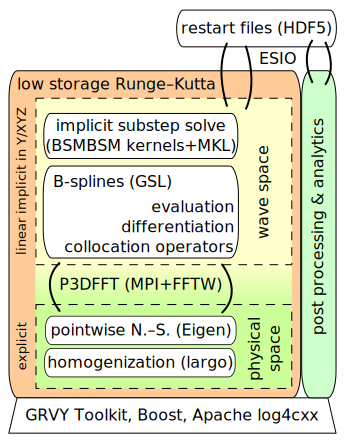
\includegraphics[width=0.6\textwidth]{SuzerainDesignOverview}
\\
\caption{%
    Architecture for the spectral
    simulation framework Suzerain\label{fig:suzeraindesign}
}
\end{figure}

\begin{figure}
\centering
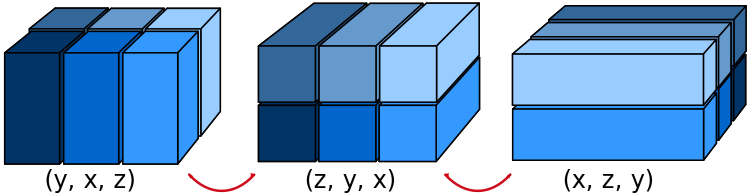
\includegraphics[width=.95\linewidth]{PencilTransposeSchematic}
\\
\caption[Parallel data movement stages for pencil decompositions]{%
  A pencil decomposition maps $O(N^2)$ data to $O(N^3)$ MPI ranks using two
  \texttt{MPI\_Alltoall}-like global communication phases depicted with red
  arrows.  Each color represents the data owned by a single rank in each
  configuration.  \label{fig:penciltranspose}
}
\end{figure}

The high-level design of Suzerain is depicted in \autoref{fig:suzeraindesign}.
Best-of-breed third party libraries were used when it was advantageous to
do so.  Computing one Runge--Kutta substep
per~\eqref{eq:generaloperatormasssubstep} transforms state from wave space to
physical space and transforms residuals back using P3DFFT~\citep{P3DFFTweb}.  These parallel
transposes, depicted in \autoref{fig:penciltranspose}, provide the natural
domain decomposition which arises from the Fourier/B-spline spatial
discretization~\eqref{eq:spatial_discretization}.  The communication and
computation characteristics of those operations are crucial for scalability.

B-spline operators were formed using the GNU Scientific Library
(GSL)~\citep{Eaton2008GNU}.\footnote{%
    The author is a committer for the GSL project.
}
The banded implicit solves in Algorithm~\ref{alg:step} required custom compute
kernels to assemble rescaled B-spline operators into large-bandwidth,
complex-valued BSMBSMs per \autoref{sec:solutionimplicitoperator}.
Factorization and back-substitution are provided by
the Intel\textsuperscript{\textregistered} Math Kernel Library (MKL).\footnote{%
    By default, implicit solves employ a robust, LAPACK-like driver.  The user
    may also choose the vanilla \texttt{GBTRF/GBTRS} pair for speed, the more
    expensive \texttt{GBSVX} driver to monitor operator conditioning, or a
    custom banded driver routine inspired by \citet{Langou2006Exploiting}'s
    \texttt{DGESIRSV} permitting mixed precision operation and/or exploiting
    approximate factorizations.  While this last option provided verifiably
    correct results, reusing the $(k_n,k_m)$-dependent operator (see
    \autoref{fig:discreteimplicitop}) factorization along with iterative
    refinement to avoid nearby $(k_n',k_m')$ factorizations was not found to be
    superior to invoking \texttt{GBTRF} for every $(k_n,k_m)$ on the problems
    considered in this document.
}
Custom banded matrix-vector product kernels were prepared because
compiler-unrolled loops are appreciably faster than general-purpose
MKL routines at small bandwidths~\citep{Lee2013Petascale}.\footnote{%
    Note the matrix-vector product bandwidths are significantly
    smaller than that factorization problem bandwidths as discussed in
    \autoref{sec:solutionimplicitoperator}.
}
In physical space, pointwise
Navier--Stokes-related computations used Eigen~\citep{eigenweb}
to simplify expressing complicated expansions
like~\eqref{eq:linearized_pressure_gradient} and to facilitate accessing
vectorized intrinsics for performance.  When applied, the slow growth forcing
discussed in
Sections~\ref{sec:background_homogenization} and~\ref{sec:imposing_fpg} is
accomplished using largo, a standalone Fortran 90/C99 library developed by Victor
Topalian which is distributed with Suzerain.

The GRVY Toolkit~\citep{GRVYweb} was used for continuous performance monitoring
while extensions atop Apache log4cxx~\citep{log4cxxweb} provided rich, MPI-aware
logging of both application lifecycle events as well as the temporal evolution
of statistical quantities of interest.\footnote{The author is a committer for both
the GRVY Toolkit and Apache log4cxx projects.}  Input and output of
HDF5-based~\citep{hdf5} data files was performed using the
ESIO library~\citep{ESIOweb}, written as part of the current work and also
openly available.\footnote{\url{http://github.com/RhysU/ESIO}}  Operational
considerations like automated batch job output management and reactive tear down
in the event of job time expiration or queue-system-related interruption were
implemented to permit long simulations to run virtually unattended.

Absent from \autoref{fig:suzeraindesign} are the pervasive
computational science toolkits PETSc~\citep{Balay1997Efficient} and
Trilinos~\citep{Heroux2005Overview}.  During Suzerain's early design they were
investigated but six years ago it was unclear how to fit the techniques
from \autoref{sec:techniques} into them.  Three years ago, having learned more,
it became apparent that doing so was possible.  However, at that time, the
basic features either toolkit would have provided had already been long ago
implemented within Suzerain making porting a considerable effort
without immediately obvious benefits.  No port occurred.

In hindsight, not adopting a common toolkit into Suzerain's design was
suboptimal.  Gaining access to off-the-shelf, adaptive temporal schemes
would have permitted taking full advantage of the increased stability provided
by the wavenumber-dependent, linearly implicit operator implementation in the
streamwise and spanwise directions without concerns as to whether or not doing
so adversely impacts accurately capturing turbulent dynamics (see
\autopageref{eq:bigtimesteps} and, below, \autoref{sec:channel_runs}).  It
certainly would have largely rendered the work behind
\autoref{sec:wallnormaleigval} unnecessary as classical CFL stability estimates
would yield conservative initial guesses from which an adaptive scheme could
ramp up the time step to a maximally efficient value given well-quantified
accuracy requirements.  If found prohibitively expensive for production calculations,
adaptive schemes could be applied during simulation ``spin-up'' followed by
nonadaptive time advance using spin-up-informed time step choices.  Reactive
stability restrictions arising from spatiotemporal forcing would have been
seamlessly handled rather than requiring the step size safety factors listed
in \autoref{sec:bldata}.  Finally, and most importantly, skeletally
incorporating a ubiquitous toolkit could increase the likelihood and speed of
future Suzerain adoption by PETSc- or Trilinos-savvy developers thus
facilitating collaboration and providing better research returns for the time
invested in the code.


%%%%%%%%%%%%%%%%%%%%%%%%%%%%%%%%%%%%%%%%%%%%%%%%%%%%%%%%%%%%%%%%%%%%%%%%%%%%%%
\section{Testing and Verification}

Automated testing and code verification are essential as Suzerain is used to
produce data for model calibration.  Unit tests ensure lower level
routines behave as expected while a collection of higher-level tests verify
their proper integration.  MPI-parallel system tests check first for correct operation
and second, wherever applicable, for agreement with serial computations.
Serial/parallel consistency tests include the full application lifecycle
involving loading restart state, advancing time, computing statistics, and
storing state back to disk.  Gold solutions, which are known-correct results
calculated by earlier code revisions, permit detecting when changes
like implementing optimizations or switching compiler versions
unintentionally influence results.
The full test suite
was run daily on a Buildbot continuous integration server~\citep{Buildbot}
against both the GNU and Intel\textsuperscript{\textregistered} compilers.  At present, automated line and function coverage
exceeds 80\%.

%\subsection{The Method of Manufactured Solutions}

To verify that Suzerain correctly implemented Equations~\eqref{eq:nondim_model}, the method of manufactured solutions (MMS)
was employed.  The MMS adds to the governing equations new source
terms such that the exact -- manufactured -- solution is known \textit{a
priori}~\citep{Roache1984Symbolic, Steinberg1985Symbolic, MASA}.  New
manufactured solutions were created to fully test all terms in compressible
Navier--Stokes formulations like the present one~\citep{Ulerich2012MMS}.  The
particular solution instantiation appropriate for the current
nondimensionalization is recorded in Appendix~\ref{sec:mms}.

\begin{figure}[t]
\centering
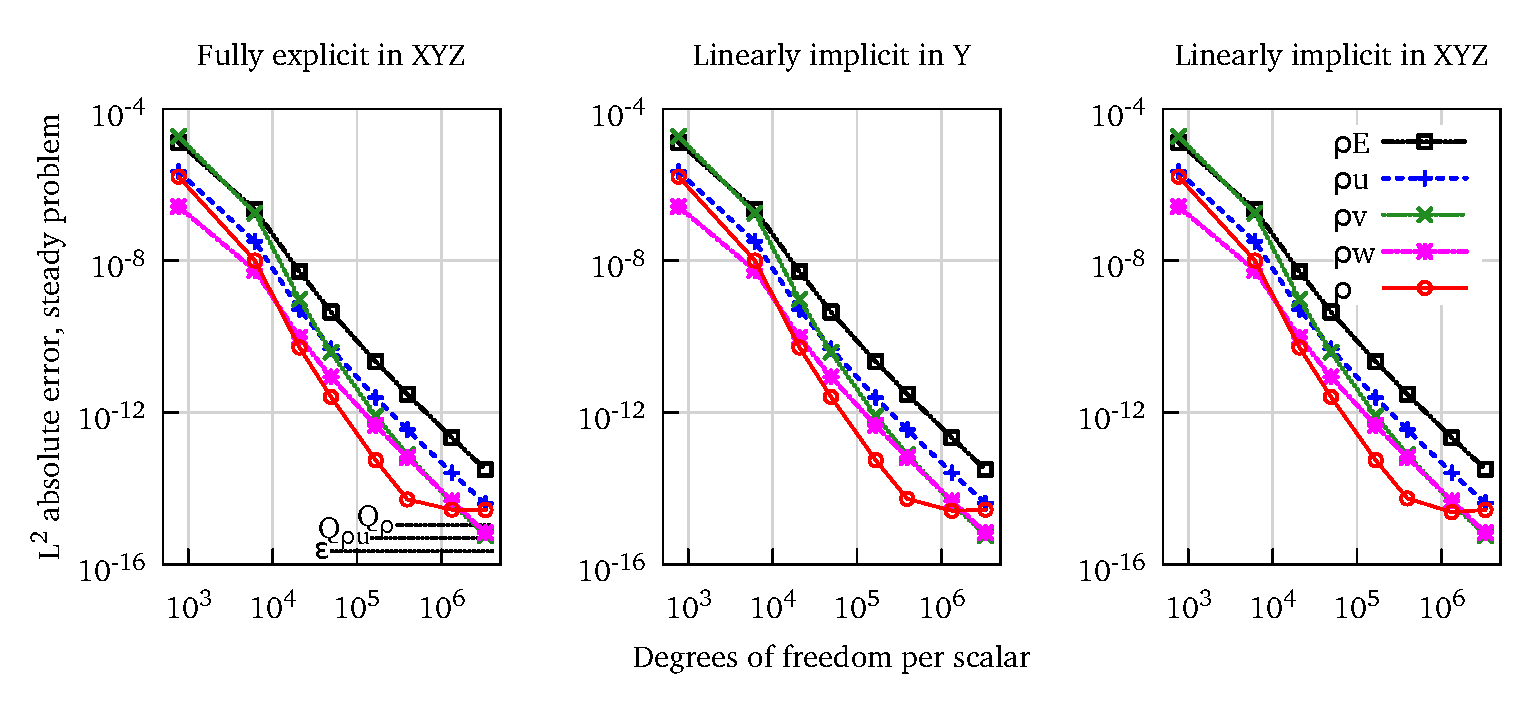
\includegraphics[width=\textwidth]{mms-convergence-steady}
\caption[Verification of Suzerain against a steady manufactured solution]{%
  Convergence behavior against a steady problem solved using each available
  Navier--Stokes operator implementation.  The wall-normal resolution ---
  piecewise-septic B-splines atop uniform breakpoints with 12, 24, 36, 48, 72,
  96, 144, and 192 collocation points --- governs the asymptotic order.  The
  three sample estimate~\eqref{eq:orderest} finds $k_0>7.34$ across $h=48$,
  $h/s=72$, and $h/t=96$ for all scalars.  Labels $Q_\rho$ and $Q_{\rho{}u}$
  indicate measured pointwise error in the floating point computations
  implementing manufactured forcing~\citep{Ulerich2012MMS}.  Beyond 96
  collocation points that forcing error reduces empirical convergence rates.
  For reference, label $\epsilon$ marks machine
  epsilon.\label{fig:convergence-steady}
}
%
\end{figure}

\begin{figure}[t]
\centering
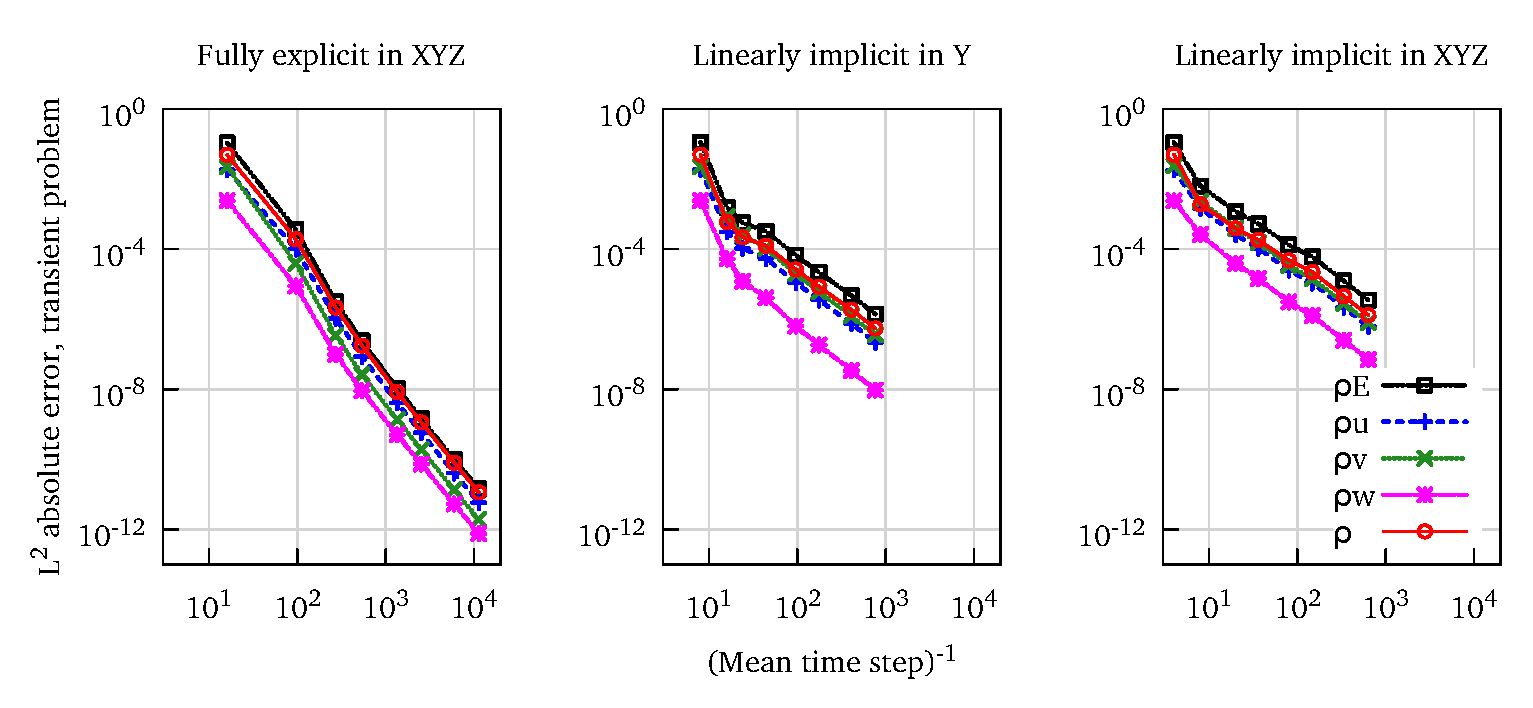
\includegraphics[width=\textwidth]{mms-convergence-transient}
\caption[Verification of Suzerain against a transient manufactured solution]{%
  Convergence behavior against a transient problem over 0.25 time units solved
  using each available Navier--Stokes operator implementation.  The same
  spatial resolutions from \autoref{fig:convergence-steady} were reused to
  force temporal refinement to be driven by stability concerns per
  \autoref{sec:stabilitycriteria}.  When fully explicit (left), stable time
  steps are small enough that pre-asymptotic, almost-spatial orders are
  recovered ($k_0>6.45$).  Wall-normal implicitness (center) exhibits $k_0>3.6$
  for $N_y\geq{}48$ while advancing linearly implicitly in three directions
  (right) shows $k_0>2.1$ for $N_y>72$.  Notice significant differences in
  step sizes occurring across the three
  implementations.\label{fig:convergence-transient}
}
\end{figure}

After the manufactured solution was constructed, three-sample observed order of
accuracy studies were conducted~\citep{Roy2005, Roache1998Verification}.
Assuming an approximation $A(h)$ shows an $h$-dependent truncation
error compared to an exact value $A$, \textit{viz.} $A - A(h) = a_0h^{k_0} +
a_1h^{k_1} + \cdots$, gives rise to the classical Richardson extrapolation
procedure.  Neglecting $O(h^{k_1})$ contributions, one can estimate the leading
error order $k_0$ by numerically solving
\begin{align}
  A &=
  \frac{t^{k_0}A\!\left(\frac{h}{t}\right) - A(h)}{t^{k_0}-1} + O(h^{k_1})
  = \frac{s^{k_0}A\!\left(\frac{h}{s}\right) - A(h)}{s^{k_0}-1} + O(h^{k_1})
  \label{eq:orderest}
\end{align}
given three approximations $A(h)$, $A(h/s)$, and $A(h/t)$ to $A$.  The $L^2$
norm of the absolute error in each scalar field was selected here.  On steady
problems, the wall-normal B-spline discretization error generally dominates that
arising from the spectral streamwise and spanwise Fourier basis truncation as
displayed in \autoref{fig:convergence-steady}.  On transient problems, the
linearly implicit temporal treatment can reduce the asymptotic convergence rate
to as low as second order as demonstrated in
\autoref{fig:convergence-transient}.

\begin{figure}
\centering
\includegraphics[width=\textwidth]{NRBC_rhome_y}
\caption[Verification of nonreflecting boundary conditions]{%
  The temporal evolution of mean pressure across the streamwise and spanwise
  directions as a function of wall-normal distance is depicted during a
  nonreflecting boundary condition test.  At $t=0$ the wall temperature is
  instantaneously dropped causing a pressure pulse to travel towards the upper
  boundary which it exits before $t=5$.  An acceptable reflection is seen
  traveling back towards the wall which it reaches around $t=8$.  The
  effectiveness of the approximately nonreflecting boundary can be contrasted
  with the subsequent pressure reflection from the isothermal wall which is
  faint but visible at $y=5/4$ when $t=10$. \label{fig:nrbc-verify}
}
\end{figure}

Two important code features were not verified via manufactured solutions.  Both
features are, of course, believed to be formulated and implemented correctly but
that belief is not based upon Figures~\ref{fig:convergence-steady}
or~\ref{fig:convergence-transient}.  The first feature was the nonreflecting
boundary treatment discussed in \autoref{sec:nrbc}.  The related
matrix-manipulating logic~\eqref{eq:dimeulertransformevolve_linearfact} was
exercised by automated tests.  A variety of two- and three-dimensional test
problems, like the one depicted in \autoref{fig:nrbc-verify}, were used to
assess proper boundary condition enforcement within the larger temporal
advancement scheme per \eqref{eq:dimeulertransformevolve_nonlinear} and
\eqref{eq:dimeulertransformevolve_linear}.
%
%Empirical reflection coefficients were not, however, assessed.
%
The second feature was the data exchange between the main solver in Suzerain and
the pointwise homogenized forcing computations coded in Topalian's
largo library.  The homogenization-agnostic data hand off between largo and
Suzerain was subjected to intensive code review followed by capturing results in
gold solution files to defend against regression.
%
%It was difficult to provide strong coverage of this code integration point
%without falling prey to excessive brittleness as the slow growth formulations
%evolved within the largo library.
%
Topalian provided automated, pointwise verification of the computations
inside largo.


%%%%%%%%%%%%%%%%%%%%%%%%%%%%%%%%%%%%%%%%%%%%%%%%%%%%%%%%%%%%%%%%%%%%%%%%%%%%%%
\section{Validation on Isothermal Channel Problems}
\label{sec:channel_runs}

To validate Suzerain, including its uncertainty and post-processing
capabilities, a collection of sub- through supersonic, low Reynolds number
isothermal channels was simulated~\citep{Ulerich2012Turbulence}.  The collection
followed computations by \citet{Coleman1995Numerical} which were further
investigated by \citet{Huang1995Compressible} to permit direct comparison with
their results.  A wide range of Mach numbers was simulated to permit investigating, later
in this chapter, the efficiency of the linear-implicit treatment documented in
\autoref{sec:implicitlytreatedterms}.
%
The data is openly archived as described in Appendix~\ref{sec:archiving}.

In channel flows a fluid is driven between two flat plates separated by a fixed
distance as shown in \autoref{fig:geometry}.  The
incompressible~\citep{Kim1987Turbulence, Hoyas2006Scaling, DelAlamo2003Spectra,
DelAlamo2004Scaling, Simens2009Highresolution, Hoyas2008Reynolds} and
compressible~\citep{Coleman1995Numerical, Huang1995Compressible, Li2001DNS,
Morinishi2005Study, Friedrich2007Compressible, Friedrich2004Turbulence,
Lechner2001Turbulent, Schwartz1987Perturbation} versions of this problem are
well-studied.  Half the plate separation distance is taken as reference length
$l_0$ so that nondimensionally $L_y=2$.  No slip, isothermal conditions are
enforced at the upper and lower boundaries.  Unlike the classical plane
Poiseuille flow in which a constant pressure gradient drives the fluid, in
Coleman-like channels the bulk streamwise momentum, $\int\rho{}u\,\mathrm{d}\!y,$
is constrained using a spatially uniform, time-varying body force $f$.  The
instantaneous bulk density is similarly fixed.  In contrast, the total energy is
not constrained so that the problem becomes energetically stationary only when
the mean work done by $f$ is balanced by the average heat transfer through the
walls.  To simplify comparison, the grid resolutions and domain size closely
follow \citet{Coleman1995Numerical} who found them to be adequate.  The domain
is small relative to more recent channels appearing in the
literature.

% Source data from http://turbulence.ices.utexas.edu/coleman/ with MD5:
%   40ded1a60f8d65a7282c5afaa8d43e10  coleman3k01.h5
%   65561dbb6918e828afed9cf31a61f600  coleman3k05.h5
%   73ee5929a5fc4b726e6095ffe1ed2589  coleman3k15.h5
%   f9147b944f908af9b4dfc86b000df89a  coleman3k30.h5
%   1581eee7c8e4ff4a227f67cdf8357235  coleman5k01.h5
%   12658b01075e5acd49098f519fb11918  coleman5k05.h5
%   25d4944b8729aa7308f65302279172fe  coleman5k15.h5
%   5113239ac101f2b7c357fc70f8f49721  coleman5k30.h5

% Number of flow throughs for KMM87 computed as follows:
%    t u_\tau / \delta \approx 10 (page 140 second to last paragraph)
%    \delta = 1
%    U_m / u_\tau = 15.63 (Table 1)
%    U_m = 1
%    L_x = 4*pi*\delta
% combining shows 12.43 flow throughs

\begin{table}
\makecommand{\z}{\phantom{0}}  % Facilitates column alignment
\makecommand{\Z}{\phantom{.0}} % Ditto
\centering
\caption[Isothermal channel simulations]{%
    Isothermal channel simulations performed with Suzerain
    v0.1.6.34-r45407.  For all cases, $\overline{\rho} = 1$,
    $\overline{\rho{} u} = 1$, $T_w = 1$, $\textrm{Pr} = \mu C_p
    / \kappa = 0.7$, $\alpha=0$ for $\mu_B=\alpha\mu$, $\mu /
    \mu_0={\left(T / T_0\right)}^\beta$, and $\gamma = C_p / C_v =
    1.4$.  Extents were $L_x=4\pi$, $L_y=2$, $L_z=4\pi/3$ employing
    $N_x=192$ and $N_z=168$ Fourier modes and a piecewise-septic
    B-spline basis with $N_y$ collocation points stretched per
    the hyperbolic tangent parameter ``$\tanh$'' following~\eqref{eq:htstretch2}.  By definition,
    $\textrm{Re} = \overline{\rho{}u}\left(L_y / 2\right) / \mu_w$,
    $\textrm{Ma} = \bar{u} / a_w$.  Simulations by
    \citet*{Kim1987Turbulence} and \citet*{Coleman1995Numerical} are
    shown for comparison.\label{tbl:table_channel}
}
{\renewcommand{\tabcolsep}{0.435em}
\begin{tabular}{cccccccccccr}
Case                                     & % Simulation input parameters
$\textrm{Re}$                            &
$\textrm{Ma}$                            &
$\beta$                                  &
$N_y$                                    &
$\tanh$                                  &
$\textrm{Re}_\tau$                       & % Details from post-processing
$\Delta{}x^{+}$                          &
$y_{1}^{+}$                              &
$y_{10}^{+}$                             &
$\Delta{}z^{+}$                          &
\shortstack[c]{Flow\\throughs}
\\
\toprule\toprule
%id       &  Re    &  Ma    &  beta  &  Ny     &  tanh  &  Re &  x+    &  y+1   & y+10  &  z+   &   Flowthroughs       \\
c03k01    &  3000  &  0.1   &  \nicefrac{2}{3} &  128  &  2.25  & 191 &  12.5  &  0.22  & 11.9  & \z5.0 &   15.6       \\
c03k05    &  3000  &  0.5   &  \nicefrac{2}{3} &  128  &  2.25  & 194 &  12.7  &  0.22  & 12.1  & \z5.1 &   15.7       \\
\rowcolor{yellow}
c03k15    &  3000  &  1.5   &  \nicefrac{2}{3} &  128  &  2.25  & 222 &  14.6  &  0.26  & 13.8  & \z5.8 &   11.9       \\
c03k30    &  3000  &  3.0   &  \nicefrac{2}{3} &  128  &  2.25  & 297 &  19.4  &  0.34  & 18.5  & \z7.8 &   15.5       \\
\midrule
c05k01    &  5000  &  0.1   &  \nicefrac{2}{3} &  144  &  2.50  & 298 &  19.5  &  0.26  & 14.2  & \z7.8 &   11.1       \\
c05k05    &  5000  &  0.5   &  \nicefrac{2}{3} &  144  &  2.50  & 303 &  19.8  &  0.26  & 14.4  & \z7.9 &   11.6       \\
c05k15    &  5000  &  1.5   &  \nicefrac{2}{3} &  144  &  2.50  & 349 &  22.8  &  0.31  & 16.6  & \z9.1 &   13.2       \\
c05k30    &  5000  &  3.0   &  \nicefrac{2}{3} &  144  &  2.50  & 480 &  31.4  &  0.42  & 22.8  & 12.6  &   12.9       \\
\midrule
KMM87     &  2800  &  0\Z   &  0\Z             &  129  &        & 180 &  12\Z  &  0.05  & \z5.4 & \z7\Z &   12.4       \\
\rowcolor{yellow}
CKM95a    &  3000  &  1.5   &  0.7             &  119  &        & 222 &  17\Z  &  0.1\z & \z8\Z & 10\Z  &  $\geq 11.9$ \\
CKM95b    &  4880  &  3.0   &  0.7             &  119  &        & 451 &  39\Z  &  0.2\z & 17\Z  & 24\Z  &  $\geq 11.9$
\end{tabular}}
%
\\\vspace*{1.75em}
%
\begin{tabular}{cccccccccc}
Case                            &
$\textrm{Ma}_c$                 &
$\textrm{Ma}_\tau$              &
$\textrm{Re}_c$                 &
$y^\ast_c$                      &
$-\textrm{B}_q$                 &
${\rho}_w$                      &
${\rho}_c$                      &
${T}_c$                         &
${\mu}_c$
\\
\toprule\toprule
%id     &  Mac     &  Matau   &  Rec   &  {y*c} &  -Bq     &  rhow    &  rhoc    &  Tc      &  muc     \\
c03k01  &  0.116   &  0.006   &  3481  &  190   &  0.0003  &  1.002   &  0.9999  &  1.002   &  1.001   \\
c03k05  &  0.570   &  0.031   &  3387  &  185   &  0.0062  &  1.040   &  0.9973  &  1.043   &  1.028   \\
\rowcolor{yellow}
c03k15  &  1.497   &  0.081   &  2772  &  151   &  0.0496  &  1.365   &  0.9780  &  1.391   &  1.246   \\
c03k30  &  2.240   &  0.119   &  1765  &  \z94  &  0.1486  &  2.494   &  0.9278  &  2.666   &  1.923   \\
\midrule
c05k01  &  0.115   &  0.006   &  5752  &  297   &  0.0002  &  1.002   &  0.9999  &  1.002   &  1.001   \\
c05k05  &  0.566   &  0.029   &  5606  &  288   &  0.0058  &  1.041   &  0.9979  &  1.042   &  1.028   \\
c05k15  &  1.477   &  0.077   &  4585  &  238   &  0.0464  &  1.366   &  0.9835  &  1.385   &  1.242   \\
c05k30  &  2.202   &  0.116   &  2974  &  157   &  0.1436  &  2.486   &  0.9500  &  2.598   &  1.890   \\
\midrule
KMM87   &  0\Z\z\z &  0\Z\z\z &  3300  &  180   &  0\Z\z\z &  1\Z\z\z &  1\Z\z\z &  1\Z\z\z &  1\Z\z\z \\
\rowcolor{yellow}
CKM95a  &  1.502   &  0.082   &  2760  &  151   &  0.049   &  1.355   &  0.980   &  1.378   &  1.252   \\
CKM95b  &  2.225   &  0.116   &  2872  &  150   &  0.137   &  2.388   &  0.952   &  2.490   &  1.894
\end{tabular}
\end{table}

%
The channels simulated, including resolution details and various quantities of
interest, are reported in \autoref{tbl:table_channel}.  In the table, wall and
centerline quantities have subscripts $w$ and $c$.  Superscript ${+}$ denotes
normalization by the viscous length scale $\delta_\nu = \mu_w / \rho_w / u_\tau$ or the friction
velocity $u_\tau = \sqrt{\tau_w / \rho_w}$ where the wall shear stress
$\tau_w = \left(\mu \partial_y u\right)_w$.  The friction Reynolds number
$\Reynolds[\tau]{}$ and friction Mach number $\Mach[\tau]{}$ are given by
$y_c/\delta_\nu$ and $u_\tau/a_w$.  Superscript $\ast$ marks
scaling by semi-local units
%
using either $u^\ast_\tau = \sqrt{\tau_w / \rho}$ or $\delta^\ast_\nu = \nu / u^\ast_\tau$~\citep{Huang1995Compressible,Morinishi2005Study}.
%which are similar to
%$\delta_\nu$ and $u_\tau$ except that local density and viscosity are used in
%lieu of wall values.
The nondimensional heat flux is denoted by
$B_q$~\citep{Bradshaw1977Compressible}.  The column ``flow throughs'' conveys
the time over which the data ensemble was collected, divided by the time required
for the bulk flow to traverse the streamwise extent of the domain.
Linearly implicit operators were used in all three directions.

A direct comparison between the present results and those by
\citet{Coleman1995Numerical} can be made from the $\Reynolds=3000$, $\Mach=1.5$
cases c03k15 and CKM95a, which are highlighted in \autoref{tbl:table_channel}.
Aside from differences in the numerics,\footnote{%
    \citeauthor{Coleman1995Numerical} used a Fourier-Legendre spatial
    discretization and a third-order, four-substep temporal scheme
    by \citet{Buell1990Direct}.
}
in the upper half of the table the only appreciable parameter differences
between these two cases are the wall normal resolution ($\Delta{}y^{+}_{10}$ of
$13.8$ vs $8$) and the viscosity power law exponent ($\beta$ of $2/3$ versus
$0.7$).  One-dimensional Fourier spectra at $y\approx{}0.04$ and $y\approx{}1$
(not shown) compare favorably indicating the former difference is benign.  The
latter difference was deliberate as it produces data mildly more appropriate for
high temperature environments as demonstrated by \autoref{fig:Svehla1962}.  In
the lower half of the table, discrepancies between these two particular
simulations range from $0.43\%$ ($\Reynolds[c]{}$) to $1.3\%$ ($\Mach[\tau]$).
Minor disagreement is expected per the noted parameter differences but
additional root causes are further explored below.  Though nominally possible,
another comparison between rows c05k30 and CKM95b is not valid as the c05k30
hyperbolic tangent stretching parameter was too small causing insufficient
near-wall resolution as assessed by spectra (not shown).

%\begin{figure}
%\centering
%\includegraphics[width=0.495\textwidth]{c03k15_figure7a}
%\hfill
%\includegraphics[width=0.495\textwidth]{ckm95_figure7a}
%\\
%\caption[Isothermal channel profile comparison at $\Reynolds=3000$, $Mach=1.5$]{%
%  Comparison of mean primitive quantity profiles from present simulation c03k15 (left)
%  and CKM95a (right), reproduced from \citet{Coleman1995Numerical}.
%  \label{fig:qual_r3km15_comp}
%}
%\end{figure}

\begin{figure}
\centering
\includegraphics[width=\textwidth]{profile-c03k15}
\caption[Profiles with quantified uncertainty for $\Reynolds=3000$, $\Mach=1.5$ channel]{%
    Reynolds-averaged primitive profiles (upper left) and Favre-averaged
    Reynolds stresses scaled by semi-local units~\citep{Huang1995Compressible}
    (lower left) with estimated standard errors as a fraction of mean (upper
    right, lower right) from simulation c03k15.\label{fig:basic3k15}
    % COMPARE ColemanJFM1995 Figure 7a
}
\end{figure}

Based on techniques from \autoref{eq:uqaccounting}, mean primitive quantity and
Favre-averaged Reynolds stress profiles along with pointwise uncertainty
estimates appear for simulation c03k15 in \autoref{fig:basic3k15}.  The
autoregressive technique by \citet{Oliver2014Estimating} was used to estimate
pointwise sampling error at each wall-normal collocation point based on 383
instantaneous averages over the two Fourier directions.  In the upper right of
the figure, uncertainties normalized by mean velocity $\bar{u}$, temperature
$\bar{T}$, and viscosity $\bar{\mu}$ are higher near the wall due to both
turbulent fluctuations and the fact that the mean values take minima there.  The
largest normalized uncertainties in mean density $\bar{\rho}$ are slightly
offset from the other peaks because the mean value increases as one approaches the wall.  Uncertainty
in $\bar{u}$ is appreciably larger than that for the thermodynamic quantities
consistent with their relative root-mean-squared magnitudes \citep[Figures~10
and~18]{Coleman1995Numerical}.
%
We were unable to locate a published uncertainty estimate by Coleman or his
collaborators for the CKM95a simulation data against which to compare.
%
Uncertainty in near-wall $\bar{u}$ and centerline $\bar{u}$ are roughly 6 and
1.5 times larger, respectively, than analogous incompressible results from
\citet{Oliver2014Estimating} when both are scaled by the inverse root of the
number of flow throughs in the ensemble.  This difference will be addressed in
more detail below.

In the lower right of the figure, sampling errors have been propagated into the
derived, Favre-averaged quantities via the Taylor series
method~\eqref{eq:tsm_var1}.  Uncertainty in the density-weighted Reynolds
stresses is approximately an order of magnitude higher than was found for
quantities like $\bar{u}$.  The stresses are partially less certain because
their calculation takes as input higher order moments which are inherently less
well-known given a finite sampling window.  A second factor contributing to
uncertainty in the stresses is that the definition of
$\widetilde{u_i^{\prime\prime}u_j^{\prime\prime}}$ involves scaling by
$\bar{\rho}^{-1}$ which magnifies uncertainty when applying the Taylor
expansion~\eqref{eq:tsm_var1}.

A third factor contributing to relatively higher uncertainties in the Reynolds
stress was an operational error.  It was discovered because the \emph{a
posteriori} uncertainty estimates showed larger-than-anticipated asymmetries
about the channel centerline though mean values did not.
%
Given the solver verification results in \autoref{fig:convergence-steady} and
\autoref{fig:convergence-transient}, an error in the implementation of the
post-processing logic initially was suspected but no symmetry-breaking issues
were uncovered there.
%
On careful review, all new simulations in \autoref{tbl:table_channel} showed
evidence of infrequent, mild near-wall temporal instability though they used
the empirical B-spline operator stability estimates
with the safety factor
of 0.72.
%
The problem was diagnosed from temporal traces of the instantaneous global
minimum of the streamwise momentum--- a simulation monitoring feature not yet
implemented when the empirical stability estimates were created.  Channel flows
exhibit small, pointwise-negative velocities near the wall and it is exactly
these locations where linear-implicitness about the instantaneous mean state,
as described in \autoref{sec:implicitlytreatedterms}, is most subject to
stability problems when time steps are too large.
%
Implicit treatment in only the wall-normal direction also showed, under review,
the same symptom indicating that the operator stability estimates from
\autoref{sec:wallnormaleigval} were too aggressive for the safety factor
0.72.\todo{Sane threshold was 0.40 for c03k15}

Marginal temporal instability was manifest in asymmetric uncertainty estimates
because independent, short-duration instability events occurred infrequently
enough near each wall that over O(10) flow throughs in a small domain their
impact was not distributed evenly between the upper and lower halves of the
channel.
%
As a consequence of this mistake, figures in the present section do not merge
the upper and lower portions of the channel as is commonly done.  Not merging
data across the centerline accounts for a factor of 1.5 increase in $\bar{u}$
uncertainty relative to aforementioned scaled results by
\citet{Oliver2014Estimating}.
%
The remaining threefold increase in near-wall $\bar{u}$ uncertainty relative to
their work is at least partially due to these infrequent events.  That said,
it is also partially attributed to the growth in root-mean-squared $u$
fluctuations as the Mach number increases.
%
The same time step size mistake certainly contributes to the disagreement
between cases c03k15 and CKM95a found in \autoref{tbl:table_channel} and the
jaggedness of the near-wall uncertainty curves in the upper right of
\autoref{fig:basic3k15}.

\begin{figure}[tb]
\centering
\includegraphics[width=0.85\textwidth]{tke3k15}
\caption[Turbulent kinetic energy budgets for $\Reynolds=3000$, $\Mach=1.5$ channel]{%
    Budgets for the turbulent kinetic energy~\eqref{eq:fans_tke}
    for channel simulation c03k15 normalized as by~\citet[figure
    16a]{Huang1995Compressible}.  Omitted terms relative
    to~\eqref{eq:fans_tke} are a factor of 25 times smaller than maximum
    production.~\cite{Guarini2000Direct}\label{fig:tke3k15}.
    % COMPARE HuangJFM1995 Figure 16
}
\end{figure}

Term-by-term budgets for the turbulent kinetic energy~\eqref{eq:fans_tke}
in \autoref{fig:tke3k15} support the conclusion that time
discretization errors are appreciable in simulation c03k15.  Qualitatively, all
terms show expected trends.  However, relative to \citet[Figure
16a]{Huang1995Compressible}, approximately 5\% too much turbulent dissipation,
$\bar{\rho}\epsilon/\Reynolds$, is present at the wall along with a
counterbalancing increase in turbulent work.  \citet{Coleman2010Primer} linked
increased dissipation with temporal inaccuracy when Runge--Kutta schemes are
used.  Other terms are similarly affected.  For example, peak production $-\bar{\rho}
\widetilde{u^{\prime\prime}\otimes{}u^{\prime\prime}} : \nabla\tilde{u}$ is
roughly 10\% lower than \citeauthor{Huang1995Compressible} reported.
However, Suzerain's post-processing logic and the overall budget balance
are sound because the pointwise turbulent kinetic energy equation residual,
is appropriately small.


%%%%%%%%%%%%%%%%%%%%%%%%%%%%%%%%%%%%%%%%%%%%%%%%%%%%%%%%%%%%%%%%%%%%%%%%%%%%%%
\section{Performance and Scalability}
\label{sec:performance}

This section first discusses the efficiency of three available Navier--Stokes
operator implementations, briefly compares Suzerain's performance against a
highly tuned incompressible channel code, and lastly examines Suzerain's
scalability on production homogenized boundary layer simulations.  All
performance measurements were made on the Lonestar4 supercomputer at the Texas
Advanced Computing Center (TACC) as it will be the resource used for
production simulations in subsequent chapters.  Each compute node on Lonestar
contains 2~hex-core Intel\textsuperscript{\textregistered} Xeon\textsuperscript{\textregistered}~5680 3.33~GHz
processors and 24~GB of DDR3-1333~MHz memory.  Every core was used as a separate
MPI rank as Suzerain presently is not OpenMP-enabled.  Compute nodes are
interconnected in a fat-tree topology using Mellanox\textsuperscript{\textregistered}
InfiniBand\textsuperscript{\texttrademark} switches running at quad data rates of 40~Gbits/second.
Compilation was performed with version 11.1 20101201 of the
Intel\textsuperscript{\textregistered} compilers at optimization level~3 with host-specific
extensions enabled.

The efficiency of the fully explicit, linearly implicit in the wall-normal
direction, and linearly implicit in three directions operators were benchmarked
and are reported in \autoref{tbl:channel_performance}.  Efficiency was
measured as the amount of wall time required to advance one nondimensional time
unit because that physics-oriented metric directly translates into the expense
of acquiring converged turbulence statistics.  Another metric, wall time per
time step, will be presented later alongside scalability results.  Centerline
Mach numbers across the eight cases considered vary by nearly a factor of
twenty.   This broad range permits assessing efficiency for widely varying
acoustic-versus-convective restrictions as well as significant differences in
thermodynamic property fluctuation magnitudes.

\begin{table}
\centering
\makecommand{\z}{\phantom{0}}  % Facilitates column alignment
\caption[Relative efficiency of the Navier--Stokes operator implementations]{%
    Normalized wall time to advance simulation one nondimensional time unit
    using each of the available Navier--Stokes operator implementations.  Cases,
    defined in \autoref{tbl:table_channel}, were executed with Suzerain
    v0.1.6.34-r45407 using 12 nodes of Lonestar4.\label{tbl:channel_performance}
}
\begin{tabular}{cccc}
Case &
\shortstack[c]{Linearly implicit\\XYZ} &
\shortstack[c]{Linearly implicit\\Wall-normal} &
\shortstack[c]{Fully explicit}
\\
\toprule\toprule
%id     &  rhome_xyz  &  rhome_y  &  explicit
c03k01  &  \z1.0      &  11.0     &  49.5   \\
c03k05  &  \z1.0      &  \z2.9    &  10.3   \\
c03k15  &  \z1.0      &  \z1.3    &  \z3.7  \\
c03k30  &  \z1.0      &  \z1.4    &  \z2.0  \\
\midrule
c05k01  &  \z1.0      &  \z8.7    &  48.7   \\
c05k05  &  \z1.0      &  \z2.5    &  10.4   \\
c05k15  &  \z1.0      &  \z1.7    &  \z4.4  \\
c05k30  &  \z1.0      &  \z1.3    &  \z2.3  \\
\end{tabular}
\end{table}

On the eight cases examined, linear implicitness in three directions produced
time to solution speedups of 1.3--11x relative to treating only the wall-normal
direction implicitly.  The speedup improved as the Mach number decreased because
the more implicit operator mitigates streamwise and spanwise acoustic stability
concerns that would otherwise dominate at those conditions.  The measurable
speedup in higher speed channels is perhaps counterintuitive as the more
implicit
implementation requires matrix assembly and factorization for every $(k_m, k_n)$
wavenumber pair while the second fastest does not.  Though factorization has a
much higher asymptotic complexity than assembly, at this resolution the former
takes only twice the wall time of the latter.  Factorization of the assembled
matrices, here possessing bandwidth 69, has a favorable memory access pattern in
contrast with the assembly kernels and consequently performs comparatively well
despite the larger number of floating point operations it requires.
%
%%One additional benefit of increased implicitness is that it reduces
%%the number of \texttt{MPI\_Alltoall}-like parallel communication phases
%%required per simulation time unit during which no useful computations
%%are performed.

The above conclusions are what prompted selecting implicitness in three
directions for the isothermal channel simulations discussed in the prior
section.  Note that though less aggressive time step safety factors than 0.72
were in that section concluded to be required, safety factor reductions impact both
available implicit treatments fairly equitably and therefore do not grossly
upset their relative efficiencies.  Some simulations performed as part of the
next two chapters will use only wall-normal implicitness because they were not
limited by streamwise or spanwise stability thus making wavenumber-dependent
linear algebra detrimental to time-to-solution efficiency.  In summary, having both
types of implicitness available in Suzerain as equally viable options permits
the code to effectively address the wide range of flow conditions studied.

To assess the performance of Suzerain as a direct numerical simulation
framework, we compared it against the highly optimized channel
code PoongBack~\citep{Lee2013Petascale, Lee2014Experiences}, written by
Myoungkyu Lee.  PoongBack is a comparatively monolithic Fortran code for solving
the incompressible Navier--Stokes equations.  Like
Suzerain, PoongBack uses a Fourier--Galerkin/B-spline collocation spatial
representation in conjunction with a three-stage, low-storage semi-implicit
advance.  The \citet{Kim1987Turbulence} Navier--Stokes formulation advances two scalar state
variables in time requiring three wave-to-physical parallel Fourier transforms
and five physical-to-wave transforms per time step.  Every $(k_m, k_n)$
wavenumber pair requires multiple linear solves but the operators do not couple
multiple equations and require relatively uncomplicated matrix assembly to form.
Unlike Suzerain, PoongBack uses wholly custom linear algebra routines,
wholly custom, quadrature-aware parallel Fourier transforms built atop FFTW
3.3's MPI capabilities, and hybrid MPI/OpenMP parallelism.  The comparison is
apt because many of Lee's improvements could be adopted by Suzerain if
performance improvements are required for future work.

Mimicking the resolution from our simulation c03k01, Lee
performed an $\Reynolds[\tau]=180$ simulation on 12 nodes of Lonestar4 using 6
OpenMP threads per processor.  PoongBack took 0.1299 seconds to complete one
Runge--Kutta step.  The timing of high-level tasks from our c03k01 case were
collected and then scaled by the frequency with which they are required to
advance the \citet{Kim1987Turbulence} formulation.  For example,
the wall time P3DFFT required to transform 30+ scalar fields from wave space to
physical space was scaled to reflect PoongBack only needing to perform that task
for three fields.
%
Physical space nonlinear product costs were scaled by the ratio of the number of
scalar equations involved, a conservative choice because the incompressible
system of equations is considerably less complex than the
compressible one.
%
% Comparing notes with MK on 2 July 2014
%
% Code      Operation Number/Substep Complexity
% Suzerain  Factorize 1              S**3
%           Backsub   1              S**2
%           Matvec    33             1
%           Assembly  1              S**2
%           Wave2Phys 33             1
%           Phys2Wave 4 (channel)    1
%           Nonlinear 1              5
% PoongBack Factorize 6              S**1
%           Backsub   29             1
%           Matvec    41             1
%           Assembly  2              1
%           Wave2Phys 3              1
%           Phys2Wave 5              1
%           Nonlinear 1              2
%
Scaling for linear algebra tasks, including matrix-vector products, matrix
assembly, back substitution, and factorization, reflected both the relative
number of tasks performed during one substep as well as relative code-to-code
operation costs arising from differences in equation coupling.  For example,
factorization costs were scaled by $6/5^3$ as, per wavenumber pair, PoongBack
performs six single-equation factorizations while Suzerain performs one
monolithic factorization with a leading-order, \texttt{S}-dependent cubic
complexity~\eqref{eq:bsmbsm_factorization}.

After rescaling, each hypothetical
Suzerain time step solving the incompressible \citeauthor{Kim1987Turbulence}
formulation required 0.629 seconds representing a 4.8x slowdown relative to
PoongBack.  About 30\% of the hypothetical wall time per time step would be
spent on parallel transposes with the vast majority of the remainder consumed by
banded algebraic operations.  Less conservative estimates of the nonlinear
product costs incurred in physical space bring the hypothetical slowdown as low
as $4\times$.  The hypothetical slowdown is larger than hoped but reasonable---
Lee took in excess of a year to produce PoongBack with much of that time spent
crafting and tuning formulation-specific banded algebraic logic to which he
attributes an overall speedup of $2\times$ (personal communication).

% State:  512x256x256 by 5 fields by 8 bytes per double
% Padded: 768x256x384 by 33(down)+5(up) fields across 3 substeps by 8 bytes
%
Suzerain's strong scalability as well as timings for the three available
Navier--Stokes operator implementations are shown in \autoref{fig:scaling}.
The problem size studied, which could run on as few as 24 MPI ranks,
corresponds to the production grid to appear in \autoref{sec:bldata}.  The state
is only 168 million real-valued degrees of freedom (1.3~GB) but each
full Runge--Kutta step required P3DFFT to transmit and fast Fourier
transform 69~GB of information.  Scalability from 24 to 48 ranks was not
good but from 48 to 384 ranks operator-specific parallel efficiencies
exceeded 93.3\%.  Within this sweet spot, advancing linear implicitly in
one or three directions took 107--110\% or 152--155\% of the wall time
of a fully explicit time step, respectively.

\begin{figure}[tb]
\centering
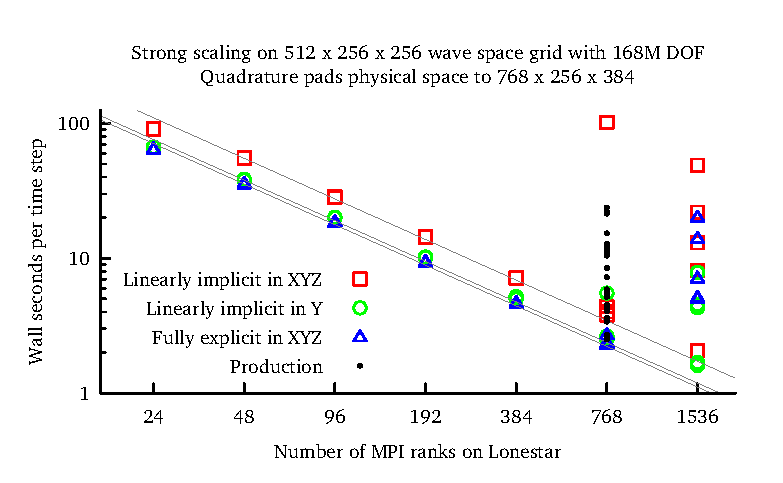
\includegraphics[width=0.85\textwidth]{scaling}
\caption[Strong scalability of Suzerain on TACC's Lonestar4 resource]{%
    Strong scalability on a homogenized boundary layer scenario.  At least three
    samples are present for each rank count and Navier--Stokes operator
    implementation.  Workload is well-balanced at all rank counts.
    Grey lines indicate perfect parallel efficiency based upon 48-rank
    performance.  Production timings, here implicit in only the
    wall-normal direction, included the overhead of writing statistics and
    checkpoint files.\label{fig:scaling}
}
\end{figure}


At 768 and 1536 ranks, job-to-job measurements of the wall seconds per time step
became highly variable.  We attribute the behavior either to such batch jobs
often executing on compute nodes separated widely on Lonestar4's fat-tree
interconnect or to some other intermittent network issue.  Though some
variability was always present at these rank counts, atop an unchanged Suzerain
binary it became dramatically worse after a Lonestar4 system maintenance on 27
May 2014.  The better jobs measured after that date exhibited coefficients of
variation between 2--4\% for the time it took P3DFFT to transform a single
scalar field while the worse jobs exceeded 500\%.  P3DFFT scalability problems
on Lonestar4 at 768 and 1536 ranks was also observed by \citet{Lee2013Petascale}
though they encountered nothing so severe.  Despite these issues and due to
time-to-solution considerations, production simulations were executed on 768
ranks because, when provided with a favorable network fragment, job efficiency
moving from 384 to 768 ranks could approach 100\%.  \autoref{fig:scaling}
includes laggard production jobs that, when detected, were manually stopped to
conserve compute resources.

%%As mentioned, the problem decomposition provided by the parallel transpose
%%library dictates scalability.  Balancing communication and computation tradeoffs
%%in conjunction with resolution requirements can be difficult and lead to
%%suboptimal scaling as above.  One promising approach, now deployed in a
%%hero-class, incompressible DNS code by \citet{Lee2013Petascale}, is adding
%%on-rank parallelism using OpenMP as well as FFTW's OpenMP-aware, autotuned
%%parallel transposes.  Hybrid parallelism allows greater flexibility in mapping
%%workloads to increasingly common many-core compute nodes.  An alternative
%%transpose library to P3DFFT, called ``underling'' and written as part of this
%%work, will allow seamlessly taking advantage of FFTW MPI's autotuned
%%capabilities~\citep{Frigo2005Design}.

%%Lastly, preliminary numerical analysis suggests that taking linearization
%%references about maximum rather than mean kinematic viscosities may
%%provide additional diffusive stability.  This analysis is to be hardened
%%and implemented as well.


\chapter{Validation}

%\section{Calibration and Validation}
%\section{Validation}
\label{sec:validation}

% VALIDATION TODO
%
% show major effort
% table of results
% show hierarchy
% precisely define cases 
%
%

%
% meshed vanes are 24x more expensive
%

The previous chapters briefly outlined the physical phenomenon under
consideration, the mathematical models proposed to simulate it,
and the numerical solution of these models for a variety of system 
configurations and scenarios. Before these simulations can be used 
as a tool to evaluate proposed system designs, it is necessary to
validate that the physical model in use accurately represent
reality. As defined by Moser et al.\cite{Moser2012Validating},
``validation is the process of determining whether a mathematical model
is a sufficient representation of reality for the purposes for which the
model will be used--that is, for predicting specified QoIs (Quantities
of Interest) to inform a specific decision.'' 

This chapter contains a discussion of the validation of the
computational models against existing experimental data and high
fidelity simulations. This chapter does not exhaustively detail the
validation studies performed in the course of this study. Rather, this
chapter discusses four representative cases and the overall validation
approach pursued. A more detailed set of validation data is provided in 
Appendix~\ref{app-validation}. The limited validation that was performed
for the 2016 field tests in discussed in Chapter~\ref{sec:field}. 

A challenge in this project is the scarcity of experimental data. Only
two or three cases of experimental measurements are available. These
measurements, for reasons detailed in the next section, are not
sufficient to provide confidence in the output of simulations across a
wide variety  of scenarios. Therefore, a high fidelity model using 
meshed vanes with enforced no-slip velocity boundary conditions along
the surface of the vane was developed. These ``gridded'' runs have
been validated against the experimental data, which they match quite
closely. However, as detailed in Chapter~\ref{subsec:vane}, 
explicitly meshing the vanes would be far too 
prohibitively expensive to permit a rapid exploration of a variety of
system configurations. Instead, this high fidelity model is used 
to generate additional reliable data to permit validation of lower
fidelity models, such as the virtual vanes. Likewise, the results of the
unsteady virtual vane simulations can be used as validation data for a
further reduced, steady Navier-Stokes model. This hierarchy of
validation is shown in Figure~\ref{fig:val_hier}, with data sources that
generate more reliable data at the top, and models that are less
reliable, but also less computationally expensive at the bottom. In
terms of expense, the steady virtual vane model generates a solution in
approximately two minutes, versus twelve hours for the unsteady virtual
vane model. The gridded vanes require another factor of ten in
computational time, and many more man-hours hours of work to generate
the mesh. Therefore, it is unrealistic to perform parameter sweeps or
system configuration investigations with the gridded vanes and these
results are used only for validation studies. Instead, the
steady model is used, with promising results re-evaluated with unsteady
virtual vane models. %and so on up the hierarchy if more confidence is necessary. 

%
% https://www.draw.io/
%
 \begin{figure}[!htb]
   \begin{center}
    \includegraphics[width = 8 cm]{figs/validation_hierarchy}
    \caption{This figure depicts the validation hierarchy. The
    experimental measurements are at the top, where the data is expected
    to be the most reliable, but simultaneously the most
    limited. Moving down the table leads to simulated data sources that
    are less reliable but increasingly cheaper in time to generate. At
    the bottom is the reduced order model from steady virtual vane solutions.} 
    \label{fig:val_hier}
   \end{center}
 \end{figure}

Three kinds of experimental validation data are available. These are
data generated in the laboratory using a heated plate, data from
experiments in the wind tunnel (``Wind-only''), and measurements from field
tests (``Field'') conducted in Arizona. The available data from
these cases and the gridded vanes created to mimic them are are
summarized in Table~\ref{tab:val_data}. Every case shown has been
simulated using the virtual vanes.   

%\large
\begin{table}[h]
\centering
\label{my-label}
\begin{tabular}{l|l|l|l|}
           & Wind-Only                   & Thermal-Only                & Field  \\
  \hline 
Experiment & Straight Vanes $60^{\circ}$ & Straight Vanes $60^{\circ}$ & June 2014   \\
           &                           & Straight Vanes $30^{\circ}$   & August 2014 \\
           &                           & Hybrid (Two tier)             & August 2015 \\
  \hline 
Gridded    & Straight Vanes $60^{\circ}$ & Straight Vanes $60^{\circ}$ & \\
           & Straight Vanes $30^{\circ}$ & Straight Vanes $30^{\circ}$ & \\
  \hline 
\end{tabular}
  \caption{Available truth data from the laboratory experiments 
    (cold wind and thermal-only), the field tests, and the gridded
 vanes.}  
  \label{tab:val_data}
\end{table}
%
%
%
% http://www.tablesgenerator.com/
%
%


%
% experimental challenges
%
%\normalsize
\section{Thermal-Only Validation}
This section provides examples of the validation performed with the
richest data set, the measurements in the laboratory. All of the
thermal-only the data was generated in a laboratory setting at Georgia
Tech. The general system configuration is depicted in Figure
\ref{fig:lab_image}. These data were taken using stereo particle image
velocimetery (PIV) at Georgia Tech by Mark Simpson and Ari Glezer, and
the errors in in measurement and sampling are 
not quoted. The particles are seeded outside of the array vanes and
permitted to naturally convect into the turning vane enclosure. The
particles were from a glycol-water theatrical fog (Rosco Fog Fluid). 
Only velocity measurements are available. Several
potentially important quantities of interest, such as the pressure and
temperature, have not been measured. 

%
% http://convertonlinefree.com/ConvertImageEN.aspx
%
 \begin{figure}[!htb]
   \begin{center}
    \includegraphics[width = 12 cm]{figs/Optimized-lab_setup}
    \caption{An example of the single tier straight vane laboratory
    configuration. The apparatus is shown with a turbine, but that was
    removed for data gathering. The particles for PIV were seeded
    outside of the turning vanes and entrained into the central region.}
    \label{fig:lab_image}
   \end{center}
 \end{figure}

While no sensitivity analysis has been performed, it is likely that the
largest uncertainty in the laboratory simulation is a result of the
ventilation of the laboratory. The heated plate at the bottom of the
apparatus generates enough heat to cause a significant increase in room
temperature (30+ Kelvin), which greatly impacts the SoV
performance, as the ground to air thermal gradient drives the
vortex. The laboratory is cooled to maintain
temperature by two inlet HVAC ducts into the room. 
%While efforts have been made to characterize the level of ventilation being
%used, these numbers come with non-trivial uncertainties attached. 
One vent continuously provides air at 288 Kelvin with a flow rate estimated 
to be 1 $\text{m}^3$/s.
%(4-6 m/s with an approximate area of 0.2 $m^2$)
The other vent is active only if the room temperature exceeds 301 Kelvin, 
with a flow rate also estimated at 1 $\text{m}^3$/s\cite{mark_comm}.
Finally, the air leaves through the cracks around the laboratory doors and 
exhaust vents. Preliminary results indicated that an inflow rate of 1
$\text{m}^3$/s, the lower bound of the possible inflow rates results in
excessive heating of the room, while inflow conditions at the maximum
inflow rate of 2 $\text{m}^3$/s result in a simulated room that is too cold,
compared to the laboratory.  

Our simulated vortices are sensitive to ambient room temperature and thus 
the inflow rate. It is likely that the laboratory is run where one of
the vents is operating intermittently. 
To mimic these conditions in our simulations, Dirichlet boundary conditions 
on parts of the sides of the computational domain are used to
establish a constant inflow of cool air at the rates 
proscribed by our collaborators. Over the remainder of the side walls, 
adiabatic thermal boundary conditions are are used. 

The most signficant boundary condition disparity is that flow leaves the
domain through the top boundary, instead of out of the sides of the
room. Preliminary results suggested that the SoV phenomenon  was not
sensistive to these boundary condition details. The important element is
the  global energy balance in the room. The flow rate into the room is
adjusted to  1.3 $m^3$/s for the validation results discussed here.  

% \begin{figure}[!htb]
%   \begin{center}
%    \includegraphics[width = 12 cm]{figs/hybrid_profile}
%    \caption{Azimuthal and vertical velocity profiles as a function of
%    radius. The simulation and experimental data broadly agree, with
%    the simulation also exhibiting the characteristic ``twin-peak''
%    structure of the hybrid vanes in the azimuthal velocity. }
%    \label{fig:lab}
%   \end{center}
% \end{figure}

\begin{figure}[htp!]

  \centering
  \includegraphics[width =0.47\textwidth]{figs/sim_vs_exp_30_vt}
%  \caption{Azimuthal velocity}
 \hfill
 \includegraphics[width =0.47\textwidth]{figs/sim_vs_exp_30_vz}%
 %\caption{Vertical velocity} 
 \caption{Azimuthal (left) and vertical (right) velocity 
 as a function of radius for the thermal-only cases. Shown are single
 tier straight $30^{\circ}$ vanes. $V_{\theta}^V$ (gold line) is
 the virtual vane simulation, $V_{\theta}^E$ (blue line) the experiment,
 and $V_{\theta}^G$ (red line) the gridded vane. These results were all
 generated by unsteady simulations and then temporally averaged. 
 The lack of smoothness in the data is believed to be
 attributable to finite-time averaging, particularly in the case of the
 gridded vanes, which were expensive computational calculations. }   
 \label{fig:val_lab}  
\end{figure}

Figure \ref{fig:val_lab}\todo{need more here} is a direct comparison
between laboratory  
measurements for a simple single tier vane configuration ($30^{\circ}$
straight vanes) and nominally identical simulations with the gridded and
virtual vanes. The simulations and experiment broadly agree. The
simulation correctly reproduce the peak structure in the azimuthal
velocity observed for this configuration in the experiment. The gridded
vanes closely represent the peak radial location, while the
virtual vanes over-predict the radial location, likely due to the
increased eddy diffusivity that exists in the virtual vanes. The radial
location and magnitude of peak vertical velocity also closely agrees
with experiment. 

Similar validation comparisons have been made between several other
configurations with similar levels of agreement,  notably the
$60^{\circ}$ single tier straight vane case, and the two tier hybrid
vanes. Some of these cases are detailed in Appendix~\ref{app-validation}.
These validation studies have provided a level of confidence that our
simulations accurately reproduce the phenomena observed in laboratory.

\section{Wind Cases}

The laboratory thermal vortex experiments described in the previous
section did not include the effects of the wind, but experience in
the field indicated how important these effects were. To ensure that the
virtual vanes could represent this effect, a validation study 
was performed using the data obtained in the wind tunnel.

A numerical experiment was performed in which the 60 degree single tier
straight vanes were placed in a isothermal wind.  These results were
compared to an identical configuration placed in a wind tunnel.
However, no measurements (of velocity or any quantity) were made
for the vanes in these conditions. Qualitative comparisons, based on
descriptions of observed structures and videos of smoke visualization
were made between the simulations and the wind tunnel experiments. These
images and discussions did not identify any inconsistencies between
simulation and experiment. 
%
% Attached in the plate from which we inject the fog from. The holes used
% for seeding are the center one (0.5$B!I(B diameter) and the other 4 ones
% which are 0.25$B!I(B diameter. The smallest holes are for alignment pins in
% the tunnel so disregard those ones. Please note that this file is in
% inches and the previous one in millimeters. 
% Hidalgo Ardana Pablo
%
% 11/26/14
%
However, these results are limited, and are
only for the cold wind, as the wind tunnel did not include a heated plate.

Figure~\ref{fig:wind_val} contains images of the simulated averaged
streamwise and  spanwise velocity in a horizontal plane at approximately
the height of the vanes obtained from simulations with gridded and
virtual vanes. As expected, there are some differences in the
details of these simulations, but the overall character of the flow
inside the vanes, and in the wake of the vanes is quite similar. This
demonstrates that the virtual vane formulation can indeed represent the
interaction with the wind.\todo{expand this section} 

\begin{figure}
  \centering
  \includegraphics[width=.45\linewidth]{figs/gridded_wind}
  %\caption{Streamwise Velocity: Gridded Vanes}
  \hfill
  \includegraphics[width=.45\linewidth]{figs/virtual_wind}
  %\caption{Streamwise Velocity: Virtual Vanes}
  \\
  \includegraphics[width=.45\linewidth]{figs/gridded_wind_span}
  %\caption{Spanwise Velocity: Gridded Vanes}
  \hfill
  \includegraphics[width=.45\linewidth]{figs/virtual_wind_span}
 %\caption{Spanwise Velocity: Virtual Vanes}
  \label{fig:wind_val}
 \caption{Horizontal slices through the top of the vanes for the
 wind validation cases. On the left are the explicitly gridded vanes,
 and on the right the virtual vanes. The streamwise velocity (top
 images) shows penetration through the region where the vanes are aligned
 with the flow in both the gridded and virtual vanes. The second row
 shows the spanwise velocity, where it can be seen that the virtual vane
 case correctly reproduces the direction and magnitude of velocity
 inside the vanes. Finally, the wake has similar structure between the
 two cases for the streamwise velocity. The spanwise velocity in the
 wake is not as closely represented between the cases.} 
\end{figure}


\section{Comparisons between Steady and Unsteady Virtual Vanes}
Talk about dialing in the viscosity for steady. Might have some good
plots I can pull out too\todo{write me}

Figure~\ref{fig:wind_val} contains images of the simulated averaged
streamwise and  spanwise velocity in a horizontal plane at approximately
the height of the vanes obtained from simulations with gridded and
virtual vanes. As expected, there are some differences in the
details of these simulations, but the overall character of the flow
inside the vanes, and in the wake of the vanes is quite similar. This
demonstrates that the virtual vane formulation can indeed represent the
interaction with the wind. 

\section{Field Configurations}
\label{sec:field_val}

Several field tests have been performed by the experimental team. After
each field test, qualitative observations, measurements and lessons
learned are provided by the field team. Actual measurements
are limited. Due to the complexity of the configuration
(two vane tiers and a cone) Gridded vanes cases have not been developed
for the field. This section provides a discussion of some of
the results from the latest field test, as an example of typical
validations performed. 

 \begin{figure}[!htb]
  \begin{center}
   \includegraphics[width = 12 cm]{figs/validate_field}
   \caption{Azimuthal velocity data from the August 2015 field test is
   shown in blue. Two virtual vane simulations with different scenario
   parameters are shown in red and gold. The velocity field was
   temporally averaged but not averaged in space, to reproduce
   the measurements from the field.}
   \label{fig:field_val}
  \end{center}
 \end{figure}
%
% provide an example of these validations below
%

Figure~\ref{fig:field_val} shows data from the August 2015 field test in
blue. These results were obtained using an anonmometer at fixed
azimithal location (believed to be a ninety degree angle, where the zero
is defined to be aligned with the streamwise flow direction) to measure the
azimuthal velocity. The ultrasonic 
anemometer malfunctioned, and the temperature was only measuered at one
location at 1 meter height. A time series from approximately an hour was
gathered. This data included large scenario uncertainties, with
estimated 3 m/s variations in wind, 20 degree wind heading changes, and
10 degree Celsius shifts in temperature. A solidworks CAD file provided
by the experimental team defined the vane and cone
geometry, which were then represented in the simulations as virtual
vanes and a solid surface, as described in 
Chapters~\ref{subsec:vane} and~\ref{subsec:solid_surface}.   

To span the range of conditions, several simulations were conducted
with different scenario parameters. The azimuthal velocity from two such
simulations (Red and Gold lines) are plotted against the experimental
data (blue line) in Figure~\ref{fig:field_val}.  

These simulations accurately bound the experimental data. Furthermore, a
``Matching'' case was identified that is broadly consistent with the
field results. The kinetic energy flux, measured in a horizontal plane
at the top of the vanes (where a turbine to extract this energy would
likely be placed), in the simulations agrees with the experimental
estimate within 10\%. 

%
% validation story is incomplete
% 
% you have done: 
%
% 1) comparions between laboratory + gridded + virtual 
% 
% 2) comparisons between gridded + virtual in laboratory
%    + field configurations, thermal only and wind
%
% 3) comparisons of virtual vanes to field observations 
%    quantitative + qualitative
%
%
% You need to discuss what needs to be validated -- the
% comparison to gridded vanes is a useful validation tool 
%


\chapter{2016 Field Tests}
\label{sec:field}

The steady virtual vane model was used to explore a broad set of
system configurations and to optimize the system turning vane
configuration to optimize for the kinetic energy flux flowing through
the SoV. Based on the lessons learned in Chapter~\ref{sec:results}, as
well a dedicated optimization effort, a new configuration was created
and explored computationally. The resulting configuration represents a
significant change from that used in the August 2015 Field test. This
chapter begins by describing the geometry of the device and the design
optimization that lead to this configuration. Next is a detailed look
at the turbine design incorporated into the SoV to extract energy from
the flow. A field prediction based entirely on the computational effort is
then provided. Some of the model shortcomings of this design are
considered, with corrections to the model inadequacy proposed and the
results of these corrections to the baseline models explored. Finally,
the chapter concludes with an estimate of the maximal energy that could
be extracted from an idealized turbine placed within this device.   

\section{System Geometry}

The new field geometry represents a significant departure from
the August 2015 system, which was designed largely by the experimental
team at Georgia Tech. Computer Aided Design (CAD) images of the 2015
system from the top and side are shown in Figure~\ref{fig:cad_aug_2015},
albeit without the cone. An actual image of the 2015 field configuration
is in Figure~\ref{fig:aug_2015_field}. The inner diameter of the second
tier vanes for this apparatus was six meters, and the overall vane
height was nearly three meters. The second tier vanes were straight and
constructed out of fiberglass. The sixty minute time averaged integral
of the kinetic energy flux was measured at 107 Watts, but demonstrated
large variations, with an RMS of 79.4 Watts and a peak power of 784
Watts. The peak power corresponds to periods with the largest ambient
wind velocities, and this is considered a guideline for the 
importance of the wind in the newly proposed asymmetric design.  

%
% 51 degrees top
%The upper tier was set at 51 degrees (relative to the radial direction)
%from the pivot. 
%
% 
% The lower tier vanes were 75 degrees away from the radial inward
% direction or 15 degrees from azimuthal.  


  \begin{figure}
   \centering
   \includegraphics[width =0.4\textwidth]{figs/aug_test_top}
   \hfill
   \includegraphics[width =0.45\textwidth]{figs/aug_test_side}
   \caption{August 2015 Field Test CAD images. An image from the top
   down is on the left, and a skewed view on the right. Both images do
   not include the cone. The CAD designs were created by the team at
   Georgia Tech. The images were created from these CAD files by the
   author using FreeCAD\cite{Falck}.}  
   \label{fig:cad_aug_2015}
  \end{figure}

Starting from this baseline, and armed with the steady virtual vane
model, a dedicated design effort was embarked upon explore a large space
of possible system configurations and geometries to discover the
structure of a new SoV apparatus. To arrive at the present design, the
workflow consisted of weekly calls with the experimental team to discuss
possible system designs, which typically consisted of vane sketches or
drawings.  

This conceptual phase generated a wide range of possible
configurations, few of which showed enough promise to warrant further
investigation. The designs that had initially promising results were
then optimized similar to the examples outlined in
Section~\ref{sec:results}, where new parameter values were introduced, a
run was performed, and then the output is postprocessed to evaluate the
Power output before the process begins again. In this way several
hundred optimization runs were performed over the course of several
months. While not provably exhaustive, this dedicated exploration of the 
SoV configuration space was an extensive effort and no major concepts
generated within the constraints of the principle SoV concept detailed
in Section~\ref{sec:dust_devil_concept} remain. 

  \begin{figure}
   \centering
   \includegraphics[width =0.7\textwidth]{figs/aug_2015_field}
   \caption{A photo of the August 2015 Field Configuration. Image
   credit: Dr. Mark Simpson.}  
   \label{fig:aug_2015_field}
  \end{figure}

The new configuration is a highly asymmetric design, intended to capture
a much greater area of incoming wind and draw it into the center of the
device. Horizontal and vertical views of the new optimized configuration
are shown in Figures~\ref{fig:top_design},\ref{fig:bottom_design} and
\ref{fig:vertical_design}, below. The actual parametric values of these
vanes are detailed in Tables~\ref{tab:top},\ref{tab:bottom} and
\ref{tab:side}. This design does have some notable 
similarities to the previous efforts. It still retains the two-tier
design outlined Section~\ref{sec:dust_devil_concept}. The inner diameter 
of the 2\textsuperscript{nd} tier vanes remains six meters, and the
bottom tier is much shorter than the second tier. A brief summary of the
differences are provided below:      

\begin{itemize}
\item The bottom tier vanes are taller than the previous field test
\item The bottom tier vanes downwind side is taller 
\item An impermeable cylinder was introduced along the arc $\{\pi < \theta
      < 0 \}$, e.g. the bottom two quadrants in the images below, replacing the
vanes in those quadrants. 
\item The upper tier vanes were configured to align with the freestream
velocity, to provide a larger wind-driven flux into the facility.
\item Horizontal partitions were added to the top of the upper vanes, to
prevent flow in the vanes from rising up and out of the vanes
\item The cone is taller providing a greater contraction
\end{itemize}

We now discuss each of these bullets in detail. Upon inspection, the
bottom tier vanes were found to be too short, and so were unnecessarily
constricting the flow through them. Originally, the height of the lower
tier vanes were set based on thermal boundary layer considerations, but
detailed computational inspection found that the boundary layer inside
the vanes was considerably thicker than a back-of-the-envelope
measurement would indicate. It is presumed that this is a result of the
convection of thermal resource into the device from ambient winds and
the strong radial entrainment from the vortex. If true, then a shorter
first tier is a substantial impediment to the intensification of the
vortex, as it limits the inflow of thermal resource which, as detailed
in Section\ref{sec:wind_impact}, notably plays a substantial role in the
measured vortex energy flux. 

The lower tier vanes are now asymmetric. The downwind side
is substantially taller (by a factor of two) than the upwind side. This
is due to the downwind boundary layer being thicker on account of it
possessing a lower Reynolds number. The Reynolds number is lower on the
downwind side because it does not possess the benefit of a strong wind
forcing the flow through the vanes. Due to this, the downwind lower tier
vanes also have a lower peak turning angle to reduce blockage.

Despite repeat efforts, the downwind side of the second tier vanes were
never found to entrain flow from the wake, even with the vane separation
model detailed in Section~\ref{sec:separation}. As ``leakage'' of the
vortex out the back of the SoV has been a noted issue in the past, it
was decided to introduce an impermeable cylindrical wall along the
regions where leakage was observed to occur in the simulations. 

The most visually striking change between the current configuration and
the previous field test is in the second tier vanes. As the wind was
believed to play a substantial role in providing energy flux to the
vortex, the upper tier vanes were redesigned to capture as much of this
energy as possible. To do this, the vanes were extended far out in the
streamwise direction and designed to align with the freestream velocity
in this location. This broken symmetry introduces a failure mode, as it
requires that the SoV be aligned with the streamwise velocity. This
design decision is discussed in more detail in
Section~\ref{subsec:scenario_param}. 

The upper tier vanes also now possess horizontal partitions. By placing
a flat horizontal ``top'' on the vanes, flow is constrained from
vertically leaving the SoV apparatus before it is forced into the
center. This horizontal partition is clearly visible in
Figure~\ref{fig:top_down_cad}.   

The cone plays at least two important roles. The first is acting as a
converging nozzle for the flow, increasing the vertical and azimuthal
velocity as it exits out the top of the device. Additionally, much akin
to a wind tunnel contraction, the cone was found to increase the
symmetry of the flow near the exit. This is appealing as the turbine is
more readily capable of extracting power from a symmetric velocity
field. The second important role for the cone was found to be that in
the wind, the cone also acts as a shield, preventing the high velocity
freestream flow from disrupting the vortex before it has run through the
turbine. Both of these effects were observed to increase with a taller
cone than had been previously used.

It is important to note that while increasing the height of the cone
(and along with it, the contraction ratio) was recommended, due to
time and fabrication constraints this particular cone design was not
implemented. The cone design quoted below was the cone used by
the field team, despite being found to be sub-optimal in
simulations. All the simulations shown in this chapter are consistent
with the design used in the 2016 field tests, and this unrealized cone
optimization is noted for completeness.

 \begin{figure}[!htb]
  \begin{center}
   \includegraphics[width =0.7\textwidth]{figs/interp_entire_top.pdf}
   \caption{A top view of the top vane design. The red lines are the
     vanes, which are spaced so that the mass flux between vanes is
     approximately equal. The blue symbols are the parameters that
     specify the design. Notice the highly asymmetric configuration,
     with the front (left) opening of the vanes aligned directly with
     the incoming wind. Also note the slight ``wiggle'' in the second
   vane from the bottom. This is a result of the polynomial
   interpolation function used to generate the vanes, which is described
   in Section~\ref{sec:interpolate}.} 
   \label{fig:top_design}
  \end{center}
 \end{figure}

\begin{table}[]
\centering
 \caption{The parameters used in the top tier system
 geometry. Parameters labeled with $\phi$ are angles relative to
 streamwise direction ($\hat i$), while the $\theta$ parameters are
 angles relative to radial direction ($\hat r$). $\alpha$ is the angle
 from origin to inner terminus of vane, and so in this way some vane
 angles are smoothly varying as a function of polar angle. See
 Figure~\ref{fig:top_design} for a schematic depicting the vanes. The
 superscript $t$ denotes top, or the second tier vanes. Among the top
 tier vanes, $l$ is left, $r$ right (when viewed from upstream of the
 device).}
\begin{tabular}{l|l|l}
Name                        & Value & Meaning                    \\
 \hline
$r^{\text{cyl}}$            &  3.0 meters & Radius of rigid cylinder \\
$r^t_{\text{min}}$          &  3.0 meters & Smallest radius of top tier
	 vanes, relative to ground \\
$L_x$                       &  12 meters  & Distance upstream
	 of vanes relative to center\\
$\phi^{t,l}$ &  $0^{\circ}$   & Outer angle for the top tier, left side vanes \\
$\phi^{t,r}$   &  $0^{\circ}$   & Outer angle for the top tier right side \\
$\theta^{t,l}$ &   $30^{\circ} +\frac{\alpha}{3}$  & Inner angle for the top tier left side vanes\\
$\theta^{t,r}$   &   $75^{\circ} +\frac{\alpha}{6}$   & Inner angle for the top tier right side \\
$L^{t,r}$                   &  12 meters  & Width of vane in front of cylinder \\
$L^{t,l}$                   &  10 meters  & Width of vane to the side of cylinder \\
\end{tabular}
 \label{tab:top}
\end{table}

%The values of the parameters depicted in
%Tables~\ref{tab:top},\ref{tab:bottom} and \ref{tab:side} bear some
%discussion. 

% Forcing function has a discontinuity at $\alpha=90^{\circ}$

 \begin{figure}[!htb]
  \begin{center}
   \includegraphics[width =0.7\textwidth]{figs/interp_entire_bottom.pdf}
   \caption{A top view of the bottom tier design. These vanes (in red)
   are also asymmetric, with lower final curvature angles and a taller
   height for the back (downstream) vanes versus the front. This is due
   to the thicker boundary layer of the flow entering the device from
   the right (downstream relative to the wind). These vanes are design
   to turn the incoming flow so that it is nearly azimuthal near the
   center of the apparatus, increasing rotation and lowering the
   pressure in the center.}
   \label{fig:bottom_design}
  \end{center}
 \end{figure}

\begin{table}[]
\centering
 \caption{The parameters used in the bottom tier system geometry. See 
 Figure~\ref{fig:bottom_design} for a schematic depicting these
 vanes. The superscript $b$ denotes bottom tier, $d$ is downstream, $u$
 for upstream vanes. In this case, both $\phi$ and $\theta$ are angles
 relative to radial ($\hat r$). }
\begin{tabular}{l|l|l}
Name                        & Value & Meaning                    \\
 \hline
$r^b_{\text{min}}$          &  0.6 meters & Smallest radius of bottom tier vanes \\
$r^b_{\text{max}}$          &  6.0 meters & Largest radius of bottom tier vanes \\
$\theta^{b,d}$ &  $60^{\circ}$   & Inner angle for the bottom tier, downstream vanes \\
$\theta^{b,u}$ &  $80^{\circ}$   & Inner angle for the bottom tier, upstream vanes \\
$\phi^{b,d}$ &   0   & Outer angle for the bottom  tier, downstream vanes \\
$\phi^{b,u}$ &   0   & Outer angle for the bottom tier, upstream vanes \\
\end{tabular}
 \label{tab:bottom}
\end{table}


\begin{figure}[!htb]
  \begin{center}
   \includegraphics[width = 15 cm]{figs/vertical_design.pdf}
   \caption{A side view of the summer 2016 two tier vane design. The
     vanes are drawn in red. The difference in heights between lower
     tier vanes in front and back vanes is clearly visible. The turbine
     is placed at the top of the cone.}
   \label{fig:vertical_design}
  \end{center}
 \end{figure}

\begin{table}[]
 \caption{The values of the parameters shown in
 Figure~\ref{fig:vertical_design}, which is a side view of the SoV
 apparatus.} 
\centering
\begin{tabular}{l|l|l}
Name                        & Value [Meters] & Meaning                    \\
 \hline
$r^{\text{cyl}}$            &   3   & Radius of rigid cylinder \\
$L_x$                       &  12   & Furthest distance upstream of top	 tier vanes \\
 $H^t    $                  &   3   & Height of top tier vanes \\
 $H^{b,u}$                  & 0.375 & Height of bottom tier, upstream vanes \\
 $H^{b,d}$                  & 0.75  & Height of bottom tier, downstream vanes \\
 $H^{c}$                    &   2   & Cone Height \\
 $D^c_{\text{min}}    $     &   3   & Minimum cone diameter \\
 $D^c_{\text{max}}    $     &   6   & Diameter of cone at top of vanes\\
\end{tabular}
 \label{tab:side}
\end{table}

An optimal set of design parameters were determined and provided to the
experimental group, where they were instantiated as CAD designs by
Mr. John Culp at Georgia Tech. Images of the resulting model were generated
with FreeCAD~\cite{Falck} by the author and are
depicted in Figures~\ref{fig:top_down_cad} and \ref{fig:cad_skewed},
which show a top-down view of the configuration and a skewed
view of the incoming flow. In both cases the bottom, top and cone are
clearly visible. After final detailed checks of the resulting
configuration's angles, lengths, etc. the CAD design was used for
fabrication of the 2016 Field SoV Prototype. 

\begin{figure}[!htb]
  \begin{center}
   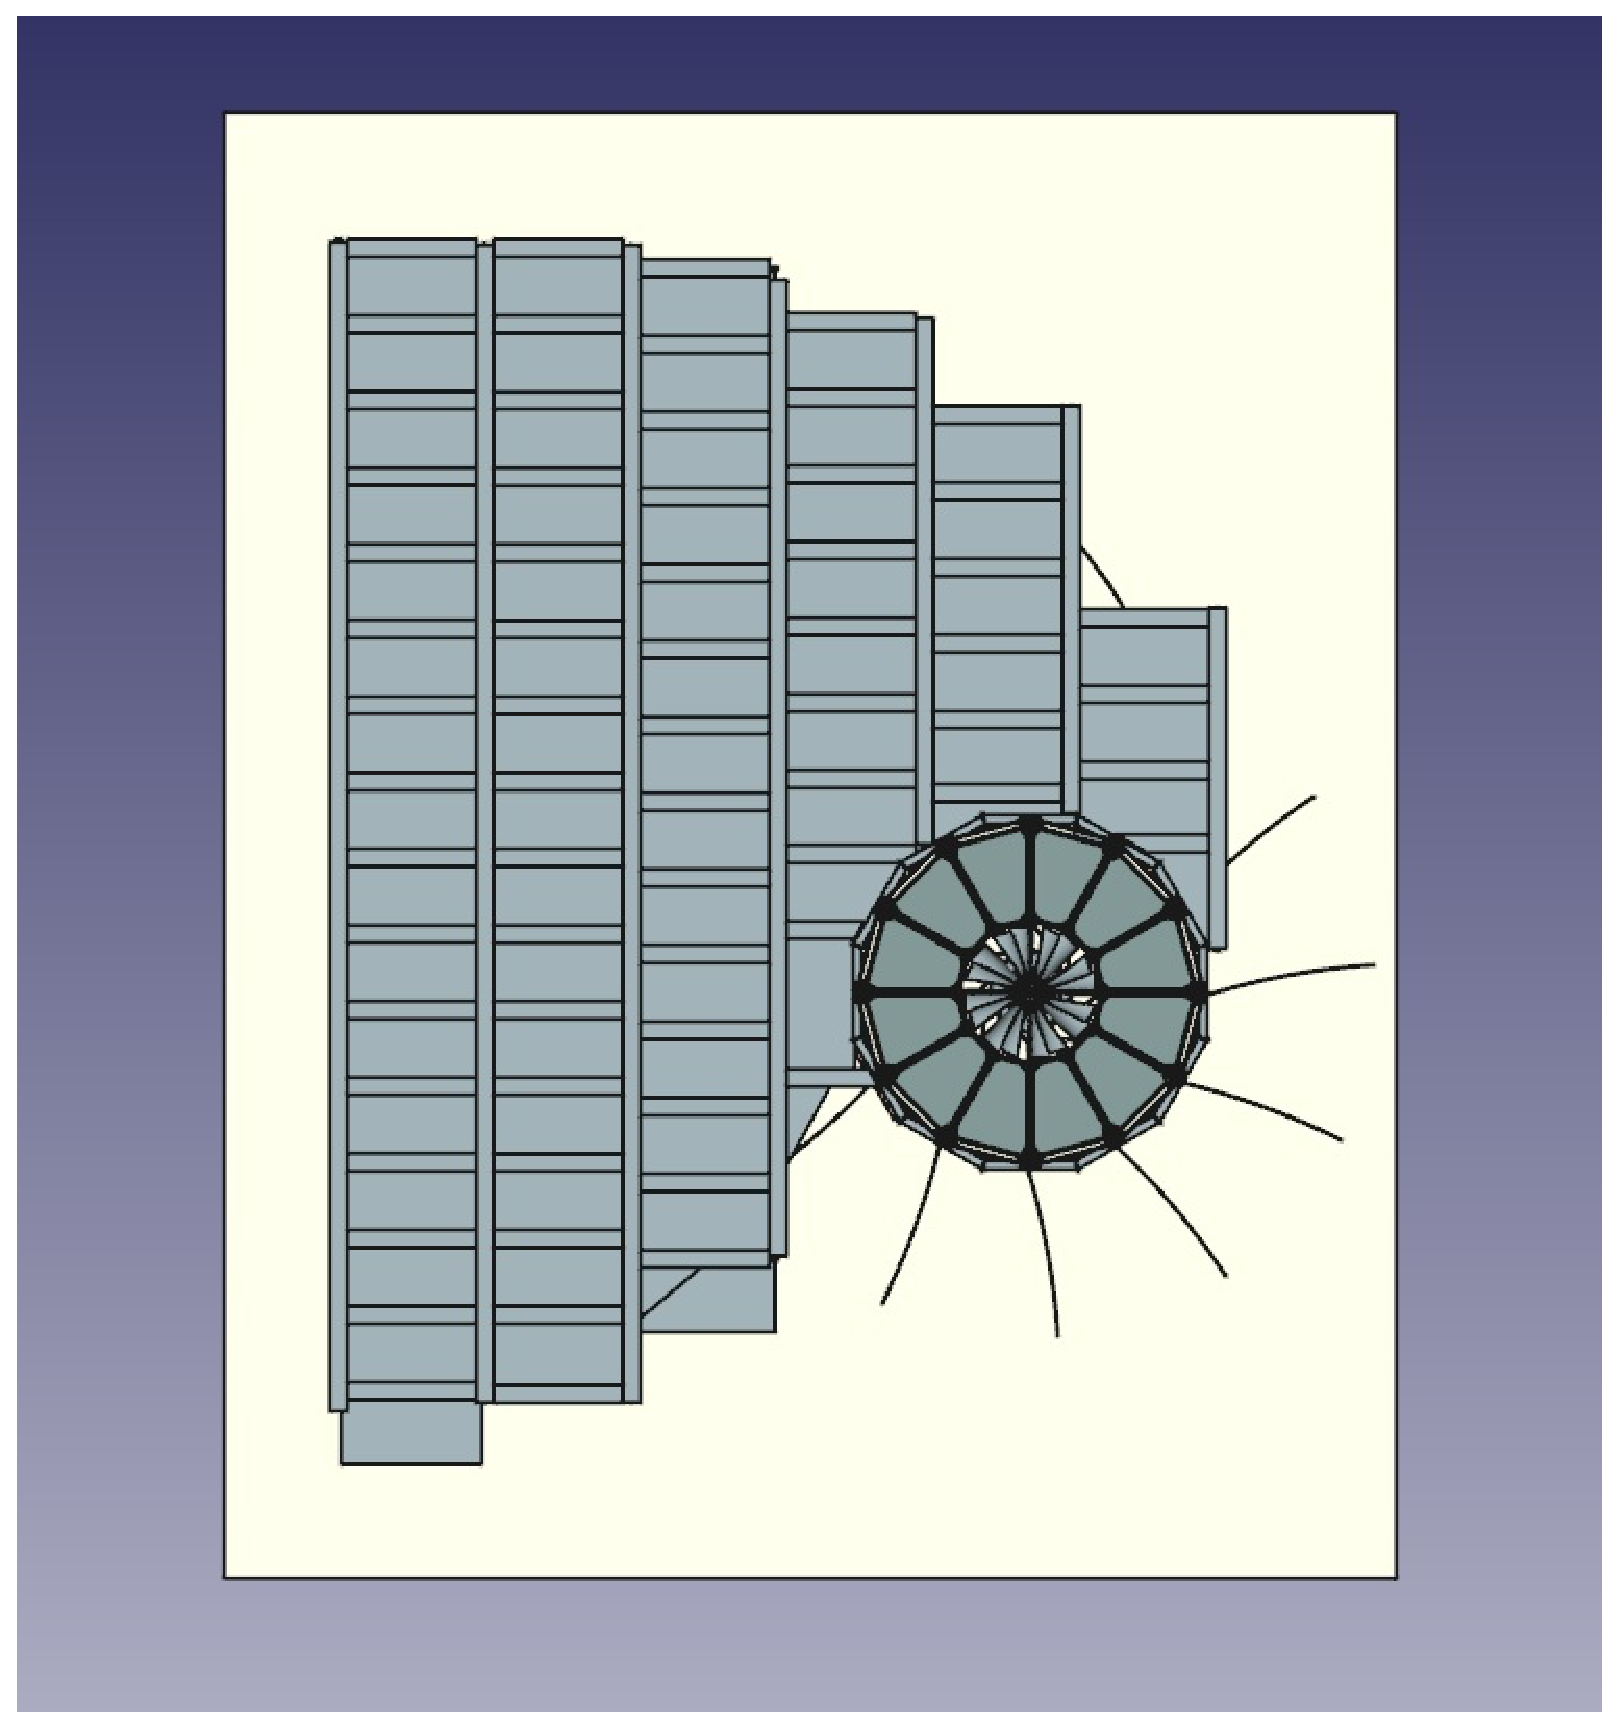
\includegraphics[width =0.7\textwidth]{figs/top_down_cad}
   \caption{A top view of the CAD drawing. The ``horizontal partitions''
   (designed to constrain the flow from leaving vertically) are clearly
   visible. In addition, the cone and turbine are also
   identifiable. Finally, the bottom tier vanes (which possess no
   horizontal partition) can be seen extending out the back of the
   device.} 
   \label{fig:top_down_cad}
  \end{center}
 \end{figure}

\begin{figure}[!htb]
  \begin{center}
   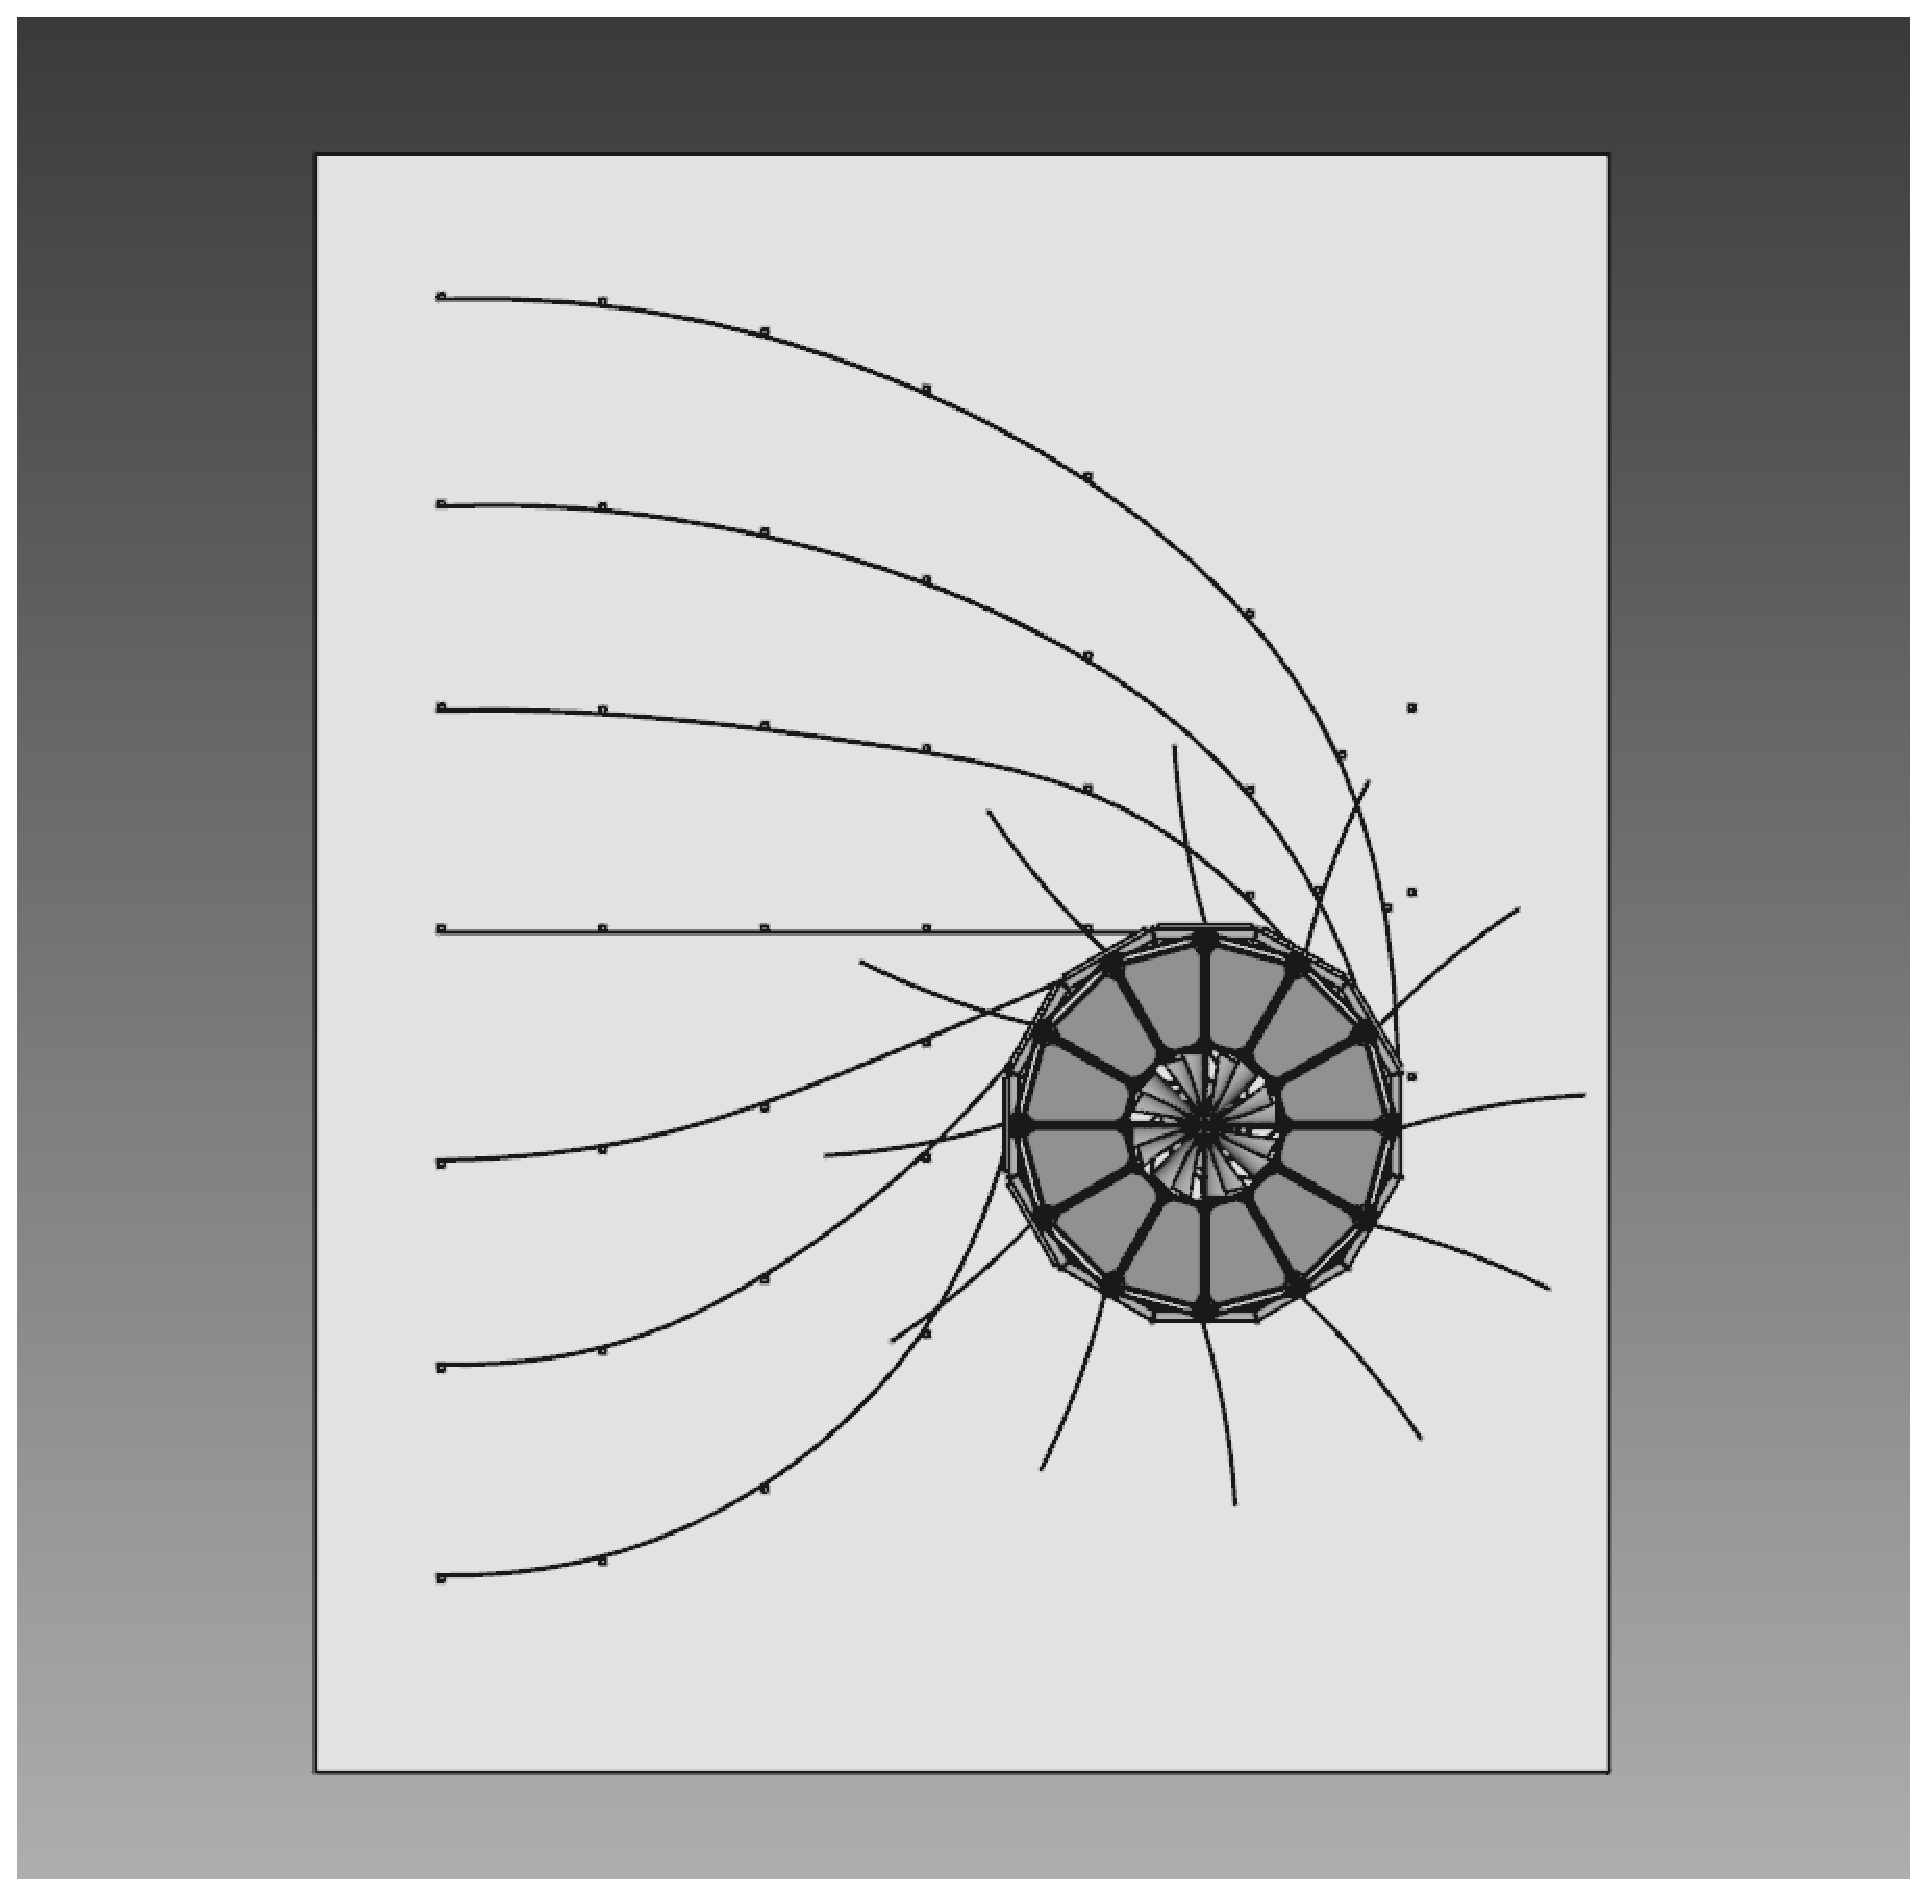
\includegraphics[width =0.7\textwidth]{figs/top_down_cad_notop}
   \caption{A top view of the CAD drawing, as in
   Figure~\ref{fig:top_down_cad}, but with the horizontal partitions
   removed. This provides a perspective on the second tier vanes, which
   extend out and in front (relative to the streamwise velocity) of the
   SoV.}
   \label{fig:top_down_cad_notop}
  \end{center}
 \end{figure}

\begin{figure}[!htb]
  \begin{center}
   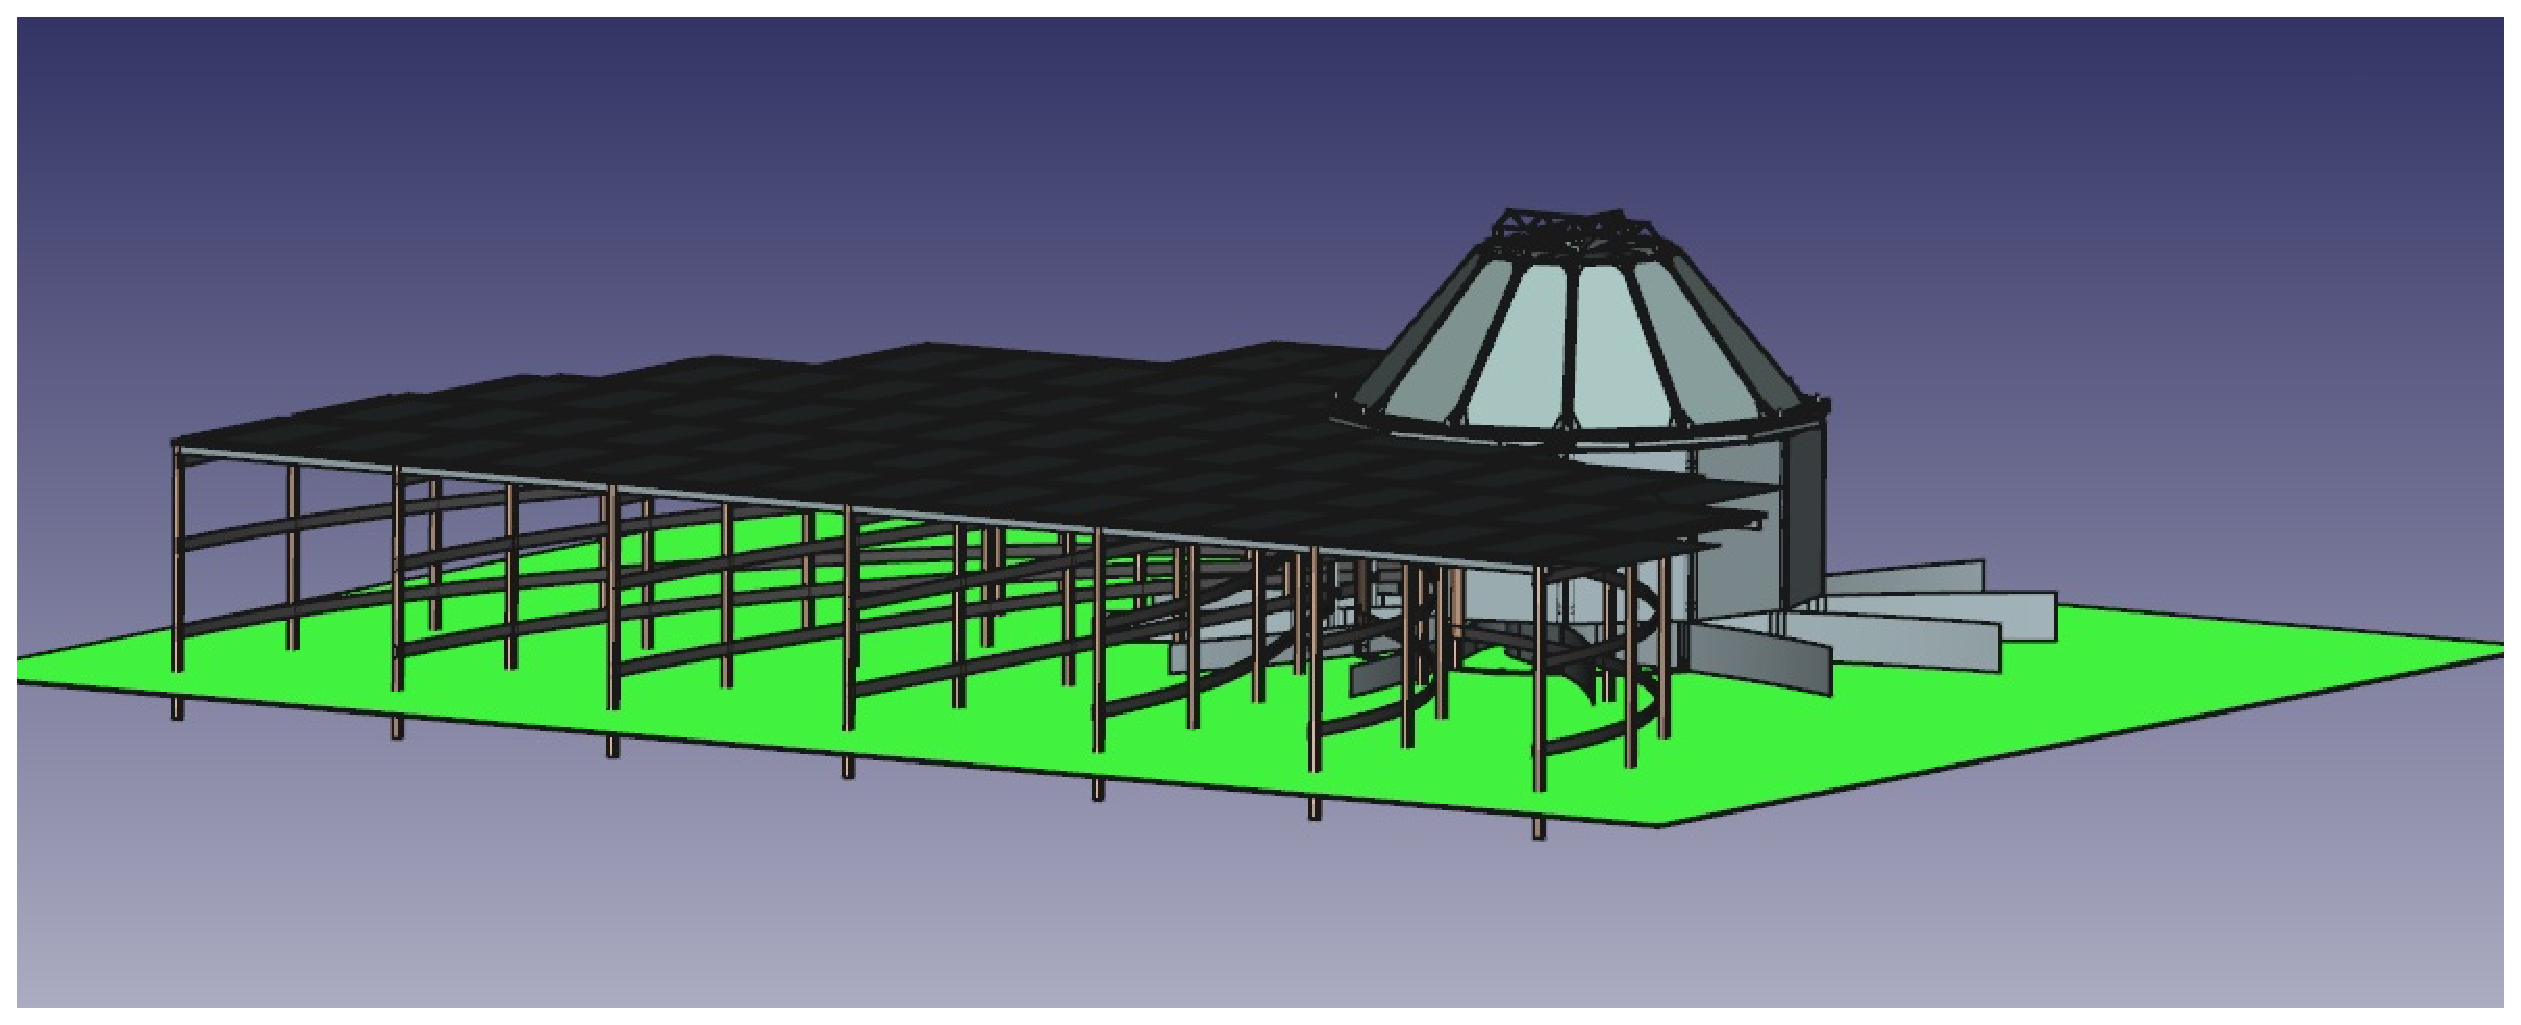
\includegraphics[width =0.7\textwidth]{figs/skewed_cad}
   \caption{A skewed view of the CAD drawings, which provides
   perspective on the height of the cone, the first and second tiers of 
   turning vanes, and the horizontal partitions.}
   \label{fig:cad_skewed}
  \end{center}
 \end{figure}

\subsection{Turning Vane Interpolation Functions}
\label{sec:interpolate}

The top tier design is now highly asymmetric, with a
large opening facing the incoming wind to capture incoming free stream
kinetic energy over a large area. The incoming flow enters the central
cylindrical area, where it spins and is driven out the top through the
cone. To enable these more asymmetric vane geometries for the top tier,
it was necessary to formulate a more general parameterization of the
vanes.

Previously, the vanes had a linear curvature function and were
axisymmetric. The new concept required the vanes to hold an azimuthal
dependence so that they are aligned with the streamwise velocity upstream 
of the device, and then curve inward to spin the flow at the center of
the device. A linear vane curvature was first attempted, but this was
found to have too few degrees of freedom to provide adjustments to the
vane curvature. Next, vanes that had an elliptic curvature were decided
upon. The intent here is to have a quarter of an ellipse, where the arc
of the ellipse starts at the x-intercept (thus ensuring the vane is
aligned with the freestream velocity) and then curves in towards the
center of the device, terminating at a high angle nearly azimuthal. To
accomplish this, the normal vector of the ellipse must be known. 

This required use of implicit differentiation for the functional,

\begin{eqnarray}
 f(x,y)  =& \frac{(x-h)^2}{a^2} + \frac{(y-k)^2}{b^2} = 1, \\
 \nabla f(x,y) =& \frac{2 (x-h)}{a^2} + \frac{2 (y-k)}{b^2}\frac{dy}{dx} = 0, \\
 \frac{dy}{dx} =& -\frac{(x-h)}{(y-k)}\frac{b^2}{a^2}. 
\end{eqnarray}
Where h and k are the elliptic intercepts and a and b are the
eccentricity of the ellipse along each axis. The tangent vector along
the ellipse is then,  
\begin{eqnarray}
 %{\bf \hat t} = {\bf e_x} + \frac{dy}{dx}{\bf e_y}, \\
 {\bf t} =& {\bf e_x} + \frac{dy}{dx}{\bf e_y}, \\
 {\bf t} =& \underbrace{\frac{(y-k)}{b^2}}_{a_y} {\bf e_x} -
  \underbrace{\frac{(x-h)}{a^2}}_{a_x}{\bf e_y} \\
 {\bf t} =& {a_y} {\bf e_x} - {a_x}{\bf e_y}. 
\end{eqnarray}

Noting that the normal vector has the form, 
\begin{eqnarray}
 {\bf n} =& {a_x} {\bf e_x} + {a_y}{\bf e_y}, \label{eqn:a_x}\\
 {\bf n} =& \frac{(x-h)}{a^2} {\bf e_x} + \frac{(y-k)}{b^2} {\bf e_y}.
\end{eqnarray}

This now defines the normal vector. However, we need to determine the 
constants (namely, $k,b$) that define ellipses that capture the shape we
desire. We want to determine an ellipse that has a certain
slope, m, at a specific point,  $(x_0,y_o)$, which lies on the inner
radius (R) of the SoV apparatus. This is shown in
Figure~\ref{fig:elliptic_vane_concept}. We have a system of four
equations,
\begin{eqnarray}
 \frac{(x-h)^2}{a^2} + \frac{(y-k)^2}{b^2} =& 1, \label{eq:ell1}\\
 \frac{(x_0-h)^2}{a^2} + \frac{(y_0-k)^2}{b^2} =& 1, \label{eq:ell2}  \\
 x_0^2 + y_0^2 =& R, \label{eq:ell3} \\
 -\frac{b^2}{a^2}\frac{(x_0-h)}{(y_0-k)} =& m. \label{eq:ell4} 
\end{eqnarray}
These equations express the fact that the ellipse intercepts both known
points, that the point $(x_0,y_o)$ lies on the inner radius of the
apparatus, and that the slope at this point is known. Assuming that
h, a, x, y, R and m are given, we have a system of four equations
(Equations \ref{eq:ell1}-\ref{eq:ell4}) with four unknowns,
$x_0,y_0,k,b$. This is, in principle, sufficient information to solve
this system. However, in practice, significant difficulties were
encountered. Inverting this system by hand is too complex and error
prone, and furthermore, Mathematica was unable to find a closed-form
solution. Numerous simplifications and additional constraints were added
to ensure that the system of equations were well-posed (a>b, for
instance), but the problem still resisted solution. 

 \begin{figure}[!htb]
  \begin{center}
   \includegraphics[width =0.95\textwidth]{figs/elliptic_vane_concept}
   \caption{The geometric problem for the elliptic vanes.}
   \label{fig:elliptic_vane_concept}
  \end{center}
 \end{figure}

The problem then, is that for a given location $(x,y)$ in space we are
unable to invert to determine the character of the ellipse that
intersects that point. Instead, we can pose the problem as discretizing
the arc along the inner radius of the vanes, we can generate data from
several curves that can be used to calibrate a 2D polynomial that will
smoothly vary in space. To accomplish this, we choose a series of
$x_0,y_0$ curves. For each unique ellipse defined by ($x_0,y_0,b,a,k$),
discretize at a uniform interval between $\left[-h,x_0\right]$, and
solve for the accompanying y-value, 
\begin{equation}
 y = -b \sqrt{1-\frac{(x-h)}{a^2}} + k. 
\end{equation}
One now has sufficient information to solve for the normal coefficients
$a_x$ and $a_y$ as defined in Equation~\ref{eqn:a_x}. This array of
coefficients specified at (x,y) are now fit to a 2D N\textsuperscript{th}
order polynomial. This has the form, 

\begin{equation}
 P(x,y) = \sum_{i=0}^N  \sum_{j=0}^N a_{i,j} x^i y^j
\end{equation}

where $a_{i,j}$ are coefficients of the polynomial which are selected by
minimizing the residual between the specified vane values and the
polynomial evaluated at that point. In other words, we find the
least-squares solution to a linear matrix equation, which is
under-determined. The solution to the equation $A x = b$ is found by
computing a vector $x$ that minimizes the Euclidean 2-norm $|| b - A x
||^2$. The polynomials were computed in separate python routines and
resulted in a generated input file. This specifies the vane angle
function within the region of the vanes. This function is then used as
part of the input for the field runs (see Appendix~\ref{sec:archiving}
for more details on the input file environment). 
%
% http://docs.scipy.org/doc/numpy-1.10.0/reference/generated/numpy.linalg.lstsq.html
%

 % \begin{figure}[!htb]
 %  \begin{center}
 %   \includegraphics[width = 15 cm]{figs/bottom_interp}
 %   \caption{Top view of the interpolation function for the ``right
 %   side'' of the vanes on the top tier. The red lines are the data sets
 %   that provides the input data used to calibrate the two dimensional
 %   polynomial field. The black line is the inner radius of the SoV.}
 %   \label{fig:bottom_interp}
 %  \end{center}
 % \end{figure}

The polynomial order was selected to be 7\textsuperscript{th} because it
provided a good balance between accuracy and a desire to maintain as low
an order as possible. Furthermore, the vanes interpolation was split
into two components, for the ``left'' and ``right'' (from the perspective of a
person standing upwind of the SoV and looking at it) of the vanes in the
top tier. This was found to be the most effective way to ensure that the
polynomial remained accurate without requiring very high order
polynomials. The accuracy of the interpolated field was checked by
``drawing'' vanes by seeding a particle upstream of the field and then
manually integrating it through the field using the scipy integrate ode
packages and verifying visually that the vane had the correct
character. Figures~\ref{fig:top_design} and~\ref{fig:bottom_design} were
generated using this technique. 
% The ``right'' interpolated field is shown in
% Figure~\ref{fig:bottom_interp}.\todo{update python plots} 

%
% /h2/nick/src/code/python/poly_vanes
%

\section{Turbine Design}
\label{sec:turb_design}

In addition to the final vane design, a turbine design was developed and
tested over a range of design conditions. The design parameters defining
the turbine are listed in Table~\ref{tab:turbine}. The exploration of the
turbine design space was conducted in a manner similar to the
optimization outline detailed in Figure~\ref{fig:opt_image}. The major
design improvements are detailed in Figure~\ref{fig:ut_turbine}. The
``initial guess'' was crude, with flat plate drag polars and a poor
initial guess for the blade angle of $\approx 10^{\circ}$. Later
designs use a higher blade angle often exceeding $40^{\circ}$. 
The design parameters that lead to the largest improvements in power
extracted were changes to the turbine blade geometry (from flat plate to
$180^{\circ}$ half cylinders to $90^{\circ}$ semicircles), optimization
of the blade angle and optimization of the turbine rotation rate. 
However, several other interesting improvements were found in addition to the
principle improvements, and are detailed below. 

  \begin{figure}[!htb]
   \begin{center}
    \includegraphics[width = 10 cm]{figs/turbine_opt}
    \caption{Initial turbine optimization before the coupling with the
    frozen flow. The ``initial guess'' was conducted with flat plate
    drag polars at a low blade angle ($\approx
    10^{\circ}$). Subsequent design improvements substantially improved  
    the power extracted, but this list constitutes only a ``greatest
    hits'' and the actual design improvements were highly iterative,
    with numerous runs of a particular parameter configuration yielding
    inferior power output. }
    \label{fig:ut_turbine}
   \end{center}
  \end{figure}

A gap in the center of the turbine was found to favorably reduce turbine
solidity and improve energy extraction. In some cases, this gap was
found to correspond to a mild downward flow as observed in the
fully-developed thermal-only cases detailed in
Section~\ref{sec:thermal_only}. The present simulations do not form a
two-celled vortex, but a gap in the center of the turbine is still
favorable. Similarly, while individual blades are not explicitly
represented in an actuator-disk model, the area of blades is a design
parameter and can be optimized. This is in essence a solidity or
blockage term, with more blades providing more surface area to extract
power from the fluid while simultaneously impeding the flow. A balance
between too much (a blocked off flow) and too little (too little blade
area to extract flow power) must be attained through optimization of the
controlling parameter, $mC$, the product of the number of blades and
each blade's chord length, as detailed in
Section~\label{sec:actuator_disk}. 

Improvements to the turbine power extracted were also attained by adding
``twist''. In other words, the blade angle varies as a function of
radius, i.e. $\beta = \beta(r)$. Our expectation is that the turbine
blades are inside the core vortex. Following our expectation of the
vortex velocity roughly following a Rankene profile, the angular
velocity in the inner core region follows a solid body rotation, 
\begin{equation}
 V_{\theta} = \Omega r . 
\end{equation}
As the torque imposed on the rotor also increases with radius, angular
velocity is increasingly more desirable to extract at larger radius, and
vertical velocity more desirable at smaller radius. Thus, our turbine
blade angle also changes linearly as a function of radius, with
a higher angle at larger radius. 

%Finally, cone improvement
After this initial exploration of the turbine design space, further
investigations were conducted in collaboration with Duane McCormick at
UTRC. This design was arrived at by comparisons between a ``frozen
flow'' optimization routine from UTRC  with the ``fully coupled'' CFD
described previously. This frozen 
flow Matlab code also used an actuator disk model as described in 
Section\ref{sec:actuator_disk}, and required the velocity profiles
immediately upstream of the actuator disk location from runs conducted
with and without the actuator disk present. Thus, the frozen flow
UTRC code was incapable of estimating the impact of a turbine on the
flow, and typically required updated velocity fields from the fully
coupled runs after several iterations. 
The UTRC code was not directly connected to the UT CFD code. Rather,
human intervention was required to prepare the velocity field outputs
from the UT CFD effort so that they could be used in the UTRC
code. Thus, the UTRC code would iterate through design parameters, and
then the CFD code was used as a higher fidelity confirmation. The UTRC
frozen flow optimization was largely consistent with the fully coupled
CFD prediction (see  Figure~\ref{fig:UTRC_turbine}, below). This has
resulted in two final rotor designs, with and without twist. This was
because the experimental team was not certain that a twisted design
would be feasible. Regardless, the twisted rotor was always predicted to 
out-perform the zero-twist rotor.  
The peak power extracted is predicted to be 2.14 kW for the rotor
with twist, and slightly more than 1.51 kW for a rotor with no twist. 
All of these results were conducted with the $90^{\circ}$ circular-arc
airfoil, as shown in Figure~\ref{fig:90_drag}. The load on the turbine
is predicted to be modest, at 20 ft-lbs. This indicates that the twisted
rotor design is extracting 44\% of the power from the flow, or a
Betz-efficiency of 75\%, which is consistent with the measured
efficiency of modern wind turbines. 
% after duane

  \begin{figure}[!htb]
   \begin{center}
    \includegraphics[width=.8\linewidth]{figs/utrc_plot}
    \caption{The power extracted by the rotor predicted by the CFD
    (dashed line) and frozen flow (solid line) for a range of rotor
    collective angles. The higher lines (red circles) are for blades
    with twist, and the lower (blue diamonds) are for constant blade
    angle runs, which was always  inferior in terms of power
    extracted. In general the frozen flow closely tracks the CFD.}
    \label{fig:UTRC_turbine}
   \end{center}
  \end{figure}

The proposed turbine design is shown in Table~\ref{tab:turbine}. Note
that the design parameter $mC $ is actually the number of blades
multiplied by the chord length. As detailed in
Section~\ref{sec:actuator_disk}, this is the actual parameter of
interest in the actuator disk formulation. For fabrication, this was 
decided to correspond to eight blades with a chord length of 0.45 meters
each. %\todo{discuss twist}  

\begin{table}[]
\centering
 \caption{The parameters for the optimized turbine design.}
\begin{tabular}{l|l|l|l}
Name                & Current Value    & Symbol           & Comments \\
 \hline
Outer Blade Angle & $70^{\circ}$ & $\beta_{\text{outer}}$  & linear twist between \\
Inner Blade Angle & $47^{\circ}$ & $\beta_\text{inner}$    & 
	     $\beta_\text{inner},\beta_\text{outer}$ \\ 
Chord Length * \# blades   & 3.6 meters  & $mC $ &  \\
Turbine rotation rate & 4.0 rad/sec  & $\omega$         &  \\
Blade Outer Radius  & 1.5 meters   & $B_\text{outer}$ &  \\
Blade Inner Radius  & 0.3 meters   & $B_\text{inner}$ &  \\
Height of turbine   & 4.5 meters   & $H_B$            & Height of turbine \\
\hline
\end{tabular}
 \label{tab:turbine}
\end{table}

As mentioned previously, the frozen flow and fully coupled CFD
agree. However this is only for rotor loadings close to those in the
coupled CFD. Substantial errors tended to appear in the frozen flow
predictions with parameters far from the coupled CFD. In some cases, the
limitations of the frozen flow optimization were significant. For
instance, the frozen flow model would consistently predict larger power
output at higher RPM. However, several attempts to extract more power at
larger RPMs would cause a breakdown of SoV flow in the coupled CFD
model, which resulted in the flow power dropping by more than an order
of magnitude.%\todo{add turbine flow pictures} 

  \begin{figure}
   \centering
   \includegraphics[width =0.45\textwidth]{figs/rotor_assem_oblique_1}
   \hfill
   \includegraphics[width =0.45\textwidth]{figs/rotor_assem_oblique_2}
   \\
   \vspace{1em}
   \includegraphics[width =0.45\textwidth]{figs/rotor_assem_side_render}
   \hfill
   \includegraphics[width =0.45\textwidth]{figs/rotor_assem_top}
   \\   
   \caption{CAD design images of the turbine. The CAD designs were
   created by the team at Georgia Tech based on the design
   specifications from the CFD performed by the author. The images were
   created from these CAD files by the author using
   FreeCAD\cite{Falck}.}  
   \label{fig:cad_turbine}
  \end{figure}


  \begin{figure}
   \centering
   \includegraphics[width =0.45\textwidth]{figs/turbine_built}
   \caption{The fabricated turbine. The cone superstructure is also
   visible.} 
   \label{fig:turbine_built}
  \end{figure}

%Shortcomings -- \todo{finish me}
%Designed for axisymmetric flow. 
%No wake correction as depicted in Section~\ref{subsec:wake_loss_model}.    

\section{Scenario Parameters}
\label{subsec:scenario_param}

With the system geometry defined, we need only impose the boundary
conditions defined in Section~\label{sec:bc} to have defined our
scenario of interest. However, as with the validation case shown in
Section~\ref{sec:field_val}, significant uncertainty exists in the
scenario parameters that define the ambient thermal and wind
conditions. Some discussion on the scenario parameters is therefore
warranted. 

The thermal boundary layer gradient was set based on data gathered by 
the Georgia Tech team in Arizona on June 9th, 2014. The raw data
presented in Figure~\ref{fig:thermal_profile_fit} is the average from
four vertical temperature profiles take at different times during a
single day. The measurements were gathered between 9:49 am and 1:43
pm\cite{ann_comm}.  

A particular challenge is that the closest measurement was taken by a 
thermocouple 1 mm above the pavement. Thus, the surface temperature and
magnitude of thermal gradient were not directly measured. To estimate
$T_0$ and $\Delta T$, the thermal profile was fit with a least squares
minimization of the residual between Equation~\ref{eq:bl_t} and to the
existing experimental data. The resulting profile is plotted in
Figure~\ref{fig:thermal_profile_fit}. The sparsity of existing
experimental data near the surface is quite clear from this
profile. The fitted profile is then evaluated at $x=0$ to determine the
ground temperature. Based on this criterion, a difference of 30 Kelvin was
selected.   

 \begin{figure}[!htb]
  \begin{center}
   \includegraphics[width = 15 cm]{figs/fit_zoomed}
   \caption{The raw thermal boundary layer data (blue circles) plotted
   against the fitted boundary layer profile (red triangles). The
   paucity of experimental data undermines the fit's accuracy to
   anything more than a plausible location for the actual wall
   temperature. }  
   \label{fig:thermal_profile_fit}
  \end{center}
 \end{figure}

In addition to the thermal profile, the incoming wind velocity needed an 
estimate. Thankfully, wind measurements were performed by the
experimental team in the field also during the June, 2014 test. A single 
hour time series was captured for both day and night as measured by the
sonic anemometers. These data series are plotted in
Figure~\ref{fig:wind_speed_estimate}. The wind speed was sampled at a
sampling rate of 0.5 Hz, and the traces were plotted for one hour (for
both the day and night). 

 \begin{figure}[!htb]
  \begin{center}
   \includegraphics[width=.7\linewidth]{figs/wind_measurements}
   \caption{Wind Speed Measurements from the June 2014 field test.}
   \label{fig:wind_speed_estimate}
  \end{center}
 \end{figure}

Several observations can be made from this data. There is essentially no
mean flow at night, but during the day the winds are not insignificant,
with a mean velocity of about two meters per second and fluctuations of
nearly six meters per second. It is clear that the wind profile is
turbulent.  Also note that the daytime wind does not die out: the
average horizontal velocity during the day is about 2-3 m/sec. 

The wind direction was also monitored, and showed little variation. 
This is shown in Figure~\ref{fig:wind_direction}. It was therefore
assumed that the wind had a constant heading and constant speed during
the simulations. Furthermore, discussions with the field team indicated
that wind heading over several years of field tests were relatively
consistent. This was part of the motivation for the movement to an
asymmetric vane configuration, as if the wind direction changed daily
(for instance) it would render an asymmetric design useless, unless it
could easily be manipulated to align with the free stream velocity. 

 \begin{figure}[!htb]
  \begin{center}
   \includegraphics[width=.7\linewidth]{figs/wind_direction}
   \caption{Wind direction measurements from the June 2014 field test.}
   \label{fig:wind_direction}
  \end{center}
 \end{figure}


% monin obuhkov should deal with this, no?
%It may well be that even in the "thermal only" cases there could be
%significant, zero mean turbulence (perhaps like grid turbulence)
%contributing from the ambient surroundings. 

\section{Solution Structure of the Field Configuration}
\label{subsec:field_predict}

\begin{figure}[!htb]
  \centering
  \includegraphics[width=.47\linewidth]{figs/u_field_vert}
  \hfill
  \includegraphics[width=.47\linewidth]{figs/w_field_vert}
  \\
  \includegraphics[width=.47\linewidth]{figs/T_field_vert}
  \hfill
  \includegraphics[width=.47\linewidth]{figs/v_field_vert}
  \label{fig:field_vert}
 \caption{Vertical slices through the middle of the vanes for the
 2016 Field Test. The top left is the streamwise velocity component
 (u), and the top right the vertical velocity, w. The bottom row shows
 the same plane, but now for the temperature field and azimuthal
 velocity. The turbine region is depicted at the top of the vanes as a
 white disk region.} 
\end{figure}

\begin{figure}[!htb]
  \centering
  \includegraphics[width=.45\linewidth]{figs/u_field_hor}
  \hfill
  \includegraphics[width=.45\linewidth]{figs/w_field_hor}
  \\
  \includegraphics[width=.45\linewidth]{figs/T_field_hor}
  \hfill
  \includegraphics[width=.45\linewidth]{figs/w_field_hor}
  \label{fig:field_hor}
 \caption{Horizontal slices through the top of the vanes for the
 2016 Field Test. The top left is the streamwise velocity component
 (u), and the top right the vertical velocity, w. The bottom row shows
 the same plane, but now for the temperature field and azimuthal velocity.} 
\end{figure}

The velocity and temperature fields resulting from the 2016 field test 
simulations are shown in Figures~\ref{fig:field_hor} and
~\ref{fig:field_vert}, below. Generally speaking, the fields have
complicated, non-trivial structure. The majority of the flow is driven
into the vanes by the ambient upstream winds, where it accelerates due
to the contraction of the vanes towards the center of the SoV.
The vertical slices in Figure~\ref{fig:field_vert} clearly depict a
strong vertical velocity in the center of the device. This vertical
plume coincides with a coherent, high temperature ``thermal plume'', as
well as a region of intense rotation and azimuthal velocity. This flow
is driven upward where it flows past the turbine and out of the top of
the device. 

From the horizontal viewpoint shown in Figure~\ref{fig:field_hor}, it is
clear that the streamwise velocity has a complicated structure. The
vertical velocity is largely a circular plume that has expanded to fill
the cylindrical inner region of the turbine vanes. Unlike in the
thermal-only cases, no downward flow exists, and there is no formation
of a two-celled vortex. 

\begin{figure}
  \centering
  \includegraphics[width=.7\linewidth]{figs/field_streamlines}
  \label{fig:field_stream}
 \caption{Fluid entrainment through and around the apparatus. This was
 drawn by seeding particles into the flowfield and then advancing them  
 using an RK4 time integrator. An outline of the inner enclosure region 
 is shown to provide a sense of scale. The bottom left corner is the
 upwind direction. While a majority of the flow is coming from upstream
 of the device, a substantial portion of the flow is nevertheless
 entrained from the leeward side of the SoV. }  
\end{figure}

Figure~\ref{fig:field_stream} shows tracing particles advanced forward
and backward in time from the center of the device. This clearly shows
that the flow is drawn in from both the front and back of the SoV, and
that the device is entraining air from a region far larger than the SoV
vane diameter.  While a majority of the flow is coming from upstream of
the device, a substantial portion of the flow is nevertheless  entrained
from the leeward side of the SoV. Most of the entrained flow from
downstream of the vanes comes from a narrower region than the upstream,
and appears to be constrained to the wake of the SoV. It is also
interesting to note that most of the backflow from downwind side occurs
very near the surface. While most of the radial inflow to the SoV is
from the downside side is near the surface, the vortex is strong enough
to entrain flow from outside the vanes above the device. 

The 2016 field configuration has 4.77 kW of kinetic energy flux through
the top of the vanes, taken from a plane just below the turbine, which
is 608\% more kinetic energy flux than the peak measurement produced in
the August 2015 Field test.  

\subsection{Sources of Error}
\label{sec:field_error}
%
%behaves like wind tunnel contraction
While these results are promising, there are several significant
shortcomings to these models and scenario conditions that substantially
impact the SoV performance. 

A major uncertainty is the opacity of the device. Ideally, the device
would be completely transparent. However, previous field tests
found that the SoV footprint resulted in shading in the inner region of
the vanes, which resulted in a lower temperature inside the device than
in the immediate region. As the physical trigger for the SoV is
initiated by thermal buoyancy, this necessarily greatly reduces the
velocities inside the device, and so the kinetic energy flux and power
extracted by the turbine. For instance, simulations performed where the
surface inside the region of the vanes was set to the ambient air
temperature (an admittedly ``worst-case scenario'') found that the
energy extracted by the turbine was reduced to only 800 Watts. Thus,
consistent with the results shown in Section~\ref{sec:wind_impact}, the
absence of a thermal to drive the flow reduces the available kinetic
energy flux (and thus, the power extracted by the turbine) by more than
half. 

%Scenario Uncertainty!!!!!!!!!!!

%Actuator disk under-estimates drag

%no model for drag on vanes (was reported by team)

%wind heading adjustments and measurements of flux reduction

No dynamics in the wind were considered, with only a steady,
non-zero mean wind velocity. It may well be that even in the "thermal
only" cases there could be significant, zero mean turbulence (perhaps
like grid turbulence) contributing from the ambient
surroundings. However, crude sensitivity analyses were performed by
adjusting the mean velocity of the wind by  $\pm 1 \text{m}/\text{s}$,
which indicated that the power generated by the turbine only increases
with higher wind velocity, and that most of the vortex structure and
character of the solution discussed in
Section~\ref{subsec:field_predict} remains true, with only modestly
reduced velocities. 

%It is also possible that a substantial transient may exist during which
%the SoV 

A June field test in 2016 reported only modest velocities through the
prototype apparatus.
While substantial, the uncertainties describe above are not significant
enough to account for the weakness of observed flow, indicating a
potentially significant model uncertainty that had previously not been
considered. The subsequent sections detail two possible modeling
inadequacy components that were investigated in detail, and may account
for the significantly reduced flow observed in the field. 

\section{Turning Vane Drag}

The first model correction proposed is to introduce drag along the
turning vanes to account for the skin friction along the surface. To
introduce a force of parasitic drag, the turning vane forcing 
representation described in Section~\ref{subsec:vane} need only be
modified to introduce an additional force that acts in opposition of the
fluid velocity. Thus, in addition to forcing the flow to align with the
vane surface, the flow will also be slowed. The vane formulation now
acts in a dissipative manner, and is not energy conserving. 

Our unit forcing vector $\hat f$ is simply the negative normalized inner
product of the velocity, $u$, and the turning vane tangent vector $\hat
t$,  
\begin{equation}
- \frac{u \cdot \hat t}{|| u \cdot \hat t ||} = \hat f. 
\end{equation}
The volumetric force applied is, 
\begin{equation}
 F = \hat f \, C_f \, \frac{1}{2} \frac{\rho || u ||^2}{\delta}
\end{equation}
Where $C_f$ is the skin friction coefficient (which must be determined),
$\rho $ is the density and $\delta$ the channel half width. 
For $C_f$, we use Dean's Correlation\cite{johnson1998handbook}, 

%ane
%
%https://books.google.com/books?id=JBTlucgGdegC&pg=SA13-PA51&lpg=SA13-PA51&dq=dean%27s+correlation+fluids&source=bl&ots=auW8XopUC9&sig=DDxuQONFvqly5KQOocSPr39rS70&hl=en&sa=X&ved=0ahUKEwii3vX9wZHOAhXmxYMKHUqlChYQ6AEIJTAB#v=onepage&q=dean%27s%20correlation%20fluids&f=false 
%
\begin{equation}
 C_f = 0.073 \, (Re)^{-0.25}. 
\end{equation}
Where the Reynolds number is defined as, 
\begin{equation}
 Re = \frac{u\, \delta}{\nu}.
\end{equation}

Some roughness elements exist across the vanes. In addition to
non-smooth surface materials, the design of the field test apparatus
ultimately relied upon posts to hold the turning vanes. These posts were
pieces of wood which were modeled as roughness elements. In order to
determine $C_f$ for these cases, the Colebrook formula\cite{Colebrook367},
% Colebrook, C. F.; White, C. M. (3 August 1937). "Experiments with
% Fluid Friction in Roughened Pipes". Proceedings of the Royal Society
% of London. Series A, Mathematical and Physical Sciences. 161 (906):
% 367–381. doi:10.1098/rspa.1937.0150 
was used to provide an estimate for the friction factor given a
roughness height, $\epsilon/D$,  
\begin{equation}
 \frac{1}{\sqrt{f}} = -2.0 \text{ log}\left(\frac{\epsilon/D}{3.7} + \frac{2.51}{Re\sqrt(f)}\right).
\end{equation}
 With the assumption that for large roughness the Reynolds number term
 contribution is not significant, the function is no longer implicit in
 $f$ and can be determined directly, 
\begin{equation}
 f = \left(2.0 \text{ log}\left(\frac{\epsilon/D}{3.7}\right)\right)^2. 
\end{equation}
%Then, a Moody chart was consulted to provide the the 
Note that D here is the hydraulic diameter which must account for the
two plates (we treat the vanes as a channel),
\begin{equation}
D_H = \frac{4 A}{P} = \frac{4 (2w)\delta}{2w} = 4 \delta
\end{equation}
Where $\delta$ is the channel half width, or in our case, the distance
between the vanes. To construct a ``worst-case'' scenario, we consider
the smallest distance between the vanes, which occurs near the center of
the SoV. Furthermore, we consider roughness heights based on a
two-by-four (which were used as supports for the
vanes). Even for this worst case scenario, the velocities on the vanes
are not substantially reduced with the addition of the drag model. The
flow field kinetic energy flux was never reduced more than 12\%. 
This crude model indicates that the reduced flows observed during the
June 2016 field tests are not attributable to skin friction drag on the
turning vanes.  


\subsection{Blade Solidity Modification}
\label{sec:solidity}
%
%https://en.wikipedia.org/wiki/Blade_solidity
%
It was noted that wind turbines typically possess three blades, versus
the eight blades used in the 2016 field test. This is therefore a
substantially increased turbine solidity versus common engineering
designs. It is expected that we are operating in a regime not common to
typical actuator disk models. 

The power output of a turbine is proportional to the thrust that it
exerts onto the flow, and the larger the thrust, the larger the flow
resistance the turbine presents to the flow. The maximum power for any
wind turbine must lie in between two extremes, i.e. high and
a low impedance both result in minimal power
extraction\cite{solidity_oxford}.  

For the case of high impedance, little fluid flows through the
turbine and instead flows around the device. This gives the appearance of
the turbine being ``blocked''. In the case of low impedance, the turbine
hardly affects the flow, and less power is extracted than could be. 

Thus, an ``efficient'' impedance to the flow is one that strikes the 
right balance between solidity and tip speed ratio. If the solidity is
high, the operating tip speed ratio must be lower to avoid too high an
impedance. 

However, it is hard to predict the precise effects of the various
phenomena, which is why it is difficult to comment on the overall
performance of a particular machine in a specific
scenario. %Turbine design is highly specialized for 

However, the actuator disk model treats the flow in the disk region as
if it was flowing through a rotor with identical solidity but an
infinite number of blades. A model correction was introduced that
attempts to represent the fact that as the number of turbine blades
increases, the pressure across the actuator disk should rise. This is
accomplished by adjusting the area of the actuator disk down by the
ratio of the free area in the disk versus the blade sizes. 

%A second model correction was therefore introduced with the aim of attempting to
%discern if the turbine 


% too high an impedance
%This has several important implications.  

%A low tip speed ratio implies increased torque, requiring a larger
%and higher cost gearbox. In addition, the lower the tip speed ratio, the
%higher the maximum angle of attack, which can be problematic with regard
%to blade stalling. 

%
% howevr, it is hard
%

%When applied to a rotor with a finite number of blades, 


The length of each blade blocking vertical flow in the actuator disk is, 
\begin{equation}
  Ch * \text{Cos}(\beta(r)) = Ch_x(r). 
\end{equation}
The total length in an annular region that is blocking is therefore,
\begin{equation}
  N * Ch_x(r) = l_B(r),
\end{equation}
Where N is the number of blades. 
Then, the ratio of an annular length that is impeded by blades is, 
\begin{eqnarray}
 B(r) =& \frac{2\pi r- l_B(r)}{2 \pi r}\\
 B(r) =& 1- \frac{l_B(r)}{2 \pi r}. 
\end{eqnarray}
Note that a ``floor'' function is needed to ensure the solidity ratio
does not go below zero. 

For a 1D control volume analysis for the region, the continuity
equation is, 
\begin{eqnarray}
 \rho V_z' A' =& \rho V_z A,\\
 V_z' =& V_z \frac{A}{A'}, \\
 V_z' =& \frac{V_z}{B(r)}.
\end{eqnarray}
This implies that $V_z' \rightarrow \infty$ as $A' \rightarrow
0$. This is as expected, as the blockage becomes more severe, the flow
would need to move at greater speed to go through it. 

The flow angle with respect to turbine velocity is therefore modified 
from Equation~\ref{eq:fan_direction} in
Section~\ref{sec:actuator_disk},
\begin{equation}
 \theta_f = \text{tan}^{-1}(\frac{U_{\text{up}}}{U_{\text{fwd}}})
\end{equation}
to,
\begin{equation}
 \theta_f = \text{tan}^{-1}(\frac{U_{\text{up}}}{B(r) U_{\text{fwd}}}). 
\end{equation}
As $B(r) \rightarrow 0$, $\theta_f \rightarrow \pi$, e.g. 90 degrees. In
this way the velocity vector will be completely aligned with drag. 

Furthermore Equation~\ref{eq:force_turb}, 
\begin{equation}
 F = \frac{1}{2}\frac{c \rho U_p^2}{A}(C_L \cdot n_{\text{lift}} + C_d
  \cdot n_{\text{drag}})
\end{equation}
is modified so that, 
\begin{equation}
 \bar U_p^{2} = \left(\frac{U_p}{B(r)}\right)^2
\end{equation}

This turbine modification for solidity has a significant impact on the
power extracted by the turbine. A comparison between the number of
turbine blades and the power generated by the turbine for both the
baseline turbine and the turbine with the solidity modification is shown in
Figure~\ref{fig:turbine_solidity}. The results are quite consistent with
two blades, show a notable inconsistency at four blades, and completely
diverge at higher blade count. 
%Only even number of blades were
%considered due to the expectation that 

  \begin{figure}[!htb]
   \begin{center}
    \includegraphics[width = 10 cm]{figs/solidity}
    \caption{The power extracted by the turbine as a function of blade
    count. The blue straight line indicates the turbine model as defined
    in Section~\ref{sec:actuator_disk}, and the red dashed line
    indicates the power output of the turbine after the solidity
    modification.}
    \label{fig:turbine_solidity}
   \end{center}
  \end{figure}

This model modification indicates that the prior prediction of eight
turbine blades in Section~\ref{sec:turb_design} was too large. Instead,
a turbine with substantially reduced solidity is preferred. Based on
Figure~\ref{fig:turbine_solidity}, a turbine with similar
characteristics in terms of length, location and twist but reduced from
eight blades to four or two blades is expected to mitigate the
substantially reduced performance observed in the field. 

This crude model is admittedly extreme, as it effectively models the
blades as flat plate bluff bodies, with the flow completely
separated on the leeward side. Ideally, the flow should be smoothly
turning through the blading, and not separate. Thus, it is possible that
this estimate is overly pessimistic. Regardless, this is the only model
correction that was explored that is plausibly capable of explaining the
2016 field observations noted in Section~\ref{sec:field_error}. 

Interesting enough, there have been actuator disk models used with wind
turbines that indicate operating at low tip speed ratios with high
solidity ratios would possess power coefficients close to Betz-like
limits of efficiency\cite{WE:WE118}. It is therefore possible that the
actuator disk model is generally unsuited for high solidity regimes, and
that the correction presented here is more generally useful. 

%todo\todo{what about shading?}

\section{Estimating the Upper Limit on Power Extraction}
\label{sec:peak_estimate}

All of the results in Section~\ref{subsec:field_predict} were generated
using $90^{\circ}$ semicircle blade geometries, as shown in Figure
\ref{fig:90_drag}. The only other blade geometries considered were the
flat plate and $180^{\circ}$ arcs, which were universally found to be
inferior. Time constraints required fabrication of the turbine in short
order, and a limited budget encouraged inexpensive (and therefore
simple) turbine blades. Finally, the design space was limited to
readily available drag polar data due to the expense and difficulty of 
fabricating non-standard turbine blades. Risk mitigation also played a
role, with an emphasis on traditional, and therefore well-vetted turbine
blade design. %While several comparisons have been performed with
%different choices of turbine blades (flat plate, 180 degree semicircles,
%etc. ) this was not an exhaustive survey. 
%Nevertheless, this is not an exhaustive exploration of turbine
%blade design, and the question remains, ``Could more power be extracted
%with a different rotor geometry?''. 
This section details an additional computational research program
performed after the turbine fabrication with the intent of estimating
the upper limit of power extraction with an idealized turbine. 

Practical utility-scale wind turbines achieve at peak 75\% to 80\% of
the Betz limit\cite{burton2001wind}. The Betz-limit states a theoretical
maximum of 59\% of the wind's power may be captured. Therefore,
practical wind turbines extract less than half of the available kinetic
energy flux. 
Comparing the kinetic energy flux of simulations without the turbine to
the power extracted by the turbine, we note that our simulations
typically predict power extraction ratios slightly less than fifty
percent, indicating that our efforts are not significantly better or
worse than could be expected. While this provides an estimate, the
Betz-limit is likely not accurate for this case. Any analysis of the
power that can be extracted is complicated by the presence of
considerable vertical and azimuthal flow in the vortex, and so the
design considerations are different from those for a classical wind
turbine.  

The objective then, is to formulate a more generalized approach to the
turbine vane parameters to permit an optimization that is not
constrained to a particular turbine blade geometry. Rather, this
approach seeks to estimate the upper limit of power extracted. The
rationale behind this is to provide an upper bound on the power that can 
be extracted for a particular configuration, which can then be used as
input for feasibility considerations of the SoV.  

It is desirable to perform these estimates within the context of the
actuator disk model (see Section~\ref{sec:actuator_disk}). While
actuator disk models are commonly
optimized\cite{790585,WE:WE487,en5093425,adkins1983design}, the lift and 
drag polars are not parameters that are varied in these schemes. Rather,
a given blade geometry is assumed and then the rotation rate, blade
angle and chord length (for instance) are optimized.   

Conversely, airfoil optimization is a rich field with sophisticated and
well-vetted
techniques~\cite{drela1998pros,lewis2001aerodynamic,Chehouri2015361},
but these methods do not use an actuator disk model, and focus on the
shape optimization of the airfoil geometry (and through this, the lift
and drag polars).  

To address the possibility of further turbine blade
improvements, while continuing to use an abstract actuator disk model,
%while simultaneously not representing the blade geometry
%proper
this section details a formulation for a generic set of drag 
polars. These generalized drag polars permit exploration of a broader
design space. The optimization of this model can be fully coupled to the
flow, and so does not violate any Betz-like considerations that might
similarly arise in an analysis of frozen flow fields.
The drag polars are selected to be generic functions and are optimized to
maximize the power extracted by the rotor. While the resulting drag
polars might not be physically  realizable, they represent a ``best
case'' upper bound indicating the peak power that might be extracted
with further rotor design iterations. This ``limiting case'' is useful
for evaluating the system feasibility from a technological standpoint,
by providing the peak power that could be extracted for a given vane
geometry. 

The power extracted by the turbine is, 
\begin{equation}
 P = \Omega \, Q
\end{equation}
where the torque, Q, is\cite{morgado2014validation}, 
\begin{equation}
 Q = A_R \int_0^{2\pi} \int_{r_{\text{min}}}^{r_{\text{max}}} F''_{\tau}\, r\, dr d\theta.
\end{equation}
Here, $A_R$ is the relative area coefficient which is, 
\begin{equation}
A_R = \frac{c B (r_{\text{max}}-r_{\text{min}})}{\pi(r_{\text{max}}^2-r_{\text{min}}^2)}
\end{equation}
where B is the number of blades, $r_{\text{max}}$ and $r_{\text{min}}$
are the turbine radii, and $F''_{\tau}$ is the force per unit
area on the turbine, which is, 
\begin{equation}
 F''_{\tau} = \frac{F_{\tau}}{cl}= \frac{1}{2}\rho U_R^2 \, C_{\tau}.
\end{equation}
with $U_R$ the magnitude of relative velocity and $c$ is the blade chord
length, which is assumed to be constant (not a function of the radius,
for instance). Finally, $C_{\tau}$ is the tangential force coefficient,
which depends on the local lift and drag coefficients, and the
flow angle, $\phi$, 
\begin{equation}
 C_{\tau} = C_L \,\text{sin}(\phi) + C_D \,\text{cos}(\phi)
\end{equation}
Combining the equations above results in an expression for the power
that explicitly depends on the lift and drag coefficients, 
\begin{equation*}
 P = \frac{\Omega \rho c B (r_{\text{max}}-r_{\text{min}})}{2 \pi(r_{\text{max}}^2-r_{\text{min}}^2)}
\int_0^{2\pi}
\int_{r_{\text{min}}}^{r_{\text{max}}} U_R(r,\theta,\Omega)^2 \left(C_L
						     \,\text{sin}(\phi)
						     + C_D
						     \,\text{cos}(\phi)
						    \right) r\,dr d\theta. 
\end{equation*}
We lump the constant terms together, 
\begin{equation}
E_{\tau} = \frac{\Omega \rho c B (r_{\text{max}}-r_{\text{min}})}{2
 \pi(r_{\text{max}}^2-r_{\text{min}}^2)}
\end{equation}
 and separate this equation, 
\begin{align}
 P_L = E_\tau
 \int_0^{2\pi}
  \int_{r_{\text{min}}}^{r_{\text{max}}} U_R(r,\theta,\Omega)^2 \, C_L(\phi,r)
 \,\text{sin}(\phi)\, r\,dr d\theta,  \label{lift} \\
 P_D = E_\tau
 \int_0^{2\pi}
  \int_{r_{\text{min}}}^{r_{\text{max}}} U_R(r,\theta,\Omega)^2 \, C_D(\phi,r) \,\text{cos}(\phi)\, r\,dr d\theta. \label{drag}
\end{align}
Note that we have assumed $C_D = C_D(\phi,r)$ and $C_L = C_L(\phi,r)$,
namely, that the coefficients vary with the flow direction and may vary
radially, due to twisting the blade angle. Furthermore, the flow
direction, $\phi$, varies with the location and the blade speed,
in that $\phi=\phi(r,\theta,\Omega)$. The relative velocity is the
quantity, $U_R = U - U_\tau$, e.g. the difference in velocity between
the turbine and the flow. The turbine has no axial velocity ($w_\tau =
0$) and a constant rotation speed, and so the two components of velocity
in the plane of rotation can be expressed as,
\begin{align}
 u_\tau = \Omega \,r\, \text{sin}(\theta)\\
 v_\tau = \Omega \,r\, \text{cos}(\theta)
\end{align}

Our objective is now to discover what these unknown functions of lift
and drag are. To do this, we specify an optimization problem such that, 
\begin{equation*} 
 \text{Max } P(C_L,C_D) \quad \text{ subject to: }
  \begin{cases}
   |C_L| < C_L^{\text{Max}}, \\
   0 < C_D < C_D^{\text{Max}}. \\
  \end{cases}
\end{equation*}

In words, the drag must be specified to be greater than zero, but
the lift can be negative. This is a problem in the calculus of
variations, where the objective is to maximize a
functional subject to imposed
constraints~\cite{thornton2004classical,bradbury1968theoretical,2015JFM...784..565S}.   

%
% does this argument still work?!?
%
The integral shown in Equation \ref{lift} above can be bounded by 
Schwarz's inequality,  
\begin{align*}
  \left[
    \int_0^{2\pi}
    \int_{r_{\text{min}}}^{r_{\text{max}}} C_L(\phi,r)\, U_R(r,\theta,\Omega)^2
 \,\text{sin}(\phi)\, r\,dr d\theta \right]^2 \le \\
  \int_0^{2\pi} \int_{r_{\text{min}}}^{r_{\text{max}}} C_L^2(\phi,r) dr d\theta\,
  \int_0^{2\pi} \int_{r_{\text{min}}}^{r_{\text{max}}} U_R(r,\theta,\Omega)^4 
 \,\text{sin}^2(\phi)\, r^2\,dr d\theta.
\end{align*}

In this way the first integral quantity,
\begin{equation}
  \int_0^{2\pi}
 \int_{r_{\text{min}}}^{r_{\text{max}}} C_L^2(\phi,r) dr d\theta, 
\end{equation}
is clearly maximized when $C_L(\phi,r) = C_L^{\text{max}}$. 
The result for Equation \ref{drag} is identical. Now, for these
conditions, we are interested in largest attainable values. For the drag
coefficient, $C_D^{\text{Max}}$ is two. % refmunson 
This corresponds to a flat plate perpendicular to the flow.
The lift coefficient peak is about 1.75. This design is not necessarily
physically realizable, but represents an absolute maximum. 

Therefore, our lift/drag functions may be expressed as,
\begin{align*} 
 C_D(\phi) = \bar C_D \, \psi(\phi) 
  \begin{cases}
   \psi(\phi) = 1 \text{ if sin}(\phi) > 0,   \\
   0 \text{ else} \\
  \end{cases} \\
 C_L(\phi) = \bar C_L \, \Psi(\phi) 
  \begin{cases}
   \Psi(\phi) = 1 \text{ if cos}(\phi) > 0,   \\
   -1 \text{ else}. \\
  \end{cases}
\end{align*}
Where $\bar C_L = 1.7$ and $\bar C_D = 2.0$. The plot of these drag
polars are shown in Figure \ref{drags}. 

\begin{figure}[!htb]
  \begin{center}
    \includegraphics[width = 12 cm]{figs/opt_drags}
    \caption{The uncalibrated idealized drag polars.} 
    \label{drags}
  \end{center}
\end{figure}

%Thus, the drag polars
%have the form, 
%\begin{align*} 
% &C_L(\phi) = 
%  \begin{cases}
%    1.75& \quad 0^{\circ} \le \phi \le 180^{\circ}, \\
%   -1.75& \quad 180^{\circ} \le \phi \le 360^{\circ}.  \\
%  \end{cases}\\
% &C_D(\phi) = 
%  \begin{cases}
%    2.0& \quad -90^{\circ} \le \phi \le 90^{\circ}, \\
%      0& \quad 90^{\circ} \le \phi \le 270^{\circ}.  \\
%  \end{cases}\\
%\end{align*}

Under this approach, the turbine extracts so much energy from the flow
that the vortex loses its coherence and the power extracted becomes
negative (e.g. the constant velocity turbine is adding energy to the
flow). %\todo{add image}
This implies a limit on how much of the energy can be extracted before
disrupting the flow so greatly that the vortex cannot be maintained.   
Consistent with the results from Section~\ref{sec:field_error},
the vortex is not robust, and the feedback from extracting more power
from it (manifest as increased blade solidity) causes a collapse of the
vortex structure. It is interesting to note that the vortex collapse is
not subtle, with the power extracted discontinuously dropping to zero or
negative values. 

To withdraw from the vortex disruption point, the drag
polars are calibrated by reducing $\bar C_L $ and $\bar C_D$ so that the 
vortex does not dissipate and the power extracted remains positive. The
parameters were adjusted by hand, so the calibration is crude. The
optimal parameters found were $\bar C_L = 1.1$ and $\bar C_D = 1.5$. It
is interesting to note that this is nearly the average of the drag
polars shown in Figures~\ref{fig:flat_plate_drag},~\ref{fig:semi_drag}, 
and\ref{fig:90_drag}. The solution flow in the case of the idealized
turbine remains similar to the results shown in
Section~\ref{subsec:field_predict}, and so are not depicted here. 

The steady state power extracted by the ideal turbine 
increased from the previous best attained with the 90 degree
semicircles, to 2.76 kW. It is interesting to note that this is 58\% of
the available kinetic energy flux measured just upstream of the turbine,
indicating that the turbine is very close to the Betz-limit of
59.3\%. While as indicated previously, the Betz-limit is likely to be
inaccurate for rotating flows, it is nevertheless interesting that the
idealized turbine would extract power so close to the maximum predicted by
Betz.  This provides a weak limit (even under these idealized
conditions) bounding the power that can be derived from this
flow. Furthermore, this indicates that previous estimates of the power
that might be extracted from the flow are not greatly limited by the
present turbine design. This is an important element of the system
feasibility assessment, as it provides evidence against the turbine
being a source of considerable inefficiency.  

%discredits any 

% as it implies that any assessments of the system feasibility 


\chapter{Characteristics of Synthetic Dust-Devils}
\label{sec:results}

%
% RESULTS TODO
%
% need to motivate optimization workflow and plans
% current ideas not bad, need more
%
%

The computer simulations in the proposed study are intended to discover
the optimal solar vortex system configuration for a range of scenarios
and system sizes. This section contains discussions of the preliminary
simulation results to motivate that the existing simulation capability
is sufficiently well developed and understood to permit an efficient
exploration of the SoV configuration space. 
This section begins with a discussion of the structure of solutions from
a representative case with no ambient winds, the ``thermal only''
scenario. Next, a case with strong ambient horizontal winds (``Wind'')
is discussed. Finally, the results from a series of runs are shown to
demonstrate a heuristic by which incremental optimization of the system
configuration will be conducted\todo{fix this sentence}.

%The results of these optimized configurations will be used as input
%for the design of a prototype to be tested in Mesa, Arizona this
%summer. 

% \todo{add photo}
  % \begin{figure}[!htb]
  %  \begin{center}
  %   \includegraphics[width = 12 cm]{figs/sov_field}
  %   \caption{A photo of the field configuration, during the June 2015
  %   Field Test.}
  %   \label{fig:field_real}
  %  \end{center}
  % \end{figure}

\section{Thermal Only}

While ambient winds in the field impact system performance, it is
also illuminating to consider an idealized scenario with natural convection
driven only by thermal instabilities. Simulations of this baseline,
thermal-only flow are intended to ensure the SoV apparatus to form a
strong thermal plume even in the absence of wind. 

In this section a representative case of an optimized thermal-only SoV
configuration is presented. This is a simple curved vane configuration with
two-tiers with ground temperature of 335 Kelvin and a freestream
temperature of 313 Kelvin. There is no ambient velocity and the boundary
conditions are as described in Chapter \ref{sec:bc}. 

The two tiers of vanes used for these cases are drawn in Figures
\ref{fig:thermal_vane_bottom} and \ref{fig:thermal_vane_top}.
 Note that in the
configuration, the vanes are 
aligned radially at the largest radius, and then increasingly curve
towards azimuthal at smaller radius. Note that these are representative
curves of the body forcing field, and do not actually represent vane
surfaces. The vanes are represented as in Chapter \ref{subsec:vane}. 
These images are created by tracing the path a particle follows through
the forcing field. The region of forcing is between $\{0.3-0.9\}$ meters
for the bottom tier, and $\{0.6-0.9\}$ meters for the top tier. Overall,
the system is 1.1 meters tall, with the short first tier only standing
0.132 meters high. The top and bottom tiers have final angles of
$70^{\circ}$ and $85^{\circ}$, respectively. No cone is used in this
case. 

\begin{figure}[htb]
\centering
\begin{minipage}{0.45\textwidth}
\centering
 \includegraphics[width=.8\linewidth]{figs/bottom_thermal_only}
 \caption{Horizontal drawings of the curvature functions for the bottom tier
 vanes. The max angle is $85^{\circ}$, or $5^{\circ}$ less than azimuthal.}
 \label{fig:thermal_vane_bottom}  
\end{minipage}\hfill
\begin{minipage}{0.45\textwidth}
\centering
\includegraphics[width =0.8\textwidth]{figs/top_thermal_only}
\caption{Horizontal drawings of the curvature functions for the top tier
 vanes. The max angle is $70^{\circ}$, or $20^{\circ}$ less than
 azimuthal.} 
 \label{fig:thermal_vane_top}  
\end{minipage}
\end{figure}

\begin{figure}[htb]
\centering
\begin{minipage}{0.45\textwidth}
\centering
 \includegraphics[width=.8\linewidth]{figs/3d}
 \caption{Isocountours of the inner thermal core
  visible through semi-transparent contour around azimuthal velocity,
  colored by vertical velocity. This shows that the thermal core creates
 an upward flow, which entrains and rotations fluid around it. An
 outline of the region of virtual vanes has been drawn.}
 \label{fig:thermal}  
\end{minipage}\hfill
\begin{minipage}{0.45\textwidth}
\centering
\includegraphics[width =0.8\textwidth]{figs/entrainment}
\caption{Fluid entrainment around the apparatus. This was drawn by
 seeding particles into the averaged flowfield and then advancing them
 using an RK4 time integrator. An outline of the
  virtual vanes are drawn to show the region of forcing.}
 \label{fig:entrain}  
\end{minipage}
\end{figure}


% \begin{figure}[htb]

%  \begin{subfigure}{.55\textwidth}
%   \centering
%   \includegraphics[width =0.7\textwidth]{figs/3d}
%   \caption{Isocountours of the inner thermal core
%   visible through semi-transparent contour around azimuthal velocity,
%   colored by vertical velocity. An outline of the region of virtual
%   vanes has been drawn.}
%   \label{fig:thermal}  
%  \end{subfigure}%
%  \begin{subfigure}{.4\textwidth}
%   \centering
%   \includegraphics[width =0.8\textwidth]{figs/entrainment}%
%   \caption{Fluid entrainment around the apparatus. An outline of the
%   virtual vanes are drawn to show the region of forcing.} 
%   \label{fig:entrain}  
%  \end{subfigure}%
% \end{figure}

The results shown are the averages of fifty snapshots of the solution 
taken over the course of ten minutes. In general, the averaging times
are selected to be approximately 20 to 30 wash-out times, where a
wash-out is defined as the time required for a particle at the base of
the apparatus to flow out through the top boundary. The kinetic energy flux
through the top of the vanes for this case is about 53 watts. The solution
demonstrates several features characteristic of naturally occurring dust
devils. Figure \ref{fig:thermal} shows a temperature isocontour set at
threshold of 3 Celsius higher than the ambient fluid temperature. This
value was selected because it was noted by
Sinclair\cite{Sinclair1969} as characteristic of the thermal core
temperature above the ambient temperature observed in dust devils. The
image depicts a tight, coherent thermal plume roughly the same size as
the inner diameter of the lower vanes. As anticipated, this hot flow is
acting like a chimney, generating a large vertical velocity which in
turn entrains air from the outside.  

An image of the entrainment is shown in Figure\ref{fig:entrain}. The
image was created by tracking particles as they 
convect through the device. Tracer particles were seeded into the
averaged flowfield and then advancing through 
the field using an RK4 time integrator. 
\todo{define how this is actually performed, mathematically}
 There is clearly a tight inner vortex with significant azimuthal
 velocity and a broader region of entraining fluid through the
 upper tier of vanes.   

% \begin{figure}[htb]

%  \begin{subfigure}{.5\textwidth}
%   \centering
%   \includegraphics[width=.75\linewidth]{figs/vt}
%   \caption{Azimuthal Velocity}
%   \label{fig:vt-to}
%  \end{subfigure}%
%  \begin{subfigure}{.5\textwidth}
%   \centering
%   \includegraphics[width=.8\linewidth]{figs/vz}
%   \caption{Vertical Velocity}
%   \label{fig:vz-to}
%  \end{subfigure}%


%  \begin{subfigure}{.5\textwidth}
%   \centering
%   \includegraphics[width=.85\linewidth]{figs/t}
%   \caption{Temperature}
%   \label{fig:t-to}
%  \end{subfigure}%
%  \begin{subfigure}{.5\textwidth}
%   \centering
%   \includegraphics[width=.75\linewidth]{figs/p}
%   \caption{Pressure}
%   \label{fig:p-to}
%  \end{subfigure}%

%  \caption{Time averaged vertical slices through the center of the device
%  for the thermal-only cases. Black lines indicate the location of the
%  vanes. A strong thermal plume is visible at the center of the device,
%  which drives a vertical velocity. The fluid flow is entrained by this
%  vertical movement and pulled radially into the center while being
%  turned by the turning vanes. Notice also the low pressure ``eye'' at
%  the center of the flow,and the modest downward flow in the
%  center of the vertical velocity, consistent with Figure \ref{fig:cartoon}.}
%  \label{fig:to-vert}
% \end{figure}

%
%
%
Figure \ref{fig:to-vert} depicts several vertical slices through the SoV
for various state variables. One can see that there is a tight core
vortex with azimuthal and vertical velocities of several meters per
second. The tight vortex region coincides with a high temperature, low
pressure core region. The rapidly rotating air near the center induces
a low pressure core, as observed in real dust devils.
On the vertical velocity plot, a small downward flow region has formed in
the middle of the vortex, consistent with the sketch in Figure
\ref{fig:cartoon}.  

\begin{figure}[htb]

 \centering
  \includegraphics[width=.32\linewidth]{figs/vt_hor}
 %\caption{Azimuthal Velocity}
 % \label{fig:vt-to}
 \hfill
  \includegraphics[width=.32\linewidth]{figs/vz_hor}
 % \caption{Vertical Velocity}
 % \label{fig:vz-to}
 \hfill
  \includegraphics[width=.32\linewidth]{figs/t_hor}
 % \caption{Temperature}
 % \label{fig:t-to}
 \caption{Time averaged horizontal slices taken at the height of the
 second tier of vanes for the thermal-only cases. These images show a
 clear thermal plume driving a strong vertical velocity. Notice also the
 low downward velocity ``eye of the storm'' in (a). In contrast to the
 wind cases, the vortex is well-anchored in the center of the apparatus. }
 \label{fig:to-hor}
\end{figure}

Figure \ref{fig:to-hor}, depicts several horizontal slices
through the SoV for the same state variables. It can be seen that the
large velocities are highly localized to a region just inside the
vanes. Likewise, the entrainment of fluid is limited to a region
immediately surrounding the vanes. 
%
% conclusion of thermal only
%
Finally, the thermal plume is relatively
narrow compared to the diameter of the device. It is desirable to
broaden the thermal plume, as this would create a larger vertical
momentum flux and consequentally a larger kinetic energy flux. 
%% This will presumably
%% entrain more surrounding fluid, driving it through the vanes and
%% imparting kinetic energy to the flow. The kinetic energy grows as the
%% square of the radius, so any broadening of the vortex core can greatly
%% enhance the kinetic energy flux. 
The diameter of the thermal core is therefore a critical flow
characteristic in the thermal-only conditions. However, a means of
setting the thermal plume's thickness is not presently 
known. Regardless, these slices lend credibilty to the 
notion that our turning vane configuration is generating something with
visible parallels to a naturally occurring dust devil.   

\section{Wind}

The wind case is for a 5 m/s ambient wind with a ground temperature of
335 Kelvin and freestream temperature of 313 Kelvin. There is no ambient
velocity and the boundary conditions are as described in Chapter
\ref{sec:bc}. The vanes are drawn in Figures \ref{fig:wind_bottom} and
\ref{fig:wind_top}. These images show the straight vane case, and
a cone that sits on top of the second tier of vanes. 
As in the previous section, these images are representative
curves of the body forcing field, and do not actually represent vane
surfaces. The vanes are represented as in Chapter \ref{subsec:vane}. 
These images are created by tracing the path a particle follows through
the forcing field. The region of forcing is between $\{0.96-3.4\}$ meters
for the bottom tier, and $\{1.5-3.4\}$ meters for the top tier. Overall,
the system is three meters tall, with the short first tier only standing
0.3 meters high. The top and bottom tiers have final angles of
$70^{\circ}$ and $80^{\circ}$, respectively. 

\begin{figure}[htb]
\centering
\begin{minipage}{0.45\textwidth}
\centering
 \includegraphics[width=.8\linewidth]{figs/wind_bottom}
 \caption{Horizontal drawings of the bottom tier vanes. These are curved 
 vanes with a final angle of $80^{\circ}$.}
 \label{fig:wind_bottom}  
\end{minipage}\hfill
\begin{minipage}{0.45\textwidth}
\centering
\includegraphics[width =0.8\textwidth]{figs/wind_top}
\caption{Horizontal drawings of the top tier vanes. These are straight
 angle vanes set at $70^{\circ}$.} 
 \label{fig:wind_top}  
\end{minipage}
\end{figure}


%
% horizontal slices
%
\begin{figure}[htb]

  \centering
  \includegraphics[width=.47\linewidth]{figs/wind_u}
 %\caption{Streamwise}
 % \label{fig:vt-wind}
 \hfill
  \includegraphics[width=.47\linewidth]{figs/wind_w}
 %\caption{Vertical Velocity}
 % \label{fig:vz-wind}
 \\
  \centering
  \includegraphics[width=.47\linewidth]{figs/wind_t}
 \hfill
  \includegraphics[width=.47\linewidth]{figs/wind_p}
  %\label{fig:p-wind}
 \caption{Time averaged horizontal slices taken at the height of the
 vanes for the wind cases. The streamwise velocity shows a large
 penetration in the region where the vanes are not blocking, and in the
 other regions the flow is blocked and flows around. The vertical
 velocity is disorganized and does not show the ``two cell'' structure
 as in the thermal-only cases.  Note that an
 off-center thermal plume is visible, as well.  } 
 \label{fig:wind-hor}
\end{figure}


Horizontal slices of the azimuthal and vertical velocities, and the 
temperature and pressure fields are shown in Figure
\ref{fig:vz-wind-vert}. The freestream velocity is traveling from left
to right at 5$ m/s$, which was set based on ambient velocity
measurements made by  the experimental team from the field. While the
structure is undoubtedly different than the thermal-only cases shown
previously, we can nevertheless see that a thermal plume is forming
along with a rotating velocity structure. In general the wind cases are
more disorganized, with less obviously visible coherent
structure. Notice however that the magnitude of velocities are several
times larger than in the thermal-only cases, and the kinetic energy
flux through the vanes is also significantly higher.  

%
% vertical
%

% \begin{figure}[htb]

%  \begin{subfigure}{.5\textwidth}
%   \centering
%   \includegraphics[width=.75\linewidth]{figs/wind_u_vertical}
%   \caption{Streamwise}
%   \label{fig:vt-wind-vert}
%  \end{subfigure}%
%  \begin{subfigure}{.5\textwidth}
%   \centering
%   \includegraphics[width=.8\linewidth]{figs/wind_w_vertical}
%   \caption{Vertical Velocity}
%   \label{fig:vz-wind-vert}
%  \end{subfigure}%


%  \begin{subfigure}{.5\textwidth}
%   \centering
%   \includegraphics[width=.85\linewidth]{figs/wind_t_vertical}
%   \caption{Temperature}
%   \label{fig:t-wind-vert}
%  \end{subfigure}%
%  \begin{subfigure}{.5\textwidth}
%   \centering
%   \includegraphics[width=.75\linewidth]{figs/wind_p_vertical}
%   \caption{Pressure}
%   \label{fig:p-wind-vert}
%  \end{subfigure}%

%  \caption{Time averaged vertical slices from the center of the device
%  for the wind cases. A great deal of flow is radially entrained by the
%  first tier of vanes, consistent with the approach proposed in
%  Figure \ref{fig:cartoon_vanes}. 
%  Notice that while the temperature field appears to
%  be quite modest, this is due to the fact that the thermal column is not
%  well centered. The full column is quite visible in Figure
%  \ref{fig:field_real}.}  
%  \label{fig:wind-ver}
% \end{figure}

The vertical slices are shown in Figure~\ref{fig:wind-ver}. In this
case, the lower tier of vanes are where the majority of flow is 
entering the center of the apparatus, while the second tier of vanes are
blocking the ambient wind and providing protection for the vortex column. 

The thermal plume is significantly less
visible than in the thermal-only cases. While the
thermal-plume is necessarily weaker relative to the wind, some of this
is also due to the plume no longer being directly centered in the
flow. The plume is more visible using isocountors to render a
three-dimensional surface. 
To visualize the difference between the vertically varying ambient
temperature and the warmer thermal plume, we use the potential
temperature, defined as, 
\begin{equation}
  \tau(x,y,z) = T(x,y,z) -T_{\text{in}}(z) 
   \label{eqn:tau}
\end{equation}
where $T_{\text{in}}$ is the inflow temperature, described
in Chapter \ref{sec:bc}. In this way the background potential
temperature is nearly zero, and larger values represent deviations from
the base flow temperature. The isocountour of a three Kelvin is 
shown in Figure \ref{fig:field_real}. This value was selected as
it was noted as sufficient for formation of a dust devil by
Sinclair\cite{Sinclair1969}. It is clear from the image that a 
strong thermal column does exist even in the $5 m/s$ wind cases. 

%
% tiso
%
  \begin{figure}[!htb]
   \begin{center}
    \includegraphics[width = 12 cm]{figs/t_iso}
    \caption{Iso-contour of the thermal plume. Here, the isocontour is
    labelled by the potential temperature, $\tau$, as defined in
    Equation \ref{eqn:tau}. A strong thermal column has visibly formed. The
    figure is colored by the streamwise velocity, and shows the thermal
    column also has rotation.} 
    \label{fig:field_real}
   \end{center}
  \end{figure}

\section{Optimization}

In this section results from a representative optimization
in a thermal-only case are discussed, to demonstrate the optimization 
process employed so far. This is a typical mode of scientific and
engineering inquiry, where a hypothesis regarding system operation is
developed, followed by testing of the hypothesis, and further
iterations.  

This series of simulations are all runs with different system
configurations conducted in a common ambient scenario, that of the
unsteady thermal-only simulations described in Chapter \ref{sec:bc}. 

Our objective is to maximize the energy that can be 
extracted from the synthetic dust devil. As a surrogate to this
quantity, consider the kinetic energy flux through a horizontal plane
near the top of the vanes, where a turbine will ultimately be
placed. This is a surface integral\cite{landau1959fm}

%% \begin{equation}
%%  \dot E = -\oint \rho \textbf{v}(\frac{1}{2}v^2 + e) \cdot d \textbf{f}
%% \end{equation}
%% where $e$ is the internal energy. % and $d\textbf{f}$ the. 
%% For our problem, we consider an incompressible fluid flowing through a
%% flat horizontal region interior to the vanes in the x-y plane, which
%% results in, 

 \begin{equation}
 \dot E = -\frac{\rho }{2} \int V_z (V_{\theta}^2 + V_z^2 ) dA.
 \end{equation}

\begin{figure}[htb]
 \centering
 \includegraphics[width=.75\linewidth]{figs/opt_plot}
 \caption{This plot diagrams the improvements to the calculated flux for  
 each iteration of system configuration. Every iteration is labeled by
 design change.}
 \label{fig:opt_plot}
\end{figure}


% \begin{figure}[htb!]
%  \begin{subfigure}{.5\textwidth}
%   \centering
%   \includegraphics[width=.75\linewidth]{figs/before_vanes}
%   \caption{Vanes before optimization}
%  \end{subfigure}%
%  \begin{subfigure}{.5\textwidth}
%   \centering
%   \includegraphics[width=.8\linewidth]{figs/after_vanes}
%   \caption{Vanes after optimization}
%  \end{subfigure}%
%   \caption{Can we do this}
%  \label{fig:vt-wind-vert}
% \end{figure}\todo{need better figure}


%
%
% \begin{figure}[htb!]
%  \begin{subfigure}{.5\textwidth}
%   \centering
%   \includegraphics[width=.75\linewidth]{figs/before_opt}
%   \caption{Flow before optimization}
%  \end{subfigure}%
%  \begin{subfigure}{.5\textwidth}
%   \centering
%   \includegraphics[width=.8\linewidth]{figs/after_opt}
%   \caption{Flow after optimization}
%  \end{subfigure}%
%   \caption{These are vertical slices taken at the center of the vanes of
%  the vertical velocity taken before and after the numerous optimizations
%  of the turning vanes detailed in Figure \ref{fig:opt_plot}. In the
%  original figure, the flow produces a narrow plume. In the second, the
%  flow shows stronger vertical velocities in a much larger and more
%  organized vortex. The flow has also transitioned into a ``two-cell''
%  structure akin to that observed in the naturally occuring phenomena as
%  discussed in Chapter \ref{subsec:phenomena}}
%   \label{fig:opt_flow}
% \end{figure}
%

Using the kinetic energy flux as an objective, the vane geometry has
been optimized. Over approximately tens of iterations, we have
increased the kinetic energy flux by a factor of 88 relative to the
baseline. 
%Results of several of these iterations are documented in
%Figure \ref{fig:opt_plot}. 
Major adjustments to design in the the vane
shape and angles were made to obtain this improvement. Before and after
images are shown in Figure \ref{fig:vt-wind-vert}. During this
optimization the 
qualitative character of the solution changed substantially, changing
from a mild upward flow with little rotation to a strongly organized
vortex with a downward central flow and strong azimuthal
velocities. Before and after vertical slices are shown in Figure
\ref{fig:opt_flow}. Nevertheless, with a peak energy flux for the final 
iteration of less than one hundred Watts, significant further
optimization is necessary for this system to be viable for use as an 
energy production system. This naturally leads to the next section,
which is a discussion of the proposed research campaign. 

\section{The Effect of the Wind}
\label{sec:wind_impact}

% Regarding question number 2, you want to optimize the lift vector (see
% the figure below).  For the figure, pretend you are sitting to the side
% of the turbine as the blade is moving up.  We want the L vector to be as
% close to vertical as possible (in the useful torque direction that will
% pull the blade up).  In order to do that you need to optimize the
% Lift/Drag, but you also need to minimize the downwash (Utheta0 and Uz0
% vectors) as the downwash will turn the lift vector away from the useful
% torque direction.   Atkins and Liebeck show how to minimize the downwash
% at a given design condition for a given a set of optimum airfoils.  You
% can directly solve for blade twist and planform to make sure downwash is
% minimized and each airfoil is at its Max L/D, but this often gives rotor
% designs that are not robust and structurally infeasible.
% However, it will give you an idea of what the ideal blade looks like at
% different conditions and then you can work to find a more robust
% solution and add structural constraints as well.   

The   propulsor   has   been   modelled   using the actuator    disc
simplification.  Thereto,    the  propulsor  is  lumped  into  a  single
disc  with  no axial dimension.  The  effect  of  the  propulsor  is
then  obtained  by  assuming  a  uniform  pressure  difference across
the  disc,  implicitly  given by a  momentum  balance  around  the
propulsor and the thrust created  by  the  propulsor.


\section{Energy Scaling with Vortex Size}



\chapter{Conclusions}
\label{sec:conclusions}

\section{Summary of the Present Work}

% CLEMENS: "Is this true?" underlining "approximating...on".
Turbulent boundary layers approximating those found on the NASA Orion
Multi-Purpose Crew Vehicle (MPCV) thermal protection system during atmospheric
reentry from the International Space Station have been studied by direct
numerical simulation, with the ultimate goal of reducing aerothermodynamic heating prediction
uncertainty.
%
Simulations were performed using a new, well-verified, openly available
Fourier/B-spline pseudospectral code called Suzerain equipped with a recent,
``slow growth'' spatiotemporal homogenization approximation developed by
\citet{Topalian2014Spatiotemporal}.
%
A first study aimed to reduce turbulence-driven heating prediction uncertainty
by providing high-quality data suitable for calibrating Reynolds-averaged Navier--Stokes turbulence
models to address the atypical boundary layer characteristics found in such reentry problems.
%
The unique boundary layer data includes strong favorable pressure gradients,
cold isothermal wall conditions, and wall transpiration effects and has
well-quantified uncertainties so that it may best inform turbulence models.
%
A second study aimed to reduce transition-driven uncertainty by determining where
on the thermal protection system surface the boundary layer could sustain
turbulence.
%
This study informs where fully laminar and where fully turbulent assumptions are
appropriate in the reentry scenario without incurring the uncertainties
associated with transition modeling.

%%%%%%%%%%%
% CHAPTER 6
%%%%%%%%%%%

In the first study, the two data sets generated and investigated were a
$\Mach\approx{}0.9$ and a $\Mach\approx{}1.15$ spatiotemporally homogenized
boundary layer with $\Reynolds[\theta]{}\approx{}382$ and $\Reynolds[\theta]{}\approx{}531$,
respectively.  Boundary layer edge-to-wall temperature ratios were approximately
4.15 and wall blowing velocities, measured in plus units, were in the neighborhood of
\num{8e-3}.  The favorable pressure gradients, achieved by supplying a
stationary inviscid flow profile to the homogenization approximation, had
acceleration parameters~\citep{Launder1964Laminarization} of about \num{4e-6}
and Pohlhausen parameters between 25 and 42.  Skin frictions coefficients around \num{6e-3}
and Nusselt numbers under 22 were observed.  Due to the considerable
thermodynamic property gradients, the subsonic simulation had an unexpectedly
small displacement thickness while the supersonic simulation exhibited negative
displacement effects.  As a consequence, the Clauser
parameter~\citep{Clauser1954Turbulent} was found misleading for characterizing
these pressure gradients.  Objective uncertainty
estimates~\citep{Oliver2014Estimating} for the data found coefficients of
variation of less than \num{8e-3} for density, velocity, temperature, and
viscosity inside the boundary layer edge and of roughly 10\% for the specific
turbulent kinetic energy for statistical ensembles gathered for 6.4--6.9 eddy
turnover times.  Semi-local scaling~\citep{Huang1995Compressible} collapsed all
profiles investigated.  The near-wall vorticity fluctuations show qualitatively
different profiles than those from the incompressible~\citep{Spalart1988Direct} or
compressible literature~\citep{Guarini2000Direct}.  The turbulent Prandtl number
was above 0.8 inside the boundary layer edge.  Root-mean-squared property
fluctuations matched expectations for isothermal wall
conditions~\citep{Coleman1995Numerical} but the supersonic results show evidence
of minor problems in the numerical formulation related to the spatiotemporal
homogenization when $\Mach>1$.  Favre-averaged equation budgets were reported and
show the regions in which the homogenization approximation directly impacts the mean
flow.  In particular, the direct slow growth influence on the total energy and
turbulent kinetic energy equations is small enough that
such homogenized flows can serve as convenient model problems for calibration
of models to be used in spatially evolving boundary layers.

%%%%%%%%%%%
% CHAPTER 7
%%%%%%%%%%%

%A second study aimed to reduce transition-driven uncertainty by detecting where
%on the thermal protection system surface the boundary layer could sustain
%turbulence.
%%
%This study informs where fully laminar and where fully turbulent assumptions are
%appropriate in the reentry scenario without incurring the uncertainties
%associated with transition modeling.

In the second study, local boundary layer conditions were extracted from a
laminar flow solution over the Orion MPCV thermal protection system during peak
reentry heating which included shock effects, aerothermochemistry, curvature, and
ablation.  That information, as a function of leeward distance from the
stagnation point along the MPCV symmetry plane, was approximated by
$\Reynolds[\theta]{}$, $\Mach[e]{}$, $p_{e,\xi}^{\ast}=\frac{\delta}{\rho_e
u_e^2}\frac{\partial\!p_e}{\partial\!\xi}$, $v_w^{+} = v_w / u_\tau$, and
$T_e/T_w$ along with perfect gas assumptions.
%
Homogenized turbulent boundary layers were initialized at those local conditions
and evolved until either stationarity, implying the conditions could sustain
turbulence, or relaminarization, implying the conditions could not.
%
A computationally convenient periodic domain, which fluctuations cannot exit,
served as a surrogate for a perturbation-rich flight environment.
%
Fully turbulent fields relaminarized subject to conditions
4.134~m and 3.199~m leeward of the stagnation point.
%
At those two locations, $\Reynolds[\theta]{}\approx{}225$, $\Mach[e]{}>0.9$, and
$T_e/T_w\approx{}4.1$ all approach maxima over the heat shield while
$p_{e,\xi}^\ast$ and $v_w^{+}$ become small (see
Figures~\ref{fig:cevisslam_summary1} and~\ref{fig:cevisslam_summary_fpg}).
%
These results suggest that nowhere on the MPCV thermal protection system can
sustain turbulence in this reentry scenario.
%
However, different and somewhat pathological initial conditions unexpectedly
produced a long-lived, fluctuating field at leeward position 2.299~m.  No
evidence of turbulence-sustaining behavior appeared at leeward position 1.389~m.
Accordingly, it was predicted that locations more than 1.389~m leeward of the
stagnation point can sustain turbulence in this scenario.
%
Relaminarization for the \citet{Topalian2014Spatiotemporal} homogenized boundary
layers showed similar early and late time behavior as that described by
\citet{Cal2008Similarity} for spatially evolving flows.

\section{Recommendations for Future Work}

Regarding the first study, more investigation into the basic character of the
spatiotemporally homogenized boundary layers produced by the
\citet{Topalian2014Spatiotemporal} technique is warranted.  With a better
understanding of the behavior of the approach on simpler cases, it would
be possible to disentangle the combined influence of homogenization, strong
favorable pressure gradients, cold walls, and wall transpiration.  Future
simulations might begin from the $\Reynolds[\theta]{}\approx{}382$ simulation
presented here and incrementally eliminate complicating features to produce a
sequence of problems approaching more canonical, better understood flows.
%
Several symptoms of minor problems with the present numerical formulation of the
homogenization for $\Mach>1$ were raised, including in one dimension for laminar
solutions, suggesting that additional analysis of the homogenization is
worthwhile.  Though found usable here, it may be the case that either
straightforward Giles-like nonreflecting boundary
conditions~\citep{Giles1988Nonreflecting,Giles1990Nonreflecting} or the chosen
isothermal wall enforcement scheme or both are inappropriate.  These symptoms
may also indicate a malady in the model itself.
%
Applying the homogenization approach to either the low Mach number,
variable density or incompressible limits of the Navier--Stokes equations
would be worthwhile.  Doing so also may provide insight regarding
the issues observed from the present numerical formulation.

Regarding the second study, it would be interesting to recompute the Orion MPCV
thermal protection system flow for peak heating during International Space
Station reentry using our estimate of the edge of the turbulence-sustaining
region.  From this mixed laminar/turbulent solution the energy flux to the
ablator could be compared against the fully laminar or fully turbulent results.
That computation would also provide a
prediction against which flight data from the upcoming NASA Exploration Flight
Test-1~\citep{SpaceCom20140317} might be compared.
%
Obtaining a more precise location for the edge of the turbulence-sustaining
region will require methodology improvements.
%
In particular, a turbulence-model-based procedure to find the code inputs
yielding the desired $\delta_{99}$, $\Reynolds[\theta]{}$, $\Mach[e]{}$,
$p_{e,\xi}^{\ast}$, $v_w^{+}$, and $T_e/T_w$ would permit continuing the present
relaminarization study based on the fluctuation-sustaining conditions found at 2.299~m.
%
The present ad hoc approach for discovering input parameters, though it produced
interesting and useful results, was operationally unsatisfying and its effective
application below 2.299~m would be difficult.
%
The constant wall blowing $v_w^{+}$ designed to emulate steady-state
outgassing from the ablator in future studies might better be replaced
by a controller-based mechanism to adjust the wall blowing velocity to
achieve nondimensional heat fluxes $B_q$~\citep{Bradshaw1977Compressible}
extracted from the original laminar flow solution for the reentry
scenario.
%
With such improvements in place, investigating higher-speed reentry trajectories
for the Orion MPCV might simplify characterizing the edge of a
turbulence-sustaining region given fully turbulent initial
conditions and also be more fruitful from the perspective of improving basic
understanding of the physics in these scenarios.
%
Finally, the validity of the present methodology for detecting
turbulence-sustaining regions might be investigated by comparing its predictions
against experimental transition data gathered from a wind tunnel facility that
has been configured to be exceptionally noisy.
%
%%%EVIL%EVIL%EVIL%%%
\enlargethispage{1.0em}
%%%EVIL%EVIL%EVIL%%%


%%%%%%%%%%%%%%%%%%%%%%%%%%%%%%%%%%%%%%%%%%%%%%%%%%%%%%%%%%%%%%%%%%%%%%
% Appendix/Appendices                                                %
%%%%%%%%%%%%%%%%%%%%%%%%%%%%%%%%%%%%%%%%%%%%%%%%%%%%%%%%%%%%%%%%%%%%%%
%
% If you have only one appendix, use the command \appendix instead
% of \appendices.

\appendices
%%\appendix

\chapter{Derivation of the Stabilization and Weak Formulation}
%\section{Stabilization and Weak Formulation}
\label{app:stab}

This appendix details the weak formulation of the Navier Stokes
equations instantiated in the software GRINS, and provides a
derivation of the $\tau$ stabilization terms shown in
Equation~\ref{eq:tau}.  

In brief, our process is the following: 

\begin{itemize}
 \item Cast Navier Stokes + Boussinesq equations into weak form
 \item Prepare as an operator $L\,{\bf c}={\bf f}$
 \item Calculate Fr\'echet derivative
 \item Separate into differential (P) and constant (Z) components,
       $L'[{\bf c}] = P + Z$
 \item Choose stabilization operator such that $S = -P^*$
 \item Then stabilization has form, $a_h({\bf c},{\bf \phi}) = a({\bf c},{\bf \phi}) + \langle
       L{\bf c},S{\bf \phi} \rangle_\tau$
\end{itemize}

This is essentially the least-squares stabilization proposed by Hughes
and extended to natural convection by Becker and Braack. 

%
% start the real work
%

\section{Weak Formulation of the Equations of Interest}

We begin with the incompressible Navier-Stokes equations with Boussinesq
buoyancy,
\begin{align}
 \nabla \cdot {\bf u} &= \, 0 \label{eq_cont}\\
 \frac{\partial {\bf u}}{\partial t} + {\bf u} \cdot \nabla {\bf u} &= -\frac{1}{\rho}
 \nabla p + \nu \nabla^2 {\bf u} + g \frac{T'}{T_0} \label{eq_mom}\\
 \rho c_p \frac{\partial T}{\partial t} + {\bf u} \cdot \nabla T &= \nabla
 \cdot (k \nabla T) \label{eq_energy}
\end{align}
e.g. the continuity, momentum and energy equations, respectively. Our 
state vector is ${\bf c} =  \left[p,{\bf u},T \right]$. To cast these into
weak form we multiply by appropriate test 
functions ${\bf \phi} = \left[q,{\bf v},w \right] \in H^1_0(\Omega)$ and
integrate over the domain, $\Omega \in \mathbb{R}^n$. Our system of
equations now appears as, 
\begin{align}
  \bigintsss_\Omega q \nabla \cdot {\bf u} \, dx &= 0 \\
 \bigintsss_\Omega \dot {\bf u} \cdot {\bf v} \, dx +
 \bigintsss_\Omega  ({\bf u} \cdot \nabla) \, {\bf u} \cdot {\bf v} \, dx &=
 \bigintsss_\Omega \frac{p}{\rho} \nabla \cdot {\bf v} \, dx - \nu \bigintsss_\Omega \nabla {\bf u} \cdot \nabla {\bf v}
 \,dx + \bigintsss_\Omega g \frac{T'}{T_0} \cdot {\bf v} \, dx \\ 
 \rho c_p \bigintsss_\Omega \dot T \cdot w \, dx + \bigintsss_\Omega ({\bf u}
 \cdot \nabla) T \cdot w \, dx  &= -\bigintsss_\Omega (k \nabla T) \cdot
 \nabla w \, dx
\end{align}
%
where an ``over-dot'' denotes time diffentiation, e.g. $\dot {\bf u} =
\frac{\partial {\bf u}}{\partial t}$. Note that both the pressure term as well
as the viscous term were integrated by parts to reduce the required
order of the solution on those state variables.  

We define the inner product by the shorthand notation $({\bf u},{\bf v}) =
\bigintsss_\Omega {\bf u}\cdot {\bf v}\, dx $, giving our equations the form,  
\begin{align}
 (\nabla \cdot {\bf u}, q) &= 0 \\
 (\dot {\bf u},{\bf v}) + ({\bf u} \cdot \nabla {\bf u}, {\bf v}) - (p,\nabla \cdot {\bf v}) + \nu (\nabla
 {\bf u}, \nabla {\bf v}) &= (g \frac{T'}{T_0},{\bf v}) \\
 \rho c_p (\dot T,w) + ({\bf u} \cdot \nabla T,w) + (k \nabla T,\nabla w) &= 0.
\end{align}

This defines our weak form operator, $ a({\bf c},{\bf \phi})$. Our full equations will
also include a stabilization term such that,  
\begin{equation}
 a_h({\bf c},{\bf \phi}) = a({\bf c},{\bf \phi}) +  \langle L\,{\bf c},S{\bf \phi} \rangle_\tau. 
\end{equation}

The subsequent section will define the operators L and S, so that we
might then fully define the stabilization term $\langle L\,{\bf c},S{\bf \phi}
\rangle_\tau$. 

%
% section
%
\section{The Stabilization Operators, L and S}


To form the stabilization terms, 

\begin{equation}
 \langle L\,{\bf c},S{\bf \phi} \rangle_\tau
\end{equation}

we must define the operators L and S. The operator L is simply the PDEs
in Equations \ref{eq_cont} - \ref{eq_energy} written in operator form. S is
defined as the negative adjoint of the differential terms in L, e.g.
\begin{align}
 L'[{\bf c}] = P + Z \\
 S = -P^*. 
\end{align}
Where P are the differential terms, and Z the constant terms. 

Our objective is now to construct the adjoint operator of L. This is
accomplished using the Fr\'echet derivative, which defines the
functional derivative on L. In general this is accomplished by taking
the first variation of a function $\Pi({\bf u})$ around a base state, ${\bf u}$,
\begin{equation}
 \delta\, \Pi({\bf u}) = \lim_{\epsilon \to 0} \frac{\Pi({\bf
  u}+\epsilon \, \hat {\bf u}) -
  \Pi({\bf u})}{\epsilon} =
  \frac{\partial \Pi({\bf u} +\epsilon \, \hat {\bf u})}{\partial \epsilon}
  \bigg|_{\epsilon = 0}
\end{equation}
$\forall \hat {\bf u}, \epsilon > 0$ with ${\bf u} + \epsilon \, \hat {\bf u} \in
H^1_0(\Omega)$. This is recognizable as the G\^{a}teaux
derivative of the functional. 

We now consider the first variation of state for the momentum equation
term by term. The convective term is, 
\begin{align}
 \frac{\partial}{\partial \epsilon} ({\bf u} + \epsilon \, \hat {\bf u}) &\cdot \nabla
  ({\bf u} + \epsilon \hat {\bf u}) \\
 = \lim_{\epsilon \to 0} \, \hat {\bf u} &\cdot \nabla ({\bf u} + \epsilon \,\hat {\bf u}) \\
 = \hat {\bf u} & \cdot \nabla {\bf u} \\
 = - {\bf u} &\cdot \nabla \hat {\bf u}
\end{align}
and the viscous term is, 
\begin{align}
 \frac{\partial}{\partial \epsilon} \nabla^2 ({\bf u} + \epsilon \, \hat {\bf u}) \\
 = \nabla^2 \hat {\bf u}
\end{align}
while the buoyancy term is, 
\begin{align}
 \delta \left(-g \frac{T'}{T_0}\right) &= \delta \left( -g
 \frac{T-T_0}{T_0} \right) \\
 &= -g \frac{\partial}{\partial \epsilon} \left( \frac{T-T_0+\epsilon
 \hat T}{T_0} \right) \\
 &= -g \left( \frac{\hat T}{T_0} \right) 
\end{align}
%
%
%Lagrangian is therefore, $\mathcal{L}$
and thus the full adjoint equation for momentum appears as,
\begin{align}
 - {\bf u} &\cdot \nabla \hat {\bf u} - \nabla^2 \hat {\bf u} = -\frac{1}{\rho} \nabla p. 
\label{eq_adjmom}
\end{align}
%
The continuity equation is straightforward, 
\begin{align}
 \frac{\partial}{\partial \epsilon} \nabla \cdot ({\bf u} + \epsilon \,
 \hat {\bf u}) &= 0, \\
\nabla \cdot \hat {\bf u} &= 0.
\label{eq_adjcont}
\end{align}
%
Finally, consider the convective term of the energy equation, 
\begin{align}
 \frac{\partial}{\partial \epsilon} {\bf u} \cdot \nabla (T + \epsilon
 \, \hat T)
 = {\bf u} \cdot \nabla \hat T
\end{align}
and the thermal diffusion term, 
\begin{align}
 \frac{\partial}{\partial \epsilon} \cdot (-k \nabla (T + \epsilon \hat
 T)) = \nabla \cdot (-k \nabla \hat T).
\end{align}
The full adjoint energy equation is therefore, 
\begin{align}
 {\bf u} \cdot \nabla \hat T + \nabla \cdot (k \nabla \hat T) = 0.
\label{eq_adjen}
\end{align}

We are now in a position to define the matricies L and S. L comes
directly from the PDEs in Equations \ref{eq_cont} - \ref{eq_energy} and is
defined as thus, 

\begin{equation}
\renewcommand\arraystretch{2}
 L = 
  \begin{pmatrix}
    0 & \nabla \cdot () & 0   \\
    \nabla \,() & {\bf u} \cdot \nabla() - \nu \nabla^2() & -g \frac{()}{T_0}  \\
    0 & 0 & {\bf u} \cdot \nabla() - \nabla \cdot (k \nabla() \,)
  \end{pmatrix}.
\end{equation}
%
While the S matrix is constructed from Equations~\ref{eq_adjmom},
\ref{eq_adjcont}, and \ref{eq_adjen}, and must be,  
\begin{equation}
\renewcommand\arraystretch{2}
 S = -P^* = 
  \begin{pmatrix}
    0 & \nabla \cdot () & 0   \\
    \nabla \,() & {\bf u} \cdot \nabla() + \nu \nabla^2() &  -g \frac{()}{T_0}  \\
    0 & 0 & {\bf u} \cdot \nabla() + \nabla \cdot k \nabla()
  \end{pmatrix}.
\end{equation}

%
% tau!
%
\section{Tau Stabilization Terms}

Finally, we may now form the $\tau$ stabilization terms, 
\begin{equation}
 \langle L\, {\bf c},S{\bf \phi} \rangle_\tau. 
\end{equation}
Where the operator $ \langle \cdot,\cdot \rangle_\tau. $ is shorthand 
and denotes
\begin{equation}
 \langle {\bf u},{\bf v} \rangle_\tau = \sum_K \tau_K ({\bf u},{\bf v})_K.
\end{equation}
Where $K$ denotes the FEM cells. Now, through what Becker and Braack
contemptibly referred to as ``elementary calculus'', we arrive at our
stabilization terms,  
\begin{align*}
 \langle L\,{\bf c},S{\bf \phi} \rangle_\tau = \sum_K \{ \quad &\tau_p (\nabla \cdot {\bf u},
 \nabla \cdot {\bf v}) \\
 +\quad &\tau_u \,(\nabla p + {\bf u} \cdot \nabla {\bf u} - \nu
 \nabla^2 {\bf u} - g \frac{T'}{T_0},
 \nabla q) \\
 +\quad &\tau_u \, (\nabla p + {\bf u} \cdot \nabla {\bf u} - \nu \nabla^2 {\bf u}- g \frac{T'}{T_0},
 \nabla {\bf u} \cdot \nabla {\bf v} + \nu \nabla^2 {\bf v}) \\
 +\quad &\tau_T \, ({\bf u} \cdot T - \nabla \cdot (k \nabla T), \nabla {\bf u} \cdot \nabla
 w + \nabla \cdot (k \nabla w)) \quad \}.
\end{align*}



\chapter{Scaling Analysis for a Characteristic Dust-Devil}
\label{scaling}

As mentioned in Chapter~\label{sec:physics}, the mechanical power
available for extraction is the flux of kinetic energy through a
vertical surface where one could attach a turbine, for instance, 

\begin{equation}
 P = \frac{\rho }{2} \int V_z (V_{\theta}^2 + V_z^2 ) dA. 
\end{equation}

Thus, with the velocity field we can determine the energy
flux. As in Figure~\ref{fig:sinclair_profile}, we can extract the
velocity fields from a naturally occurring dust devil as a guide of the 
representative power contained within. As noted in Sinclair, the
azimuthal velocity closely follows a Rankene vortex model, 

\begin{equation}
 V_{\theta} = 
  \begin{cases}
   \frac{V_0 r}{R} \quad r < R \\
   \frac{V_0 R}{r} \quad r > R \\
  \end{cases}
\end{equation}

If we assume that $V_z$ adheres to Sinclair's observation that $V_z \approx
V_{\theta} \approx V_0$ for $r < R$ and $V_z=\frac{V_0 R}{r}$ for $r > R$,
the integral can be solved, 
\begin{eqnarray}
 P =& \frac{1}{2} \rho \int_0^{2\pi}\int_0^{\infty} V_z \, (V^2_z +
  V_{\theta}^2)\, dr \, d\theta \\ 
 =& \pi \rho \int_0^{\infty} V_z \, (V^2_z + V_{\theta}^2)\, dr \\
 =& \pi \rho \left( \int_0^R (V_0^3 + V_0 V_{\theta}^2)\,dr +
	      \int_R^{\infty} V_{\theta} (V_{\theta}^2 + V_{\theta}^2)\,dr 
	     \right) \\
 =& \pi \rho \left( \int_0^R (V_0^3)\, dr + \int_0^R (V_0 V_{\theta}^2)\,dr +
	      \int_R^{\infty} V_{\theta} (V_{\theta}^2 + V_{\theta}^2) \,dr 
		     \right) \\
 =& \pi \rho \left( \int_0^R (V_0^3)\, dr + \int_0^R (V_0 V_{\theta}^2)\,dr +
	      2 \int_R^{\infty} V_{\theta}^3 \,dr 
		     \right) \\
 =& \pi \rho \left( R\, V_0^3 + V_0 \int_0^R (\frac{V_0 r}{R})^2\,dr +
	      2 \int_R^{\infty} (\frac{V_0 R}{r})^3 \,dr 
		     \right) \\
 =& \pi \rho \left( R\, V_0^3 + V_0 \frac{1}{3} \frac{V_0^2 r^3}{R^2}\rvert_0^R -
	      2 \frac{1}{2} \frac{V_0^3 R^3}{r^2}\rvert_R^{\infty}
		      \right) \\
 =& \pi \rho \left( R\, V_0^3 + \frac{1}{3} V_0^3 R + V_0^3 R \right)\\
 =& \frac{7}{3}\pi \rho R\, V_0^3
\end{eqnarray}

%
%\bigintssss 
%

With, 
\begin{eqnarray}
 \rho \approx& 1.225 \,\text{kg}/\text{m}, \\
 R \approx& 5 \,\text{m}, \\
 V_0 \approx& 10 \,\frac{\text{m}}{\text{s}},
\end{eqnarray}
we arrive at our estimate of 45 kW.

%
% >>> (10*10*10*3.14*7/3. * 1.225*5)/1000.
% 44.87583333333334
%

\chapter{Archived Simulations}
\label{sec:archiving}

\todo{finish archived appendix}

Two general types of data have been captured from each completed
simulation and archived on the Corral\footnote{%
    \texttt{lonestar:/corral-tacc/utexas/pecos/turbulence/thesis-rhys-chapter\{5,6,7\}/}
}
and Ranch\footnote{%
    \texttt{rhys@ranch:\{cevisslam,channels\}/}
}
resources at the Texas Advanced Computing Center\footnote{%
    \url{http://www.tacc.utexas.edu/}
}
(TACC).  These complete archives will be made available on request. 

\begin{table}
\centering
\caption[Instantaneous fields and other details comprising a restart file]{%
  A small subset of the details comprising a Suzerain restart file.
  HDF5 comments in the file provide operational context.  For example,
  information on field storage ordering is provided in the comments of
  \texttt{/rho}, \texttt{/rho\_E}, etc.\label{tbl:restartfile}
}
\begin{small}
\begin{tabular}{p{0.29\textwidth}|p{0.65\textwidth}}
HDF5 Dataset & Contents \\ \hline \hline
\texttt{alpha                 } & Ratio of bulk to dynamic viscosity \\
\texttt{t                     } & Simulation physical time \\
\end{tabular}
\end{small}
\end{table}



\chapter{Mathematical Specification of Model Parameters}
\label{appendix:params}


This appendix provides a complete mathematical specification of the
model parameters, as described primarily in \ref{sec:mathmodel}. A
``typical value'' is intended to serve as a representative number that 
might be used in this case. 


\begin{table}[]
\centering
\caption{Boundary Condition Parameters}
\begin{tabular}{|l|l|l|l|}
\hline
Name                      & Symbol   & Typical Value & Meaning \\
\hline
Boundary Layer Thickness  & $\delta$ &  10 cm        &      \\
\hline
\end{tabular}
\label{app:bc}
\end{table}

%
%
% vanes
%
\begin{table}[]
\centering
\caption{Vane Specification}
\begin{tabular}{|l|l|l|l|}
\hline
Name & Symbol & Typical Value & Meaning \\
\hline
$C_1$     &   v     &      c         &    d     \\
\hline
\end{tabular}
\label{app:vane}
\end{table}

%
%
% Visc.
%
\begin{table}[]
\centering
\caption{Viscosity Model}
\begin{tabular}{|l|l|l|l|}
\hline
Name & Symbol & Typical Value & Meaning \\
\hline
$C_1$     &   v     &      c         &    d     \\
\hline
\end{tabular}
\label{app:visc}
\end{table}


%
% eventually need turbine
%
\begin{table}[]
\centering
\caption{Turbine}
\begin{tabular}{|l|l|l|l|}
\hline
Name & Symbol & Typical Value & Meaning \\
\hline
$C_3$     &   v     &      c         &    d     \\
\hline
\end{tabular}
\label{app:turb}
\end{table}


%\todo{finish params appendix}

%%%%%%%%%%%%%%%%%%%%%%%%%%%%%%%%%%%%%%%%%%%%%%%%%%%%%%%%%%%%%%%%%%%%%%
% Generate the bibliography.                                         %
%%%%%%%%%%%%%%%%%%%%%%%%%%%%%%%%%%%%%%%%%%%%%%%%%%%%%%%%%%%%%%%%%%%%%%
%                                                                    %
% NOTE: For master's theses and reports, NOTHING is permitted to     %
%       come between the bibliography and the vita. The command      %
%       to generate the index (if used) MUST be moved to before      %
%       this section.                                                %
                                                                     %
%%%\nocite{*}      % This command causes all items in the            %
%%%                % bibliographic database to be added to           %
%%%                % the bibliography, even if they are not          %
%%%                % explicitly cited in the text.                   %
                                                                     %
% See https://code.google.com/p/latex-byu-thesis/wiki/TipsAndTricks  %
\let\oldbibsection\bibsection{}                                      %
\renewcommand{\bibsection}{%                                         %
    \oldbibsection\addcontentsline{toc}{chapter}{Bibliography}       %
}                                                                    %
\singlespacing{}              % Make the bibliography more dense     %
\bibliographystyle{plainnat}  % Here the bibliography                %
\bibliography{references}     % is inserted.                         %
\oneandonehalfspacequote{}                                           %
%\index{Bibliography@\emph{Bibliography}}%                           %
                                                                     %
%%%%%%%%%%%%%%%%%%%%%%%%%%%%%%%%%%%%%%%%%%%%%%%%%%%%%%%%%%%%%%%%%%%%%%


%%%%%%%%%%%%%%%%%%%%%%%%%%%%%%%%%%%%%%%%%%%%%%%%%%%%%%%%%%%%%%%%%%%%%%
% Generate the index.                                                %
%%%%%%%%%%%%%%%%%%%%%%%%%%%%%%%%%%%%%%%%%%%%%%%%%%%%%%%%%%%%%%%%%%%%%%
%                                                                    %
% NOTE: For master's theses and reports, NOTHING is permitted to     %
%       come between the bibliography and the vita. This section     %
%       to generate the index (if used) MUST be moved to before      %
%       the bibliography section.                                    %
%                                                                    %
%\printindex%    % Include the index here. Comment out this line     %
%               % with a percent sign if you do not want an index.   %
%%%%%%%%%%%%%%%%%%%%%%%%%%%%%%%%%%%%%%%%%%%%%%%%%%%%%%%%%%%%%%%%%%%%%%


%%%%%%%%%%%%%%%%%%%%%%%%%%%%%%%%%%%%%%%%%%%%%%%%%%%%%%%%%%%%%%%%%%%%%%
% Vita page.                                                         %
%%%%%%%%%%%%%%%%%%%%%%%%%%%%%%%%%%%%%%%%%%%%%%%%%%%%%%%%%%%%%%%%%%%%%%

\begin{vita}

Nicholas Penha Malaya was born in Westport, Connecticut. He got to Texas
as soon as he could, where he attended Saint Stephen's Episcopal School in
Austin, Texas. 

He was admitted to Georgetown University in Washington D.C., from
which he would receive a double major in Physics and Mathematics. In
2005 he worked as a Summer Undergraduate Research Fellow (SURF) at the
National Institute for Standards and Technology in Gaithersburg,
Maryland. His Georgetown undergraduate honors thesis, prepared under
Drs\@. David Egolf and Jeffrey Urbach was entitled, ``Spontaneous
Symmetry Breaking in a Shaken and Sheared Granular Flow''. He graduated
in 2007, receiving the Treado Medal.   

He then returned to Texas to attend the University of Texas at
Austin, where he received a Masters in Engineering in 2009 under
Dr\@. Robert D. Moser. After this he took a position as a Research
Engineering/Scientist Associate at the PECOS Center, in the Institute
for Computational Engineering and Sciences, before he returned to his
doctoral work. 

% After the completion of his doctorate, 
% he will be joining AMD Research. 


\end{vita}

% Dump the text width so that it can be used to set figure sizes:
% http://damon-is-a-geek.com/publication-ready-the-first-time-beautiful-reproducible-plots-with-matplotlib.html
\typeout{===  TEXTWIDTH: \the\textwidth ===}%

\end{document}
